% This must be in the first 5 lines to tell arXiv to use pdfLaTeX, which is strongly recommended.
\ifdefined\pdfoutput
  \pdfoutput=1
\fi
% In particular, the hyperref package requires pdfLaTeX in order to break URLs across lines.

\documentclass[11pt]{article}

% Remove the "review" option to generate the final version.
\usepackage[]{acl}
\usepackage{tikz}
\usetikzlibrary{arrows.meta, positioning, calc, shapes.geometric, backgrounds, fit}
\usepackage{microtype}
\usepackage{graphicx}
\graphicspath{{plots/}}
\usepackage{subfigure}
\usepackage{booktabs} 
\usepackage{multirow}
\usepackage{stmaryrd,scalerel}
\usepackage{adjustbox}
\usepackage{float}
\usepackage{amsfonts}
\let\oldemptyset\emptyset

% Standard package includes
\usepackage{times}
\usepackage{latexsym}
\usepackage{xfrac}
\usepackage{tcolorbox}
\usepackage{multicol}
\usepackage{tabularx}
% \usepackage{lmodern}

% Color and style settings for the tcolorbox
\tcbset{
  colframe=blue!75!black, colback=blue!10, coltitle=blue, fonttitle=\bfseries,
  boxrule=0.5mm, top=2mm, bottom=2mm, left=2mm, right=2mm,
  sharp corners, before=\bigskip, after=\bigskip
}

% For proper rendering and hyphenation of words containing Latin characters (including in bib files)
\usepackage[T1]{fontenc}
% For Vietnamese characters
% \usepackage[T5]{fontenc}
% See https://www.latex-project.org/help/documentation/encguide.pdf for other character sets

% This assumes your files are encoded as UTF8
\usepackage[utf8]{inputenc}

% This is not strictly necessary, and may be commented out,
% but it will improve the layout of the manuscript,
% and will typically save some space.
\usepackage{microtype}

% For theorems and such
\usepackage{amsmath}
\usepackage{amssymb}
\usepackage{mathtools}
\usepackage{amsthm}
\usepackage{algpseudocode}
\usepackage{inconsolata}
\usepackage{bbm}
\usepackage{svg}
\usepackage[capitalize]{cleveref}
%% Cleveref settings
\crefname{section}{\S}{\S\S}
\crefname{table}{Tab.}{Tabs.}
\crefname{figure}{Fig.}{Figs.}
\newcommand{\response}[1]{\vspace{3pt}\hrule\vspace{3pt}\textbf{#1:}}
\crefname{algorithm}{Algorithm}{Algorithms}
\crefname{equation}{Eq.}{Eqs.}
\crefname{example}{Example}{Examples}
\crefname{fact}{Fact}{Facts}
\crefname{appendix}{Appendix}{Appendices}
\crefname{theorem}{Theorem}{Theorems}
\crefname{reTheorem}{Theorem}{Theorems}
\crefname{aquestion}{Question}{Questions}
\crefname{assumption}{Assumption}{Assumptions}
\crefname{lemma}{Lemma}{Lemmas}
\crefname{reLemma}{Lemma}{Lemmas}
\crefname{proposition}{Proposition}{Propositions}
\crefname{chapter}{Chapter}{Chapters}
\crefname{line}{line}{lines}
\crefname{principle}{Principle}{Principles}
\crefname{definition}{Definition}{Definitions}
\crefname{corollary}{Corollary}{Corollaries}
\crefname{Exercise}{Exercise}{Exercises}
\crefformat{section}{\S#2#1#3}

\newcommand{\needstobeedited}[1]{{\color{red} #1}}

\newcommand{\barilan}{1}
\newcommand{\ethz}{2}
\newcommand{\allenai}{3}

\usepackage{spverbatim}

\usepackage{macros}

\usepackage{todonotes}
\definecolor{mintgreen}{RGB}{152, 255, 152}
\definecolor{customlightgreen}{HTML}{E0F7FA}
\makeatletter
\newcommand*\iftodonotes{\if@todonotes@disabled\expandafter\@secondoftwo\else\expandafter\@firstoftwo\fi}  %
\makeatother
\newcommand{\noindentaftertodo}{\iftodonotes{\noindent}{}}
\newcommand{\fixme}[2][]{\todo[color=yellow,size=\scriptsize,fancyline,caption={},#1]{#2}}
% \renewcommand{\note}[4][]{\todo[author=#2,color=#3,size=\scriptsize,fancyline,caption={},#1]{#4}} % default note settings, used by macros below.

\usepackage{todonotes}
\newcommand{\note}[4][]{\todo[author=#2,color=#3,size=\scriptsize,fancyline,caption={},#1]{#4}} % default note settings, used by macros below.

\newcommand{\yoav}[2][]{\note[#1]{\textbf{Yoav}}{yellow!40}{#2}}
\newcommand{\matan}[2][]{\note[#1]{\textbf{Matan}}{green!40}{#2}}
\newcommand{\mosh}[2][]{\note[#1]{\textbf{Ido}}{mintgreen!40}{#2}}

\newcommand{\Yoav}[2][]{\yoav[inline,#1]{#2}\noindentaftertodo}
\newcommand{\Matan}[2][]{\matan[inline,#1]{#2}\noindentaftertodo}

\usepackage{thm-restate}
\newcommand{\expectation}[2][]{\color{black}{\mathbb{E}}_{#1}\left[#2\right]}
\usepackage{mathtools}

\newcommand{\defn}[1]{\textbf{#1}}
\newcommand{\word}[1]{``\textit{#1}``}

% If the title and author information does not fit in the area allocated, uncomment the following
%
\setlength\titlebox{3.0cm}
%
% and set <dim> to something 5cm or larger.

\title{How Causal Transformers Encode Position Without Positional Embeddings}

 \author{Matan Avitan\textsuperscript{\normalfont1}\quad Ido Nachum\textsuperscript{\normalfont2} \quad Yoav Goldberg\textsuperscript{\normalfont1} \\
\textsuperscript{1}Bar-Ilan University, \textsuperscript{2}University of Haifa, \textsuperscript{1,3}Allen Institute for Artificial Intelligence \\ 
  { \tt\{\href{mailto:matan13av@gmail.com}{matan13av}, \href{mailto:yoav.goldberg@gmail.com}{yoav.goldberg}\}@gmail.com} , \\\tt{\href{mailto:inachum@univ.haifa.ac.il}{inachum@univ.haifa.ac.il}}
   }
   
\begin{document}
%\nolinenumbers
\maketitle
\begin{abstract}
While transformers typically rely on explicit positional embeddings, prior work has shown that causal transformers can learn positional information implicitly \citep{haviv2022transformer, chi-etal-2023-latent}. We provide the first complete mechanistic account of this phenomenon, identifying a four-component circuit and tracing information flow through the network. Position is initially absent from input embeddings, then emerges in the \textit{directional structure} of post-attention activations due to context aggregation, and is subsequently \textit{linearized} by LayerNorm into a simple norm-based signal. The circuit comprises: token embedding diversity, near-uniform causal attention from proper initialization, what we term the \textbf{LayerNorm paradox}---where position survives normalization through population statistics---and MLP-based decoding. We propose a constructive decoding vector $w = W_V \cdot \sum_j \text{LN}(E_j)$ that exploits the approximate orthogonality of randomly initialized embeddings, achieving Pearson $r = 0.999$ between decoded and true positions. Experiments achieve 99.97\% accuracy on synthetic tasks and over 95\% on natural language. Causal intervention experiments reveal that the geometric decoding mechanism operating on individual samples is \textbf{sufficient} for position prediction, while population statistics are utilized when available but not necessary.
\end{abstract}

\section{Introduction}\label{sec:introduction}
Understanding how transformers process sequential information is fundamental to improving their capabilities. Explicit positional embeddings, whether sinusoidal \citep{vaswani2017attention} or learned \citep{bert}, are standard components in transformer architectures. However, these explicit encodings often struggle with length extrapolation, performing poorly on sequences longer than those seen during training \citep{alibi}.

This raises a natural question: can transformers encode positional information without any explicit positional embeddings? We discover that \textbf{causal transformers possess an inherent ability to encode absolute positional information through their architectural inductive biases alone}.

Prior work established this capability empirically. \citet{haviv2022transformer} demonstrated via probing that causal transformers without positional encodings learn implicit position representations, achieving competitive performance with standard models. \citet{chi-etal-2023-latent} identified self-attention variance as the carrier of positional information, showing this property emerges even in randomly initialized, frozen transformers. \citet{zuo2025position} proposed an adjacency-based explanation where nearby token embeddings become more similar than distant ones. However, none of these works provide a complete mechanistic account explaining \textit{how} positional information flows through the network and is ultimately decoded. We address this gap by identifying and validating a complete four-component circuit.

\begin{figure*}[t] 
\centering
\begin{tikzpicture}[
    node distance=1.5cm and 1.2cm,
    box/.style={draw, thick, rounded corners=2pt, minimum width=1.8cm, minimum height=0.8cm, align=center, fill=blue!5, font=\small},
    arrow/.style={-Stealth, thick, color=black!70},
    label_text/.style={font=\scriptsize\itshape, color=black!80},
    math_text/.style={font=\small}
]

    % --- The Full Mechanism ---
    
    % 1. Input Stage
    \node[box, fill=green!5] (input) {Token\\Embeddings};
    \node[below=0.1cm of input, label_text] {Diverse $E_j$};

    % 2. Attention Stage
    \node[box, right=of input, fill=orange!5] (attn) {Causal\\Attention};
    \draw[arrow] (input) -- (attn);
    \node[below=0.1cm of attn, label_text] {Near-Uniform};

    % 3. Variance Stage
    \node[right=1.2cm of attn] (var_plot) {
        \begin{tikzpicture}[scale=0.35]
            \draw[->, gray] (0,0) -- (2.5,0);
            \draw[->, gray] (0,0) -- (0,2);
            \draw[domain=0.4:2.2, smooth, variable=\x, blue, thick] plot ({\x}, {1.8/sqrt(\x+0.2)});
        \end{tikzpicture}
    };
    \node[below=0.1cm of var_plot, label_text] {$\text{Var} \propto \frac{1}{i+1}$};
    \draw[arrow] (attn) -- (var_plot);

    % 4. LayerNorm Transformation
    \node[box, right=1.2cm of var_plot, fill=purple!5] (ln) {Layer\\Norm};
    \draw[arrow] (var_plot) -- (ln);

    % --- Dual Decoding Branches ---
    
    % Upper: Geometric (Individual Instance)
    \node[box, above right=0.3cm and 1.5cm of ln, fill=red!5] (mlp) {Geometric\\Decoding};
    \node[right=0.2cm of mlp, label_text, text width=3.5cm, align=left] {%
        $w = W_V \cdot \sum_j \text{LN}(E_j)$ \\[2pt]
        $\sum_{j=1}^{i}(w \cdot v_j) \approx i \cdot c$%
    };
    
    % Lower: Statistical (Population Paradox)
    \node[box, below right=0.3cm and 1.5cm of ln, fill=cyan!5] (pop) {Statistical\\Decoding};
    \node[right=0.2cm of pop] (fig6) {
        \begin{tikzpicture}[scale=0.35]
            % Axis
            \draw[->, color=gray!50] (0,1) -- (2.5,1);
            \draw[->, color=gray!50] (0,0) -- (0,2);
            % Diverging square-root style curves matching Figure 6
            \draw[blue!70, thick, smooth, domain=0:2.2] plot (\x, {1 + 0.5*sqrt(\x)}); 
            \draw[red!70, thick, smooth, domain=0:2.2] plot (\x, {1 + 0.2*sqrt(\x)});
            \draw[teal!70, thick, smooth, domain=0:2.2] plot (\x, {1 - 0.3*sqrt(\x)});
            \draw[purple!70, thick, smooth, domain=0:2.2] plot (\x, {1 - 0.6*sqrt(\x)});
            \node[font=\tiny, color=gray!80] at (1.25, 0.7) {Pos $i$};
        \end{tikzpicture}
    };
    \node[below=0.1cm of fig6, label_text, text width=3.5cm, align=center] {
        LayerNorm Paradox \\
        $\mathbb{E}_n[\text{LN}(h_i^{(n)})] \neq \mathbb{E}_n[\text{LN}(h_j^{(n)})]$
    };

    % Branching arrows
    \draw[arrow] (ln.east) -- ++(0.5,0) |- (mlp.west);
    \draw[arrow] (ln.east) -- ++(0.5,0) |- (pop.west);

    % Output
    \node[right=6cm of ln, font=\normalsize\bfseries] (out) {Position $i$};
    \draw[arrow] (mlp.east) -- ++(0.4,0) |- (out.west);
    \draw[arrow] (pop.east) -- ++(0.4,0) |- (out.west);

    % The Circuit Grouping (Encompassing everything)
    \begin{scope}[on background layer]
        \node[draw, dashed, gray!40, inner sep=15pt, fill=gray!2, fit=(input) (attn) (var_plot) (ln) (mlp) (pop) (fig6), label={[gray, font=\small\bfseries]above:THE IMPLICIT POSITIONAL ENCODING CIRCUIT}] {};
    \end{scope}

\end{tikzpicture}
\caption{\textbf{The Implicit Positional Encoding Circuit.} The entire mechanism transforms diverse input embeddings into precise positional predictions through four components: (1) Input diversity and near-uniform causal attention generate a position-dependent variance signal encoded primarily in activation \textit{direction}; (2) LayerNorm \textit{linearizes} this complex directional encoding into a simple norm-based signal; (3) The MLP performs \textbf{Geometric Decoding} based on value vector orthogonality; and (4) \textbf{Statistical Decoding} exploits the \textbf{LayerNorm Paradox} where diverging monotonic trajectories (visualized here as square-root curves) emerge across positions.}
\label{fig:teaser}
\end{figure*}

\begin{figure}[H] 
\begin{tcolorbox}[
    title=The Implicit Positional Encoding Circuit, 
    width=\columnwidth, % Changed from \textwidth to \columnwidth
    left=2pt, right=2pt, % Added slight padding adjustment for narrow space
    fonttitle=\bfseries
]
\begin{enumerate}
    \item \textbf{Token Embedding Diversity:} Sufficient vocabulary provides diverse representations across positions.
    \item \textbf{Near-Uniform Causal Attention:} Creates position-dependent variance through aggregating context of size $i$ at position $i$, with variance decay $\text{Var}[\text{Attn}_i] \propto 1/(i+1)$.
    \item \textbf{LayerNorm Paradox:} Preserves positional information through population statistics despite individual sample normalization.
    \item \textbf{MLP Decoding:} Uses a single decoding vector $w = W_V \cdot \sum_j \text{LN}(E_j)$. Due to orthogonality from random Gaussian initialization, each token contributes $\approx c$, so summing the first $i$ contributions gives $\sum_{j=1}^{i}(w \cdot v_j) \approx i \cdot c$.
\end{enumerate}
\end{tcolorbox}
\caption{Description of the implicit positional encoding mechanism.}
\label{fig:positional_encoding}
\end{figure}

We identify a complete four-component circuit enabling this capability. First, \textbf{token embedding diversity} ensures that sufficient vocabulary size provides diverse token representations across positions. Second, \textbf{near-uniform causal attention} emerges from proper initialization, yielding attention patterns where variance decreases monotonically with position due to context size effects. Third, we uncover what we term the \textbf{LayerNorm paradox}: despite normalizing individual samples to zero mean and unit variance, LayerNorm preserves positional information in expectation through position-correlated token distributions. Finally, \textbf{orthogonality-based MLP decoding} enables extraction of positional information by exploiting the approximate orthogonality of randomly initialized embeddings in high-dimensional spaces.

The mechanism fundamentally relies on token repetition patterns in natural language, where certain tokens appear more frequently at specific positions. While individual sequences show no clear positional patterns after LayerNorm, averaging across many sequences reveals monotonic positional signals.

We validate this circuit through experiments on synthetic tasks achieving 99.97\% accuracy and natural language achieving over 95\% accuracy. Surgical interventions confirm each component's necessity, and the mechanism generalizes across normalization variants.

\section{Related Work}

\subsection{Implicit Positional Encoding}
Recent work has revealed that causal transformers can encode position without explicit positional embeddings. \citet{haviv2022transformer} first demonstrated this phenomenon, showing that causal language models without positional encodings achieve competitive performance and learn implicit position representations detectable through probing. \citet{chi-etal-2023-latent} provided mechanistic insight by identifying self-attention variance as the carrier of positional information, demonstrating this property emerges even in randomly initialized, frozen transformers. \citet{zuo2025position} proposed an alternative explanation based on adjacency patterns, where nearby token embeddings become more similar than distant ones during training.

Our work builds on these foundations but provides several novel contributions: (1) a complete four-component circuit characterization tracing information flow from input to output, (2) the LayerNorm paradox explaining how position survives normalization via population statistics, (3) a constructive decoding vector formula $w = W_V \cdot \sum_j \text{LN}(E_j)$ enabling direct position extraction, and (4) surgical interventions validating each component's necessity.

\subsection{Explicit Positional Encodings}
Explicit positional encodings in transformers include sinusoidal embeddings \citep{vaswani2017attention}, learned embeddings \citep{bert}, relative position representations \citep{shaw2018self}, rotary embeddings \citep{wang2021rotary}, and attention with linear biases \citep{alibi}. \citet{kazemnejad2023lenghGeneralization} study length generalization properties of different positional encodings including NoPE (no positional encoding), finding that explicit position embeddings are not strictly necessary for decoder-only transformers to generalize to longer sequences.

\subsection{Mechanistic Interpretability}
Mechanistic interpretability involves reverse-engineering neural networks to reveal underlying computations \citep{bricken2023monosemanticity, elhage2022toy}. Within this framework, \textbf{circuits} denote specific sets of neurons and connections performing particular functions, analogous to electronic circuits \citep{elhage2021mathematical, olsson2022context, conmy2023towards}. Our work applies circuit analysis to understand implicit positional encoding, identifying and validating the complete computational pathway.

\section{Theoretical Analysis}
We formalize how causal transformers can encode positional information without explicit embeddings through four key mechanisms.

\subsection{Setup and Notation}
Consider a causal transformer processing sequence $\{x_1, x_2, \ldots, x_L\}$ where $x_i \in \mathbb{R}^d$ are token embeddings without positional information. The causal mask ensures token $i$ attends only to tokens $\{x_1, \ldots, x_i\}$.

\paragraph{Activation Decomposition.} For any activation vector $h \in \mathbb{R}^d$, we decompose it into \textbf{norm} (magnitude) and \textbf{direction} (unit vector):
\begin{equation}
h = \|h\| \cdot \hat{h}, \quad \text{where } \|h\| = \sqrt{\sum_{j=1}^d h_j^2} \text{ and } \hat{h} = \frac{h}{\|h\|}
\end{equation}
The \textbf{norm} $\|h\|$ is a scalar representing the vector's length, while the \textbf{direction} $\hat{h}$ is a unit vector ($\|\hat{h}\|=1$) representing orientation in $d$-dimensional space.

\paragraph{Linear Probe $R^2$.} To quantify how much positional information is encoded in activations, we train linear regression probes to predict position $i$ from activation features. We report the \textbf{coefficient of determination} $R^2$:
\begin{equation}
R^2 = 1 - \frac{\sum_i (y_i - \hat{y}_i)^2}{\sum_i (y_i - \bar{y})^2}
\end{equation}
where $y_i$ is the true position, $\hat{y}_i$ is the predicted position, and $\bar{y}$ is the mean position. $R^2=1$ indicates perfect linear prediction; $R^2=0$ means the probe performs no better than predicting the mean; $R^2<0$ indicates worse than mean prediction.

\subsection{Mechanism 1: Near-Uniform Attention from Initialization}
Under proper initialization ($W_Q, W_K, W_V \sim \mathcal{N}(0, \sigma^2)$ with $\sigma \in [0.01, 0.1]$), the attention pattern converges to a near-uniform distribution over the causal context.

\begin{lemma}[Attention Convergence]
For embeddings $x_i \sim \mathcal{N}(0, \sigma_E^2 I)$ and appropriately scaled initialization, the attention weights approximate:
\[
A_{i,j} \approx \begin{cases}
\frac{1}{i+1} & \text{if } j \leq i \\
0 & \text{if } j > i
\end{cases}
\]
with high probability.
\end{lemma}

\subsection{Mechanism 2: Monotonic Variance Decay}
The near-uniform attention creates a variance signal that decreases monotonically with position.

\begin{lemma}[Variance Monotonicity]
Under near-uniform attention, the variance of attention outputs follows:
\[
\text{Var}[\text{Attn}(x_i)] = \frac{\sigma_E^2}{i+1}
\]
providing a clear positional signal.
\end{lemma}

\subsection{Mechanism 3: The LayerNorm Paradox}
While LayerNorm normalizes individual samples, it preserves positional information through population statistics.

\begin{theorem}[LayerNorm Paradox]
Let $h_i^{(n)}$ be the hidden state at position $i$ for sample $n$. While $\text{LN}(h_i^{(n)})$ has zero mean and unit variance for each sample, the population expectation
\[
\mathbb{E}_n[\text{LN}(h_i^{(n)})] \neq \mathbb{E}_n[\text{LN}(h_j^{(n)})] \text{ for } i \neq j
\]
when token distributions are position-correlated, as is common in natural language.
\end{theorem}

\subsection{Mechanism 4: MLP Decoding}
The MLP can extract positional information from these population-level patterns with high accuracy.

\begin{theorem}[Main Result: Implicit Positional Encoding]
Under the conditions above and with sufficient token diversity, there exists an MLP that can predict absolute positions with arbitrarily high accuracy from LayerNorm outputs, despite no explicit positional information.
\end{theorem}

\section{Empirical Validation}

We validate our theoretical findings through carefully designed experiments on two complementary settings: synthetic tasks that isolate the core mechanism, and natural language tasks that demonstrate real-world applicability.

\subsection{Experimental Setup}

All experiments use a single-layer causal transformer architecture unless otherwise specified. The model consists of 1024 hidden dimensions, a single attention head, and an MLP with 4096 dimensions. Critically, we zero and freeze the positional embedding weights ($W_{pos} = 0$) to eliminate any explicit positional information. All other weights are initialized using Xavier normal initialization to ensure stable training dynamics.

The task requires the model to predict the absolute position (0-63) for each token in the sequence. Throughout this paper, we use the term ``sample'' to refer to a complete input sequence of 64 tokens, not individual tokens. Thus, ``1000 samples'' means 1000 independent sequences totaling 64,000 tokens.

\subsection{Synthetic Dataset: Uniform Token Sampling}

We first validate the mechanism on a controlled synthetic task where tokens are sampled uniformly from a vocabulary of 1024 tokens, removing any natural language biases. The model achieves \textbf{99.97\% accuracy} on position prediction, demonstrating that implicit positional encoding is remarkably effective even without explicit position information. Figure~\ref{fig:single-sample-pred} shows the model's position predictions on individual samples, achieving precise predictions from post-LN activations despite the absence of explicit positional embeddings.

\begin{figure}[htbp]
\centering
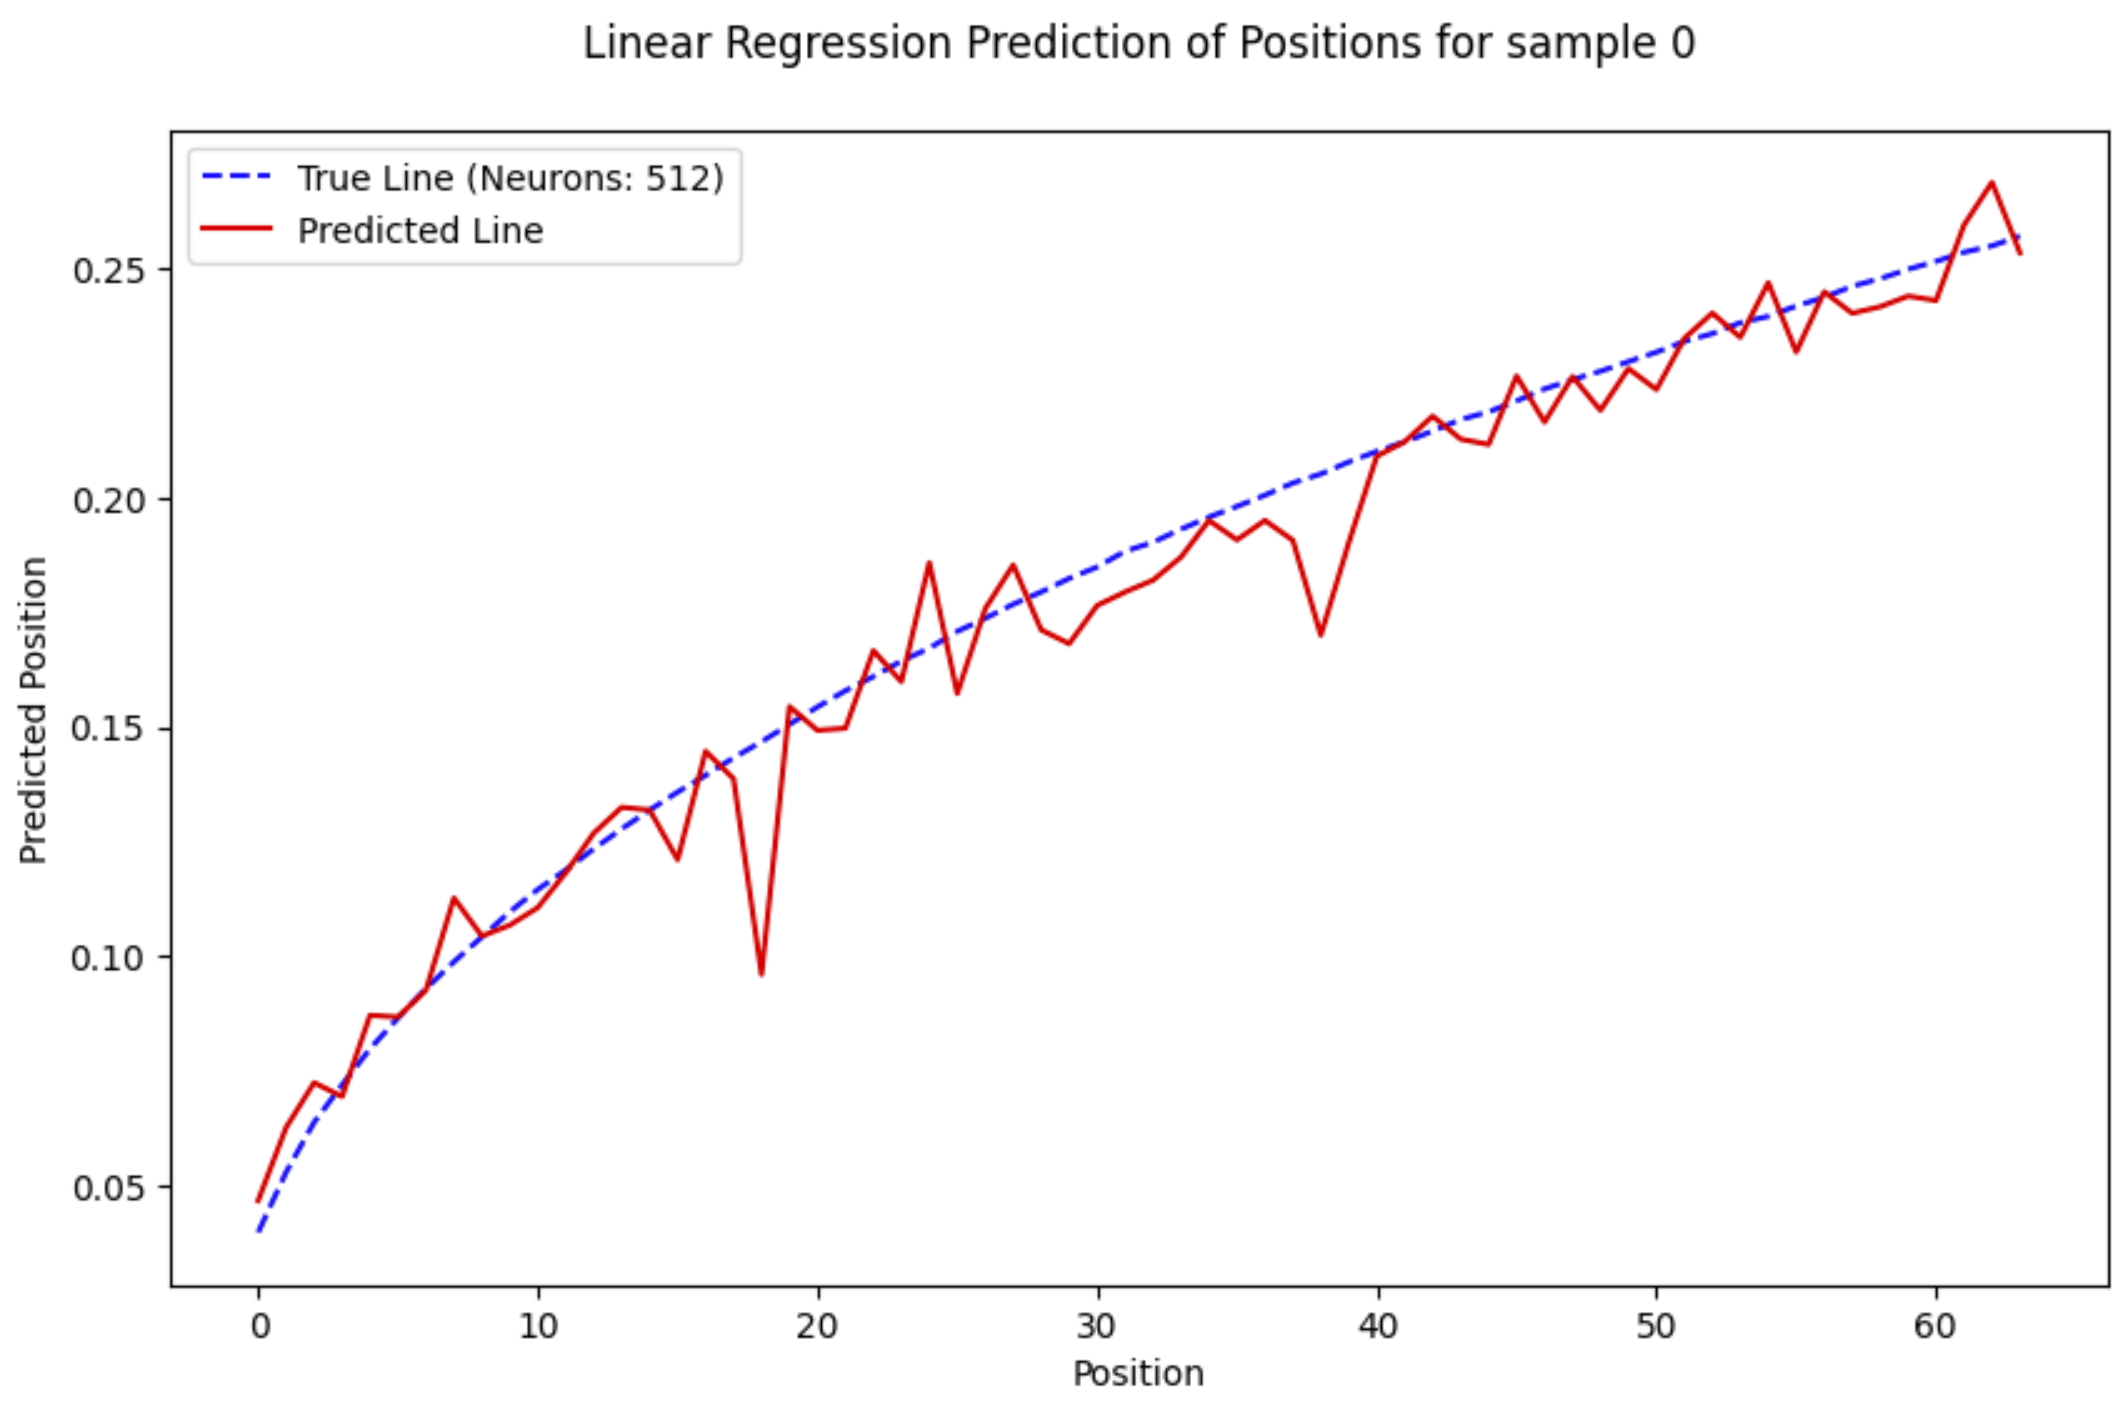
\includegraphics[width=\columnwidth]{single_sample_pred_post_LN_64_ctx.png}
\caption{Position predictions from post-LN activations for a single sample. The model accurately predicts positions 0-63 despite the absence of explicit positional embeddings.}
\label{fig:single-sample-pred}
\end{figure}

\subsubsection{Circuit Analysis: Information Flow}

We trace how positional information flows through the network by analyzing activations at each component. A key insight is that positional information undergoes a \textbf{representation transformation}: initially there is no signal at the input, then position becomes encoded primarily in the \textit{directional structure} of activations after attention (with variance as a secondary signal), and finally LayerNorm \textit{linearizes} this complex encoding into a simple norm-based signal that is trivially decodable by a linear probe.

\paragraph{Attention Patterns.}
The attention pattern depends critically on the initialization scale $\sigma$ of embedding vectors. We identify three distinct regimes. When $\sigma$ is small ($\sigma \ll 1/\sqrt{d}$), attention scores $QK^\top$ are negligible, yielding near-uniform attention weights $A_{ij} \approx 1/i$ for all $j \leq i$. For medium $\sigma$ corresponding to Xavier initialization ($\sigma \approx 1/\sqrt{d}$), the diagonal dominates while off-diagonal elements remain approximately uniform within the causal mask. When $\sigma$ is large ($\sigma \gg 1/\sqrt{d}$), attention concentrates on random positions due to large score variance, breaking the position-encoding mechanism. The optimal regime for position encoding is the uniform or medium-$\sigma$ case, where attention weights create position-dependent variance in outputs. Figure~\ref{fig:attention-patterns} visualizes these three regimes.

\begin{figure}[htbp]
\centering
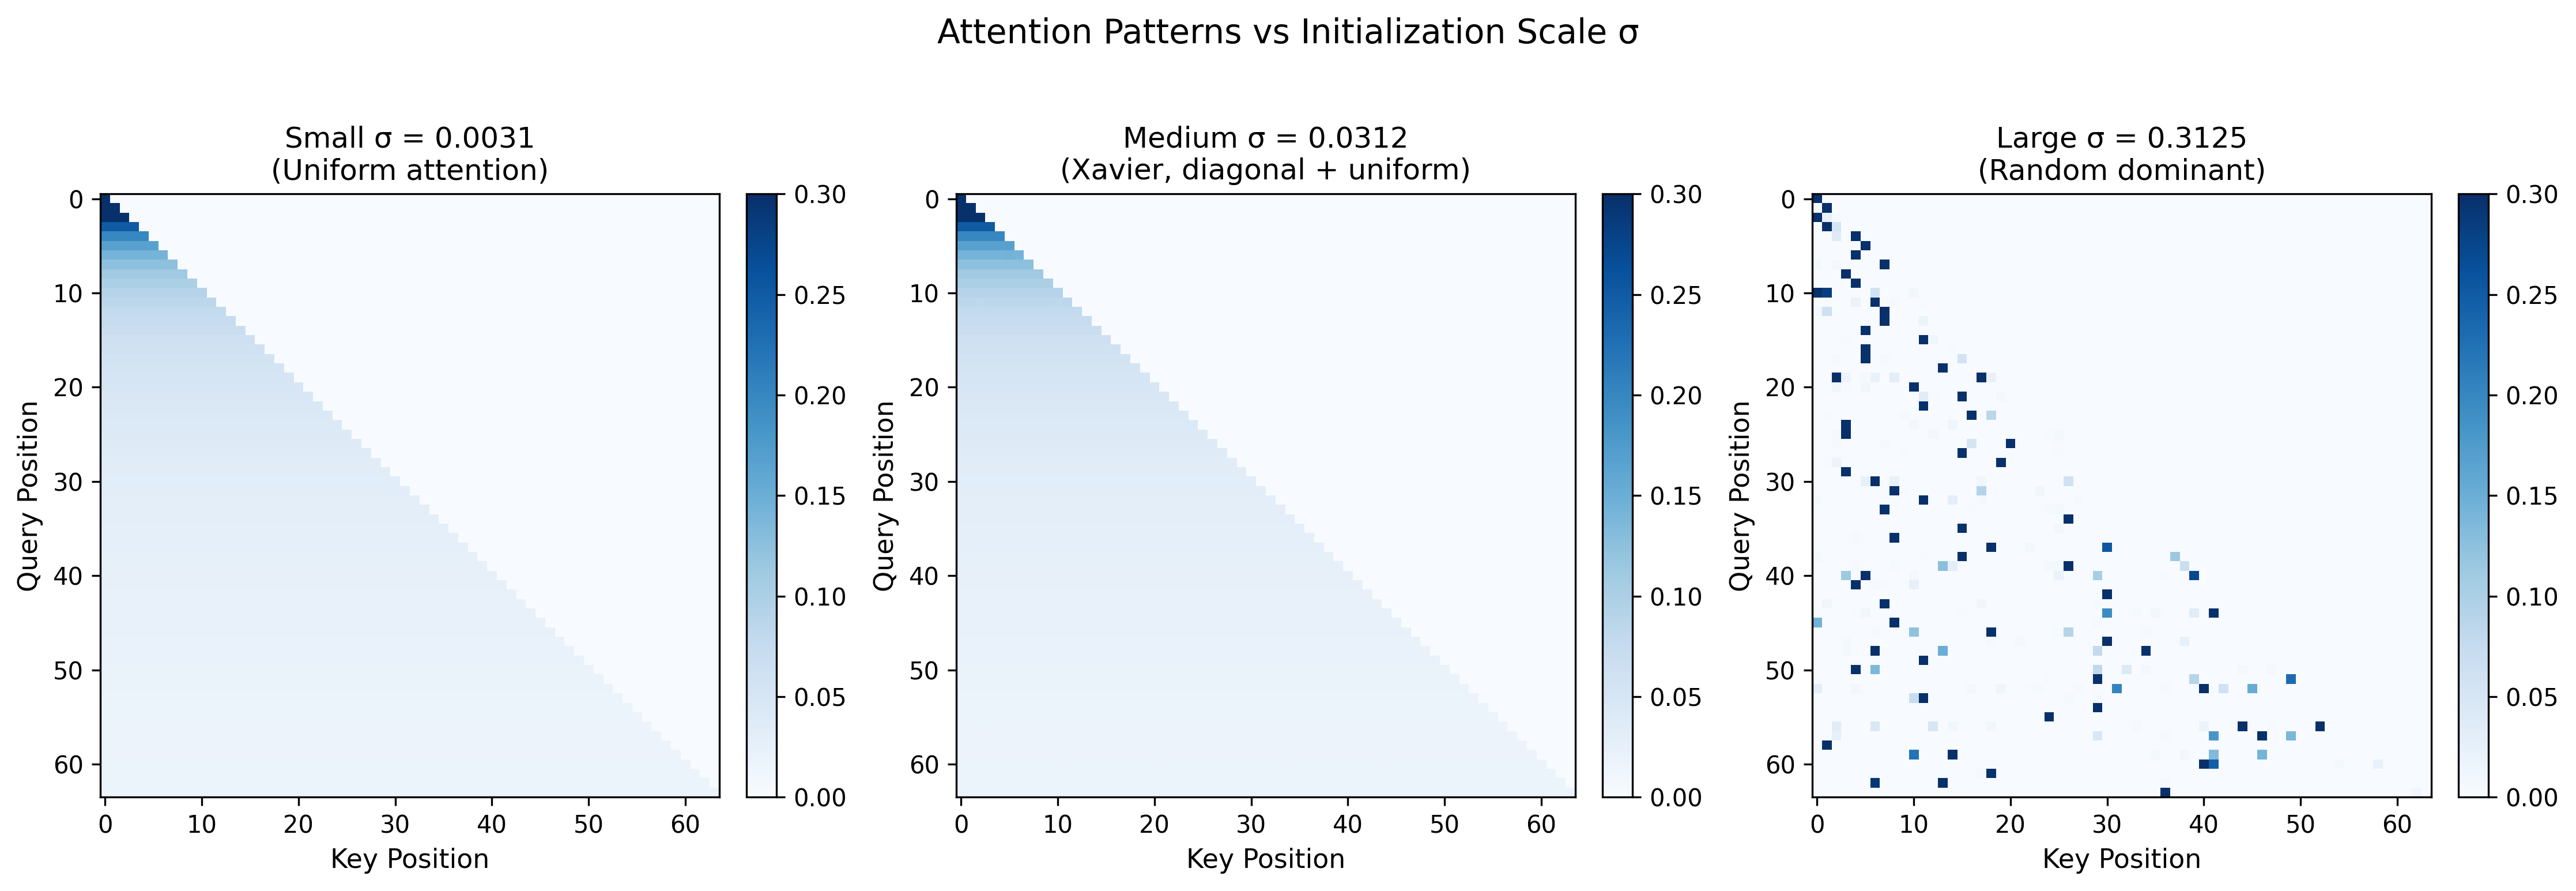
\includegraphics[width=\columnwidth]{attention_std_phases.png}
\caption{Attention patterns (after softmax) for three initialization scales. Left: small $\sigma$ yields near-uniform attention. Center: Xavier initialization produces diagonal-dominant pattern with uniform lower triangle. Right: large $\sigma$ causes random positions to dominate.}
\label{fig:attention-patterns}
\end{figure}

\paragraph{Post-Attention Variance Signal.}
After attention, the mean activation across channels remains position-independent, but the variance exhibits clear monotonic decay with position following $\text{Var}(z_i) \propto 1/(i+1)$. This variance signal arises because each position $i$ aggregates context from $i$ previous tokens, creating position-dependent spread in the weighted sum. Figure~\ref{fig:variance-decay} demonstrates this monotonic decay.

\begin{figure}[htbp]
\centering
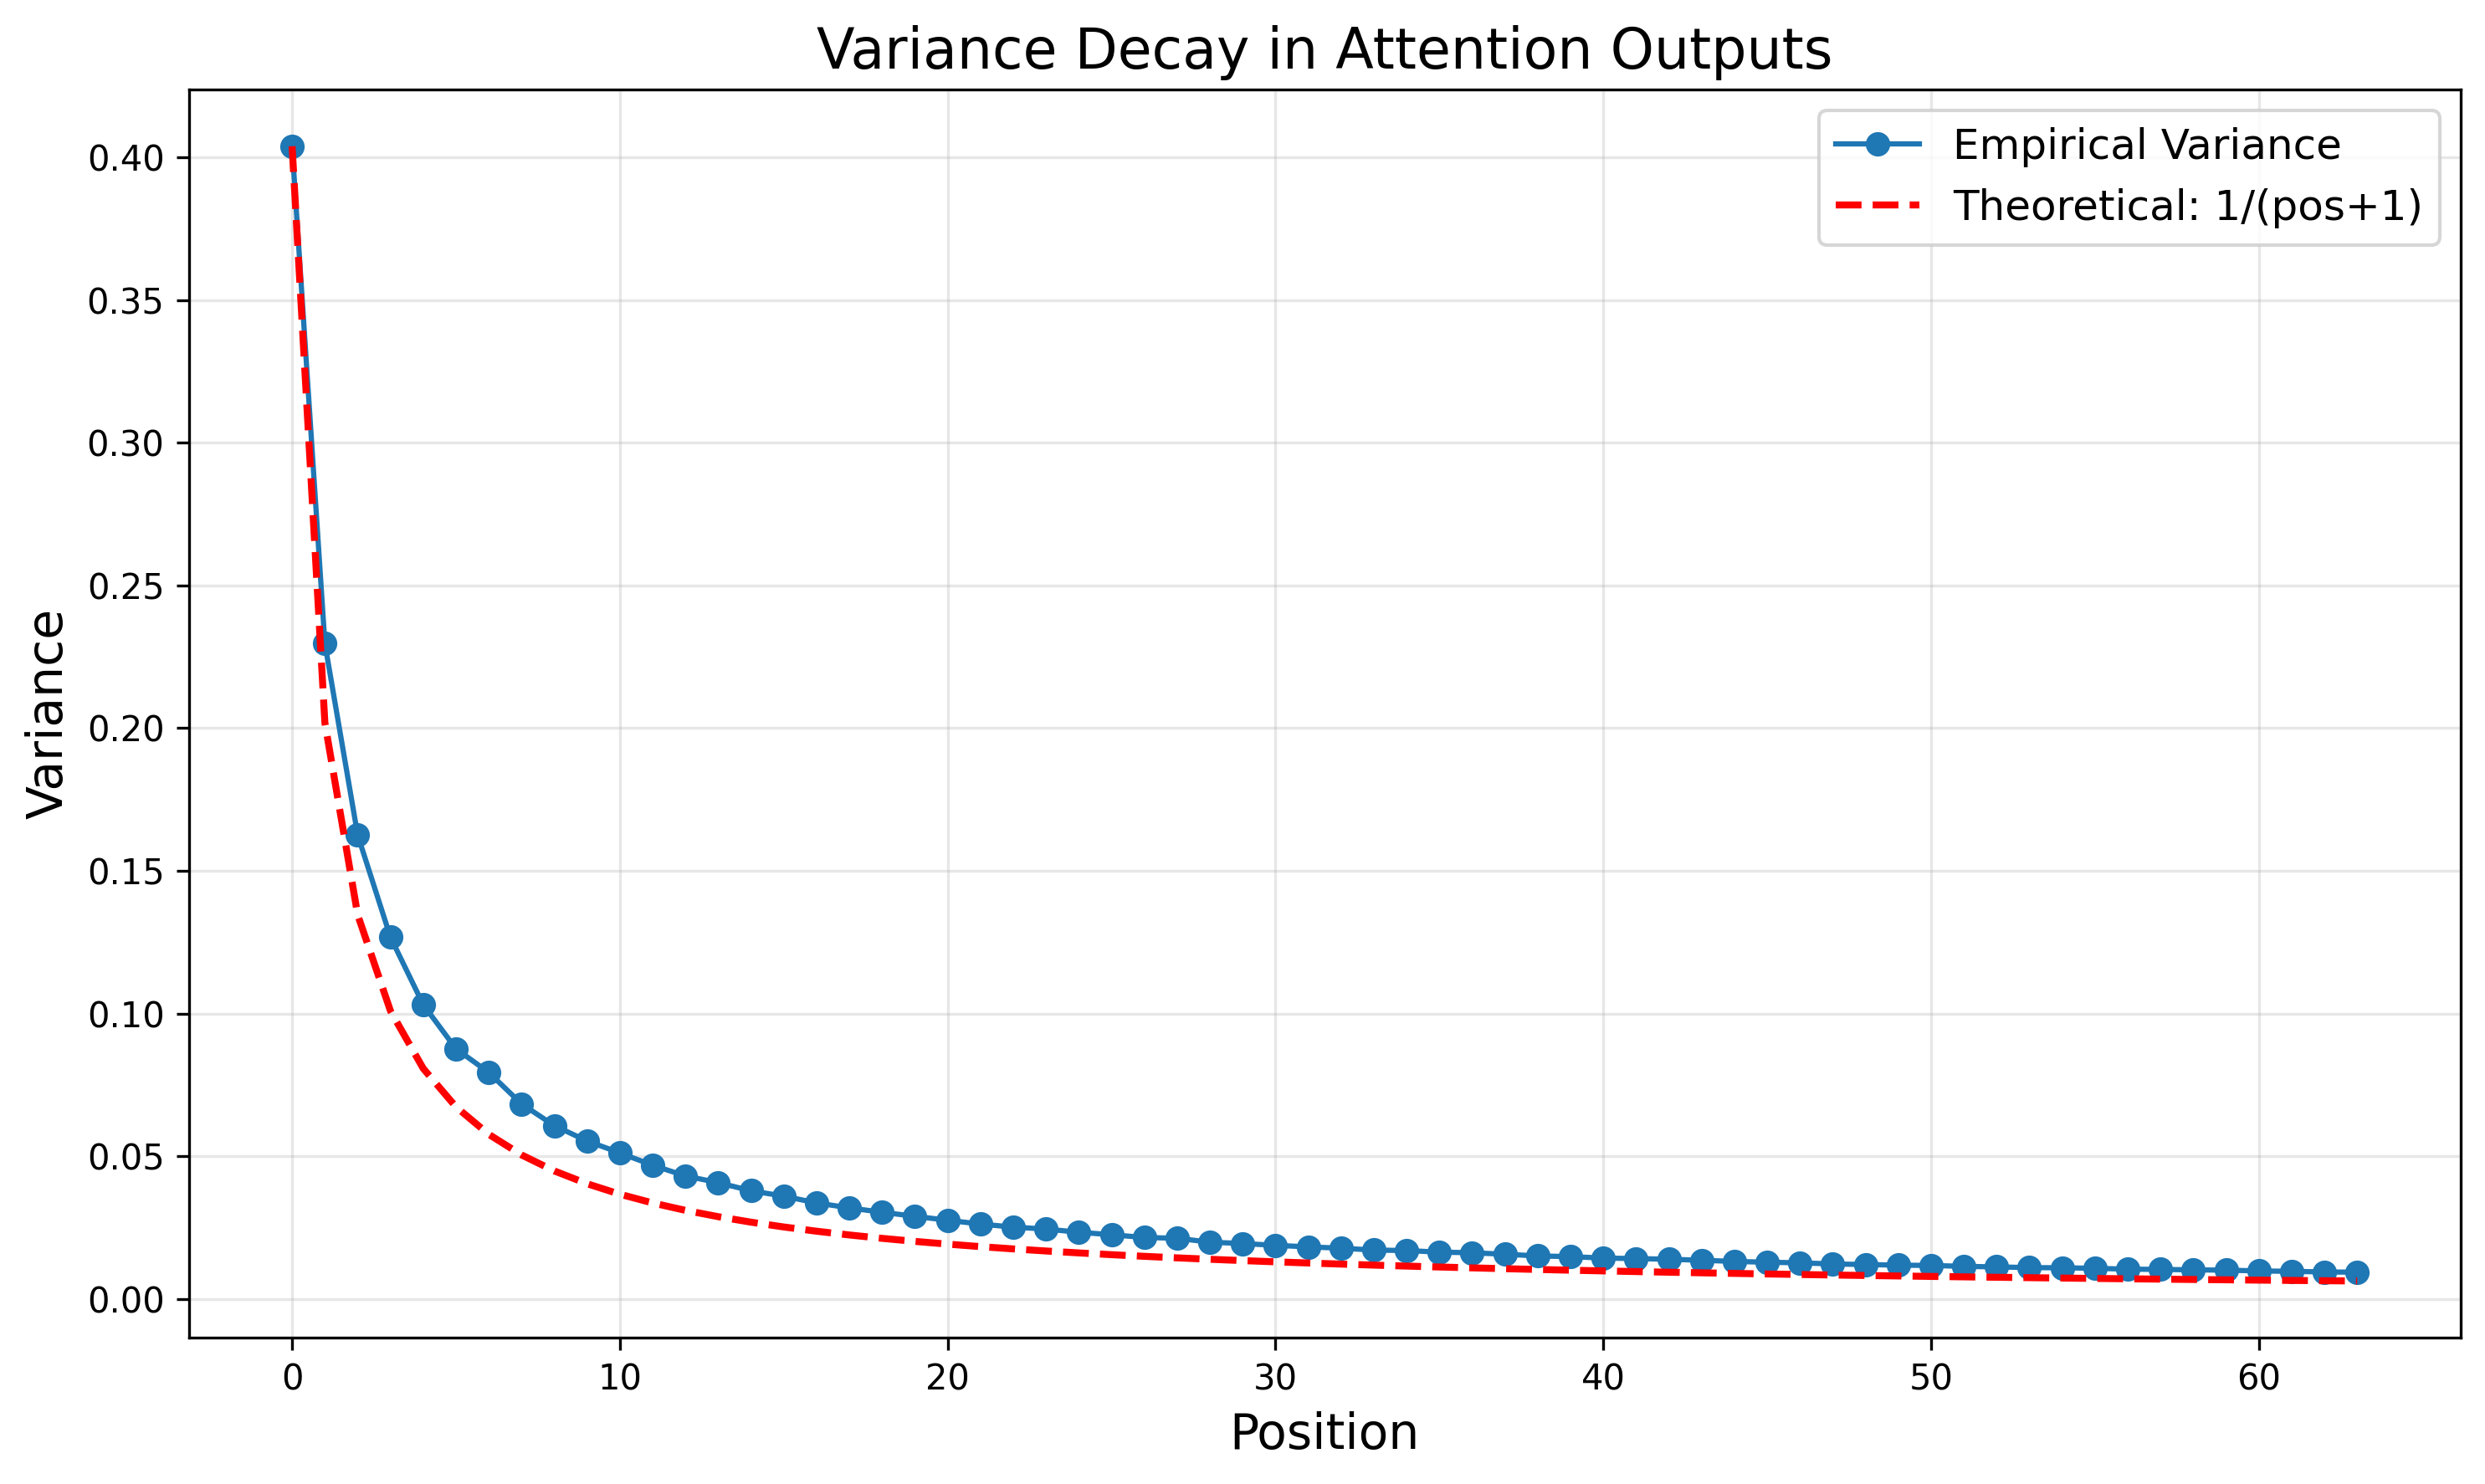
\includegraphics[width=\columnwidth]{variance_decay.png}
\caption{Post-attention variance decay as a function of position. The variance decreases monotonically, providing a clear positional signal that LayerNorm can read.}
\label{fig:variance-decay}
\end{figure}

\paragraph{Post-LN Activations.}
LayerNorm computes the standard deviation $\sigma_i$ across channels at each position, effectively reading out the variance signal. Since $\sigma_i$ varies monotonically with position, the normalization process encodes position-dependent input variance into the output norm. Critically, LayerNorm does not simply preserve positional information---it \textit{linearizes} it. Before LayerNorm, position is encoded in complex, high-dimensional directional structure that yields poor linear decodability ($R^2=0.04$). After LayerNorm, the same information becomes a near-linear function of output norm ($R^2_{\text{norm}}=0.88$), making position trivially decodable by a linear probe. Additionally, at the population level, averaging across many samples reveals smooth monotonic patterns due to position-correlated token distributions.

\begin{figure}[htbp]
\centering
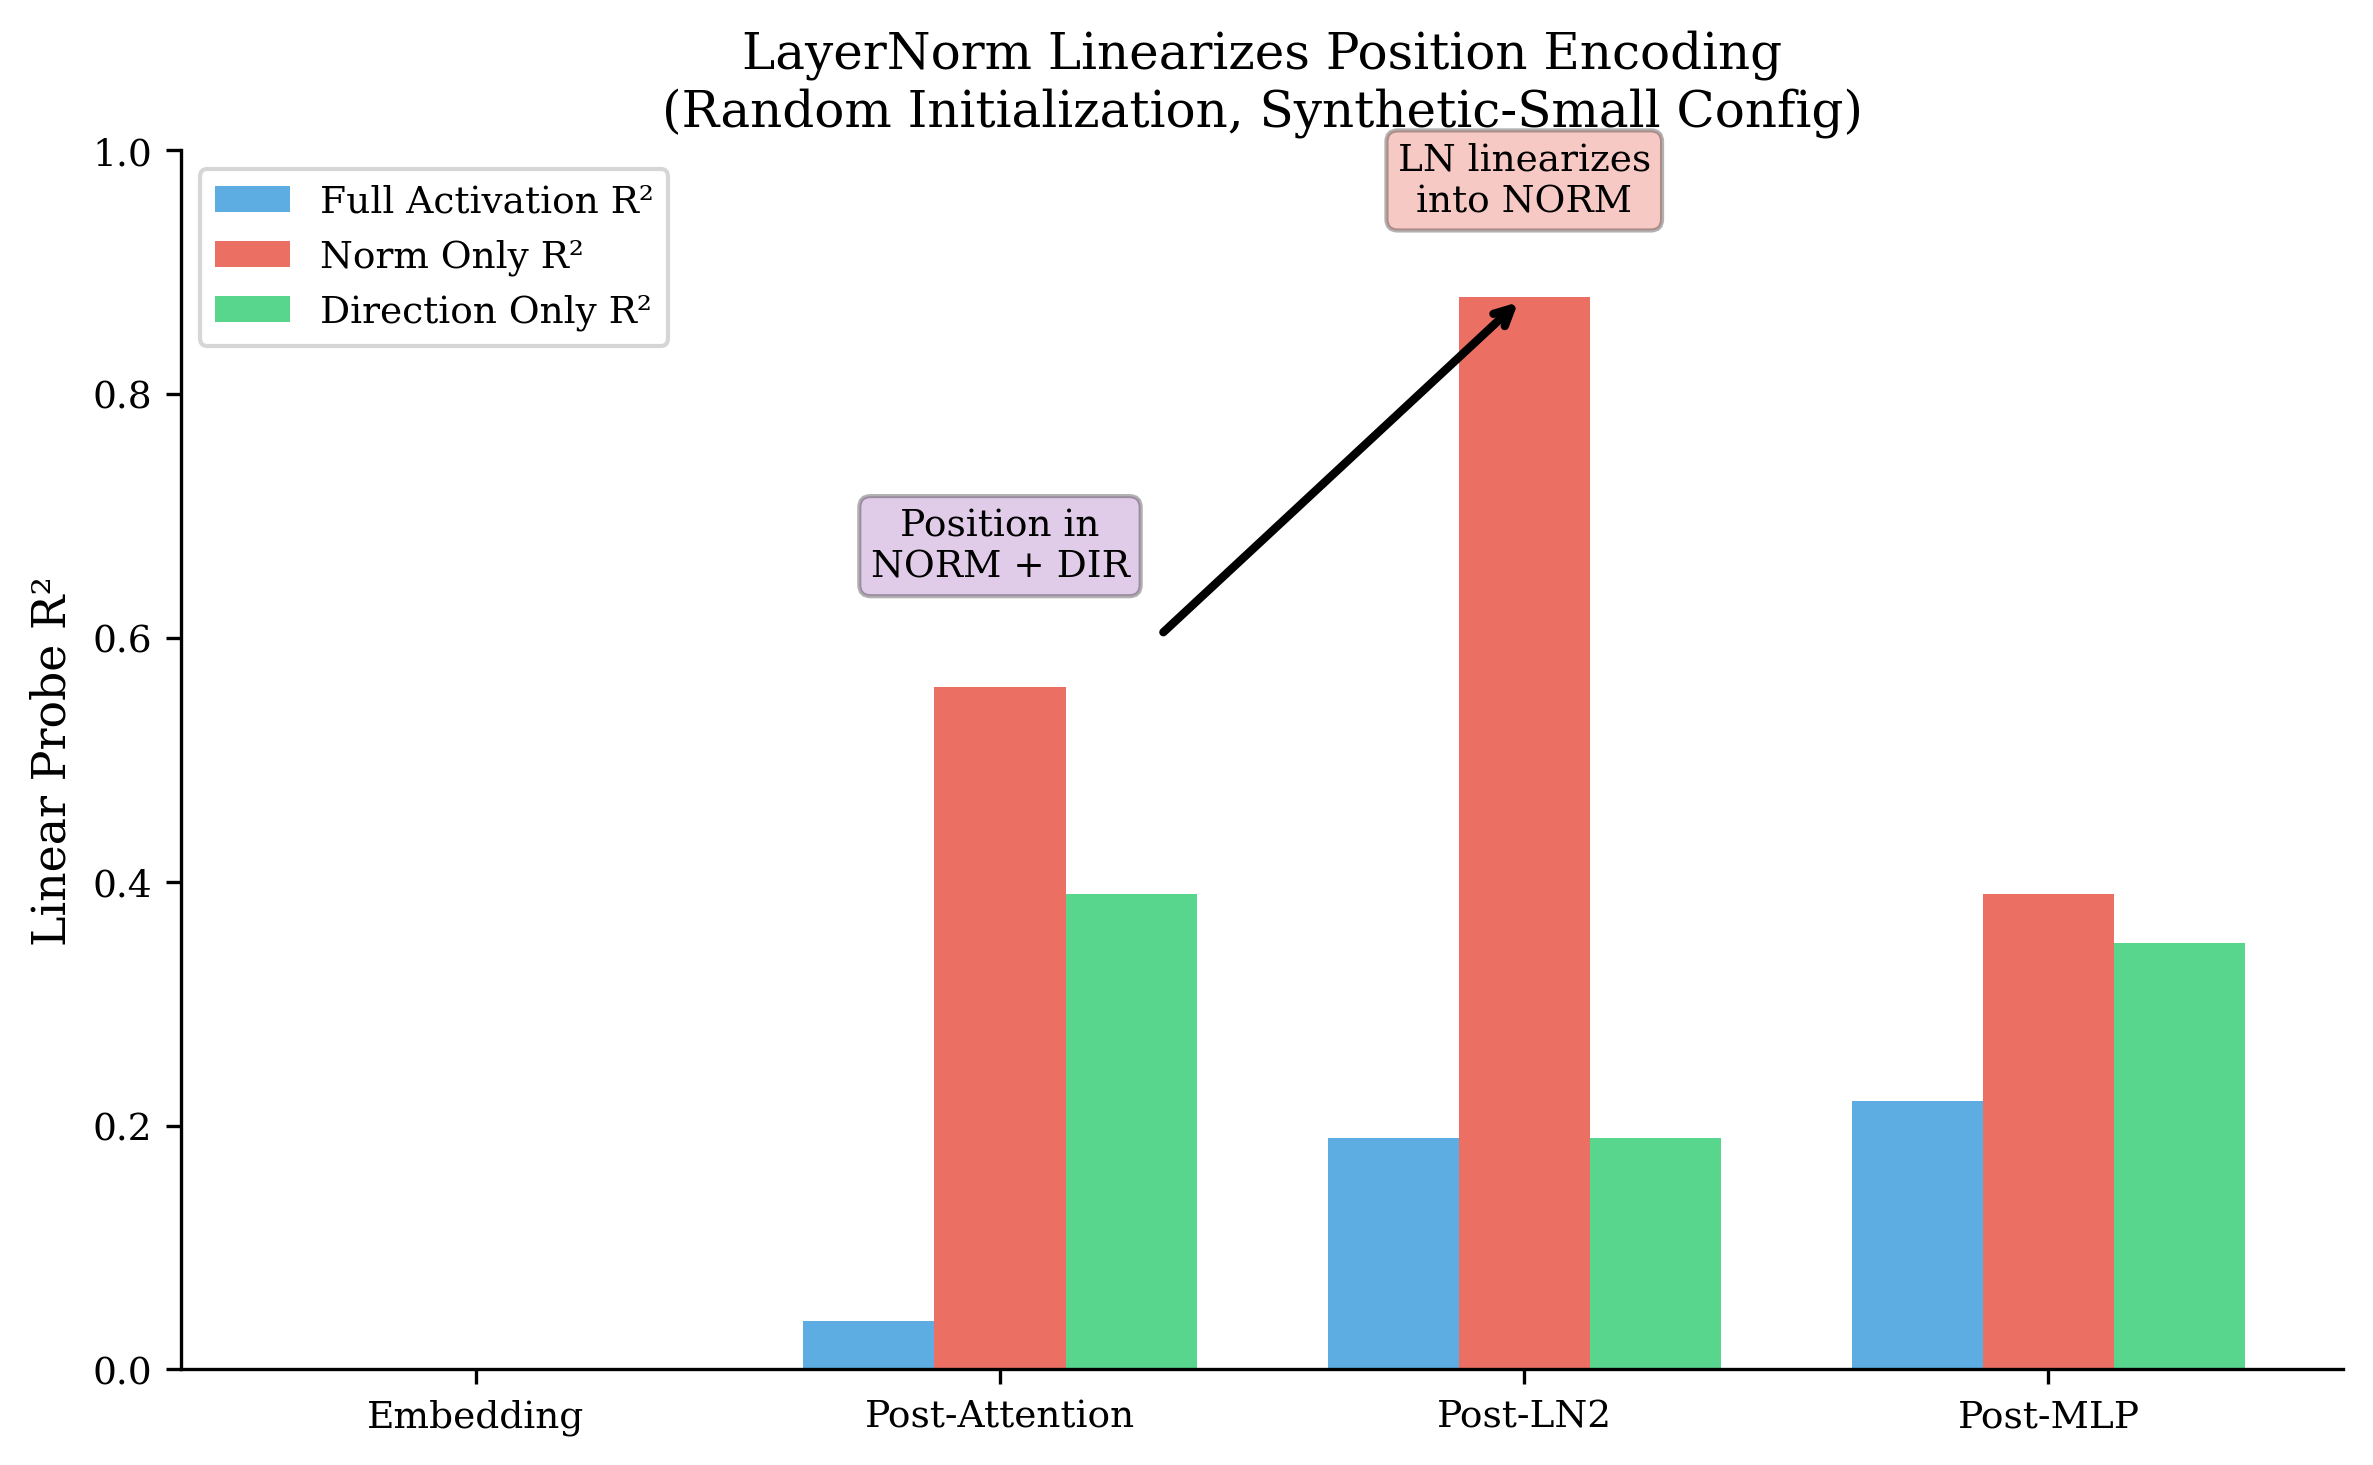
\includegraphics[width=\columnwidth]{layernorm_linearization.png}
\caption{LayerNorm linearization effect. \textbf{Left}: Before LN (post-attention), position is encoded in directional structure ($R^2_{\text{dir}}=0.39$) and norm ($R^2_{\text{norm}}=0.56$), but full activations yield poor linear decodability ($R^2_{\text{full}}=0.04$). \textbf{Right}: After LN, norm dominates ($R^2_{\text{norm}}=0.88$) while direction R\textsuperscript{2} drops to $0.19$. LN transforms complex directional encoding into simple norm-based signal.}
\label{fig:ln-linearization}
\end{figure}

Figure~\ref{fig:ln-linearization} illustrates this linearization effect. The key insight is that LayerNorm's normalization step converts the nonlinear relationship between position and activation structure into a near-linear relationship. Figure~\ref{fig:layernorm-paradox} visualizes the population-level patterns across 30K samples.

\begin{figure*}[htbp]
\centering
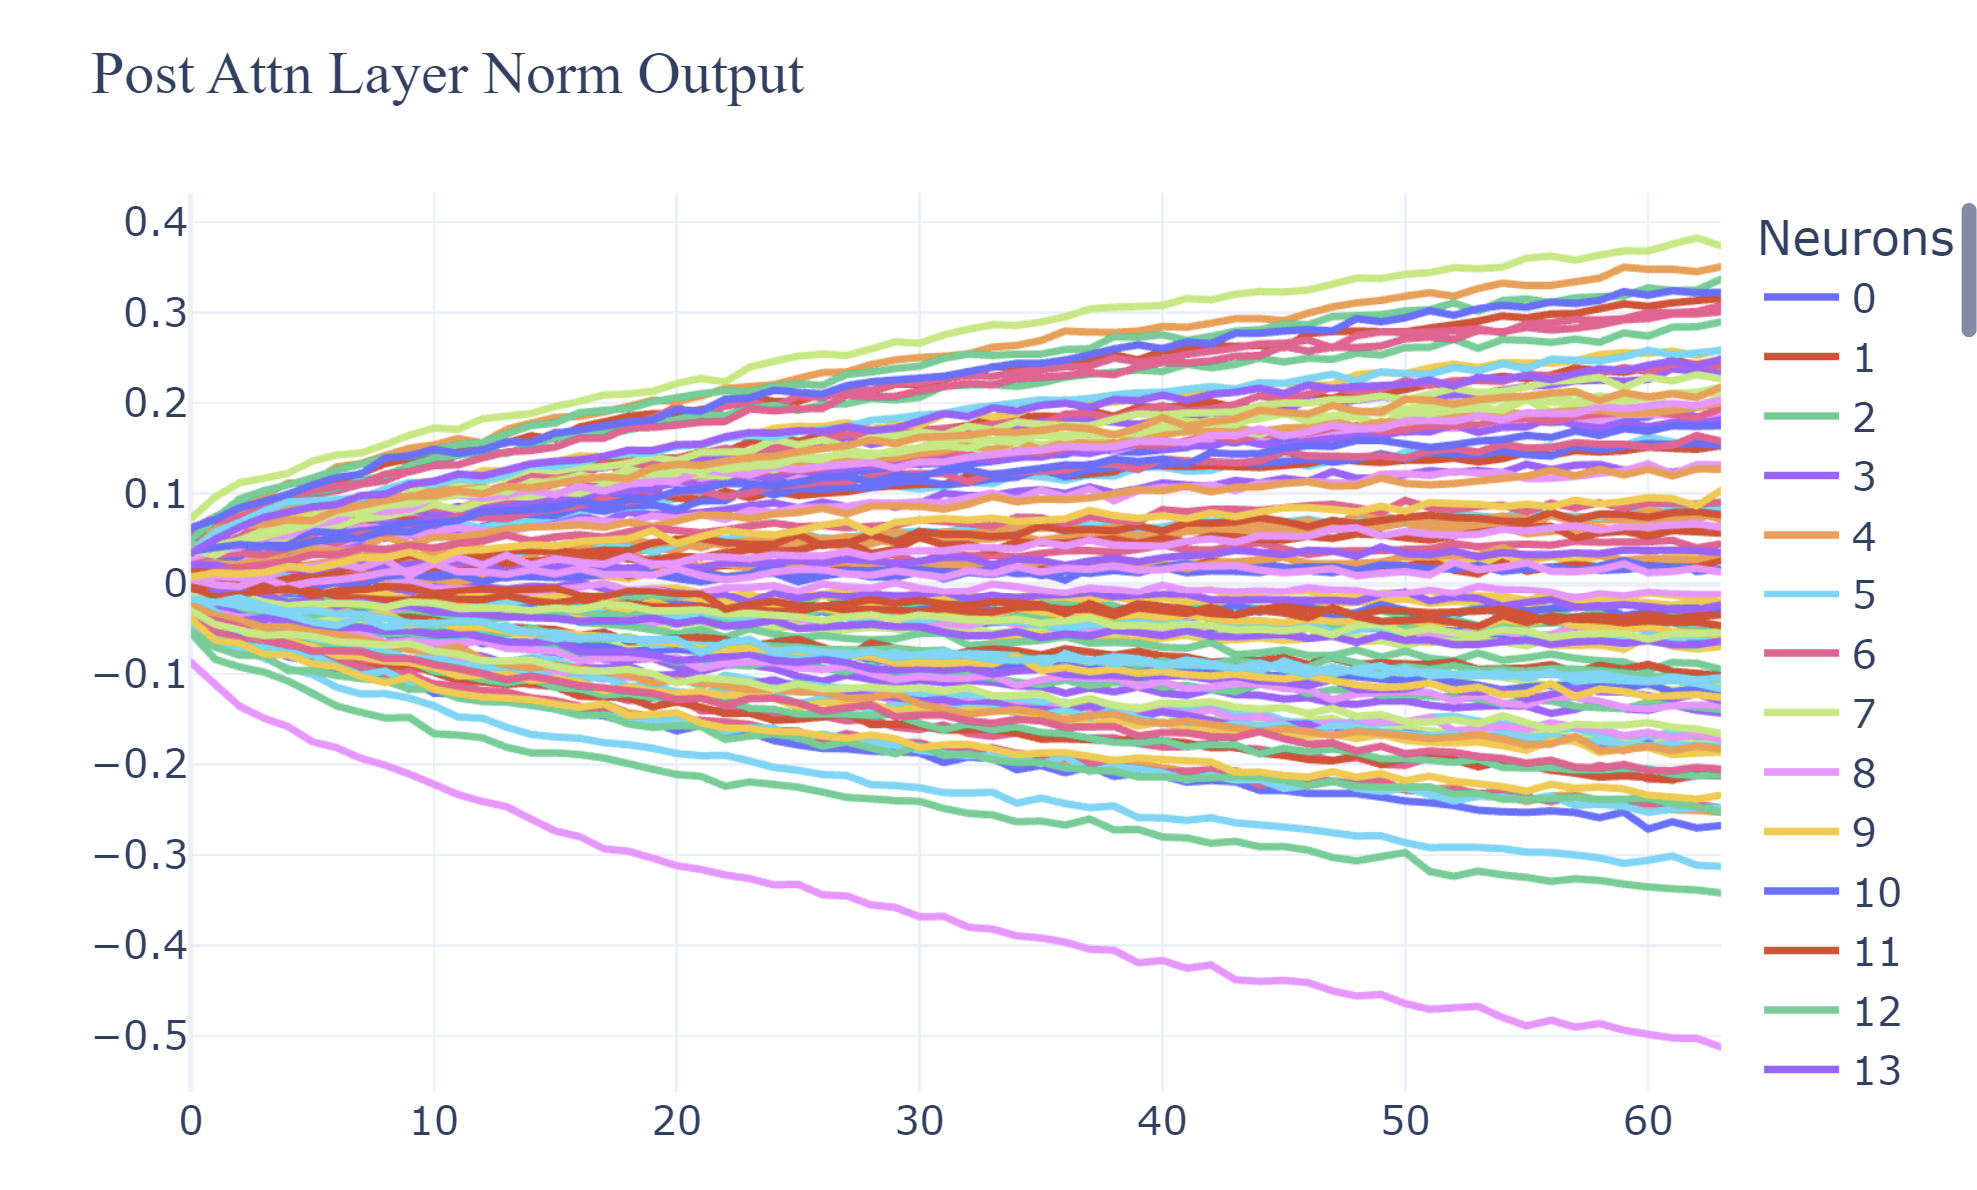
\includegraphics[width=\textwidth]{post_attn_ln_output_30K_samples_64_ctx.png}
\caption{Post-LN activation patterns across 30K samples and 64 positions. Despite LayerNorm normalizing each position individually, clear positional structure emerges in the population-level activations. The heatmap reveals distinct patterns at different positions, demonstrating how positional information is preserved through population statistics.}
\label{fig:layernorm-paradox}
\end{figure*}

\subsubsection{MLP Position Decoding}\label{sec:mlp-decoding}

The MLP extracts position information by exploiting the approximate orthogonality of token embeddings in high-dimensional spaces. We derive a constructive proof showing how this decoding works.

With near-uniform attention weights $A_{ij} \approx 1/i$, the attention output at position $i$ is $z_i \approx \frac{1}{i} \sum_{j=1}^{i} v_j$ where $v_j = W_V x_j$ are the value vectors. A key property of random Gaussian initialization in high dimensions ($d \gg 1$) is that it produces nearly orthogonal vectors: $v_k \cdot v_j \approx 0$ when $k \neq j$, while $v_k \cdot v_k = \|v_k\|^2 > 0$. We exploit this orthogonality for constructing a decoding vector.

Since the input to attention is normalized with LayerNorm, the value vectors are $v_j = W_V \cdot \text{LN}(E_j)$ where $E_j$ is the embedding for token $j$. We construct a single decoding vector $w$ as the sum of all normalized embeddings transformed by $W_V$:
\begin{equation}
w = W_V \cdot \sum_{j=1}^{N} \text{LN}(E_j)
\end{equation}

For each token $j$, we compute the dot product $w \cdot v_j$. Due to orthogonality, each token contributes approximately the same positive value $c \approx \|v\|^2$. At position $i$, summing the contributions from the first $i$ tokens gives:
\begin{equation}
\text{decoded}(i) = \sum_{j=1}^{i} (w \cdot v_j) \approx i \cdot c
\end{equation}

Normalizing by the mean contribution $\bar{c}$ recovers the position. We validate this empirically using embeddings with $d=1024$ and vocabulary size 5000, achieving \textbf{Pearson correlation $r = 0.999$} between decoded and true positions. Figure~\ref{fig:mlp-contributions} shows individual contributions $w \cdot v_j$ at several positions, where green bars indicate tokens contributing to position $i$. Figure~\ref{fig:mlp-decoding} shows the cumulative sum growing linearly with position.

\begin{figure}[htbp]
\centering
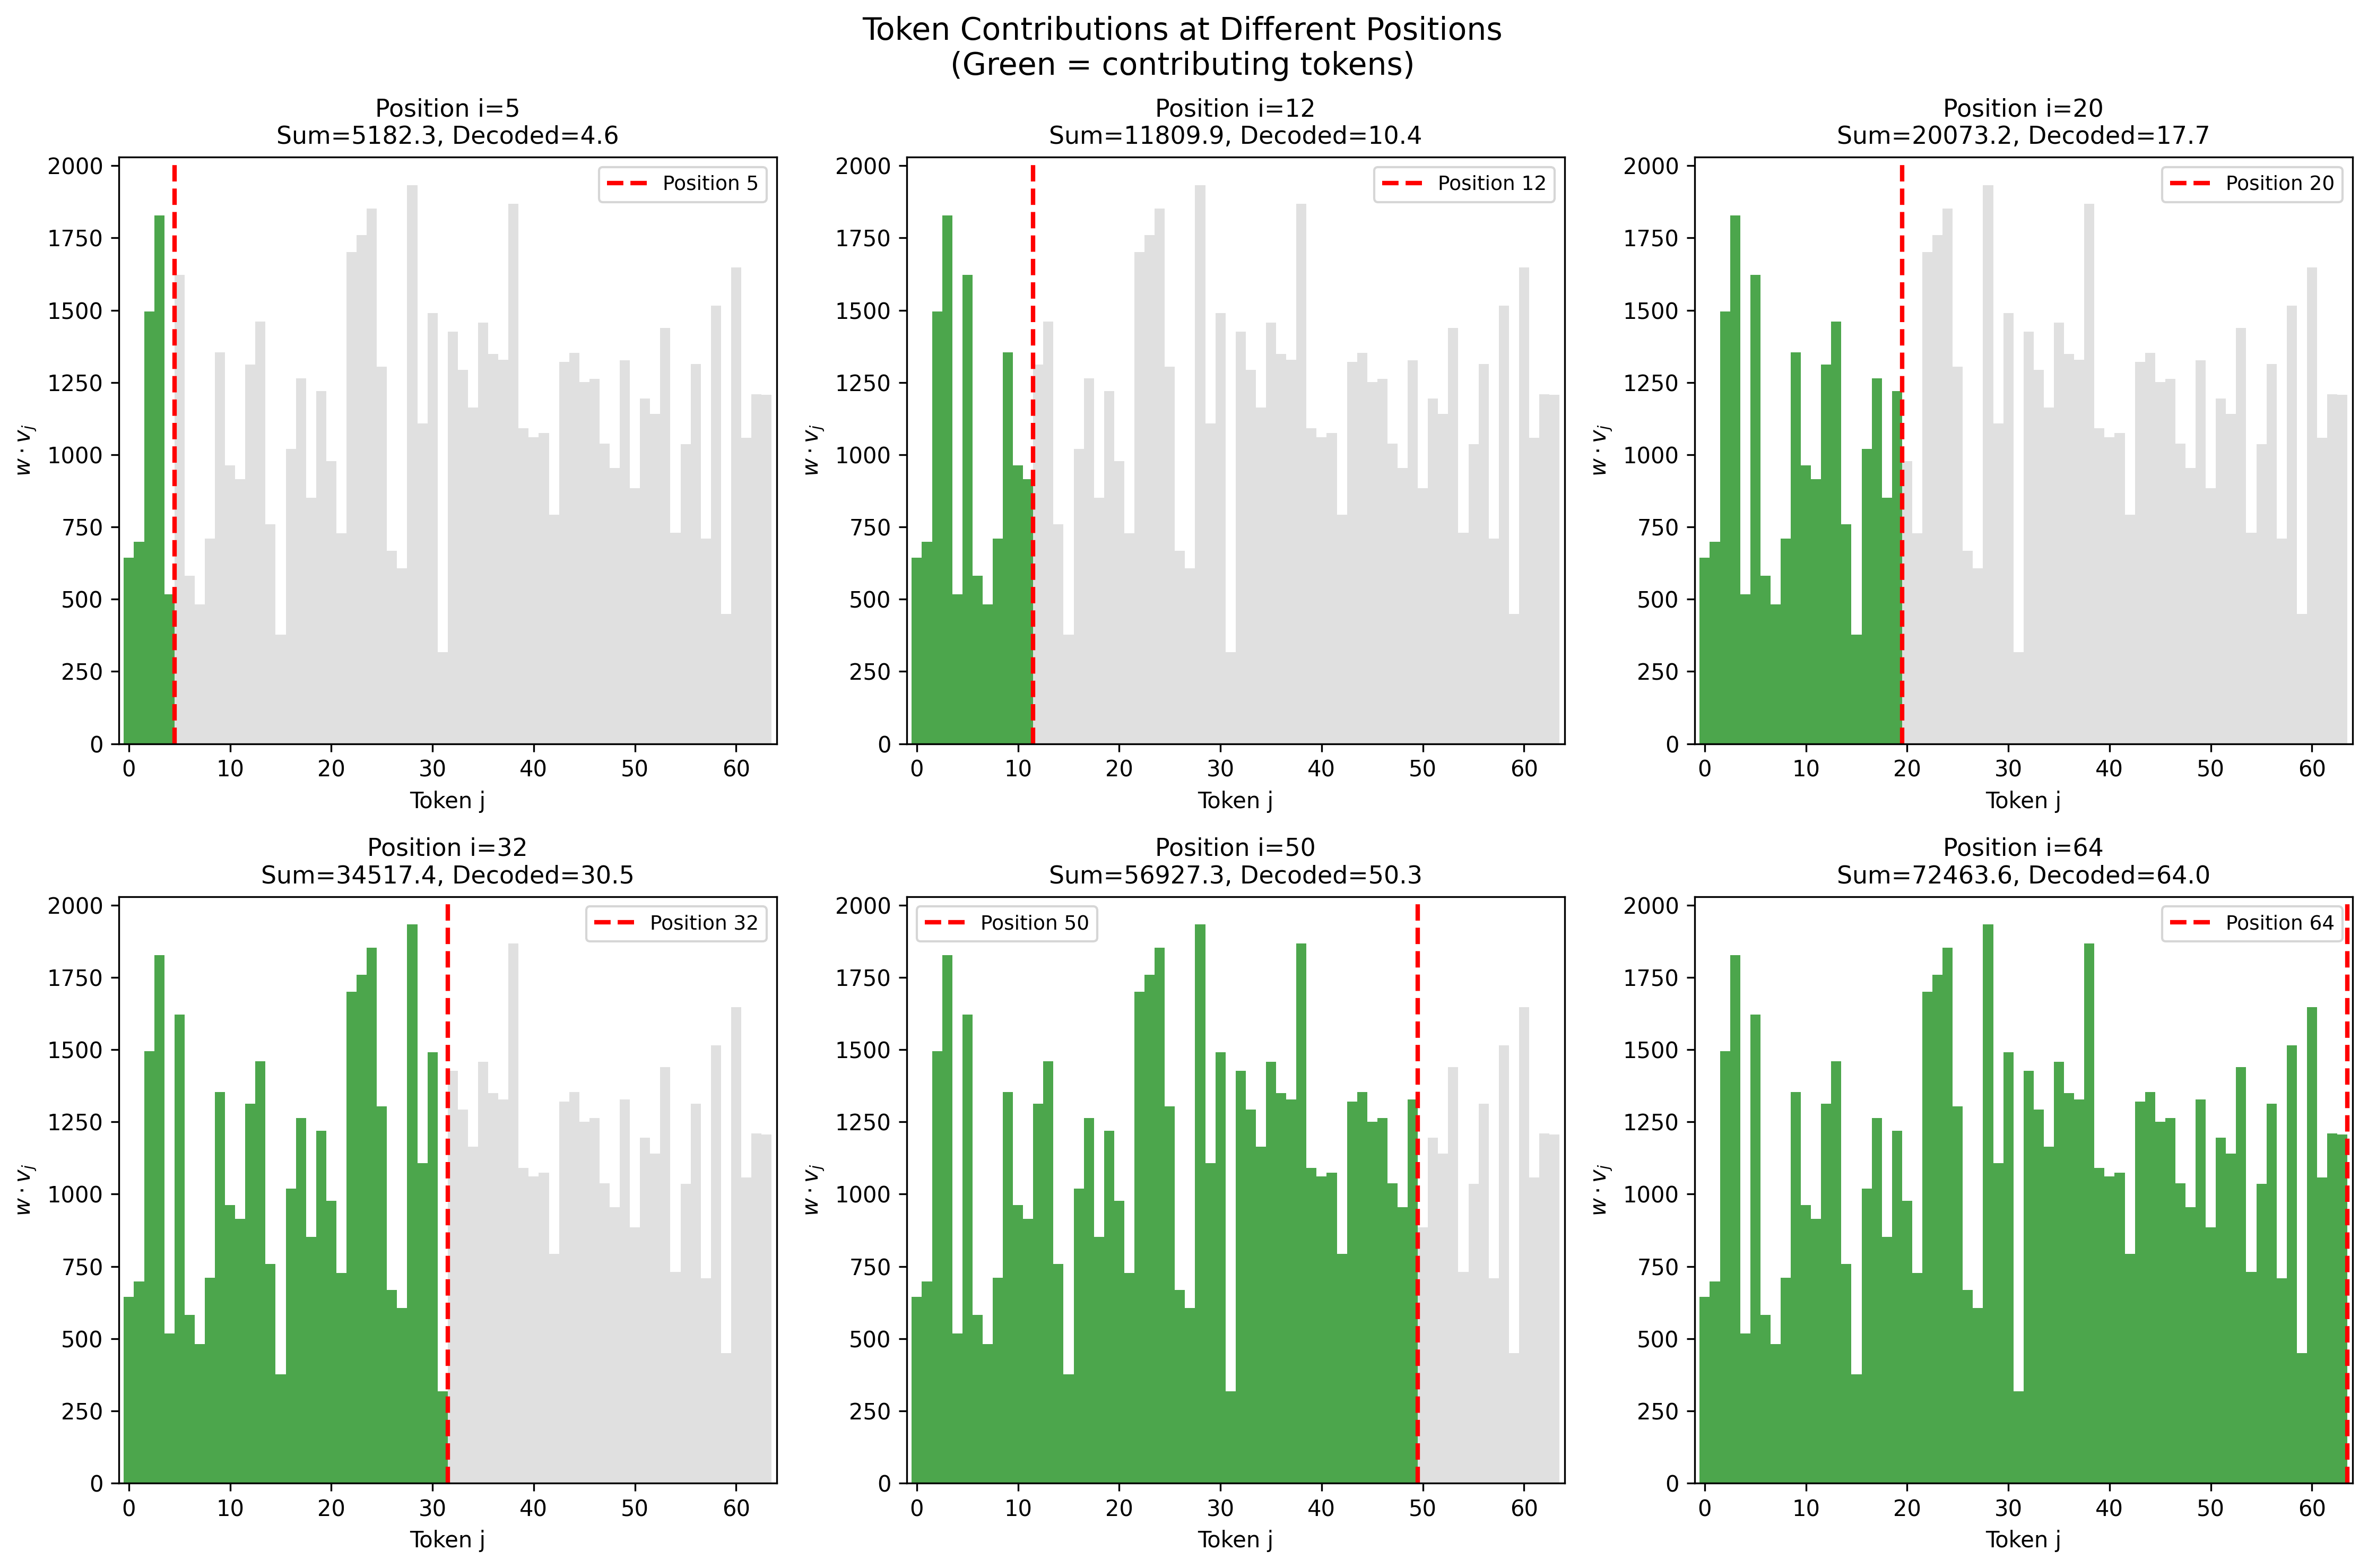
\includegraphics[width=\columnwidth]{mlp_decoding_contributions.png}
\caption{MLP position decoding via the decoding vector $w$. Each bar shows $w \cdot v_j$ for token $j$. At position $i$, the green bars (indices $j \leq i$) are tokens included in the attention output. The decoded value is the sum of green bars, which grows linearly with $i$.}
\label{fig:mlp-contributions}
\end{figure}

\begin{figure}[htbp]
\centering
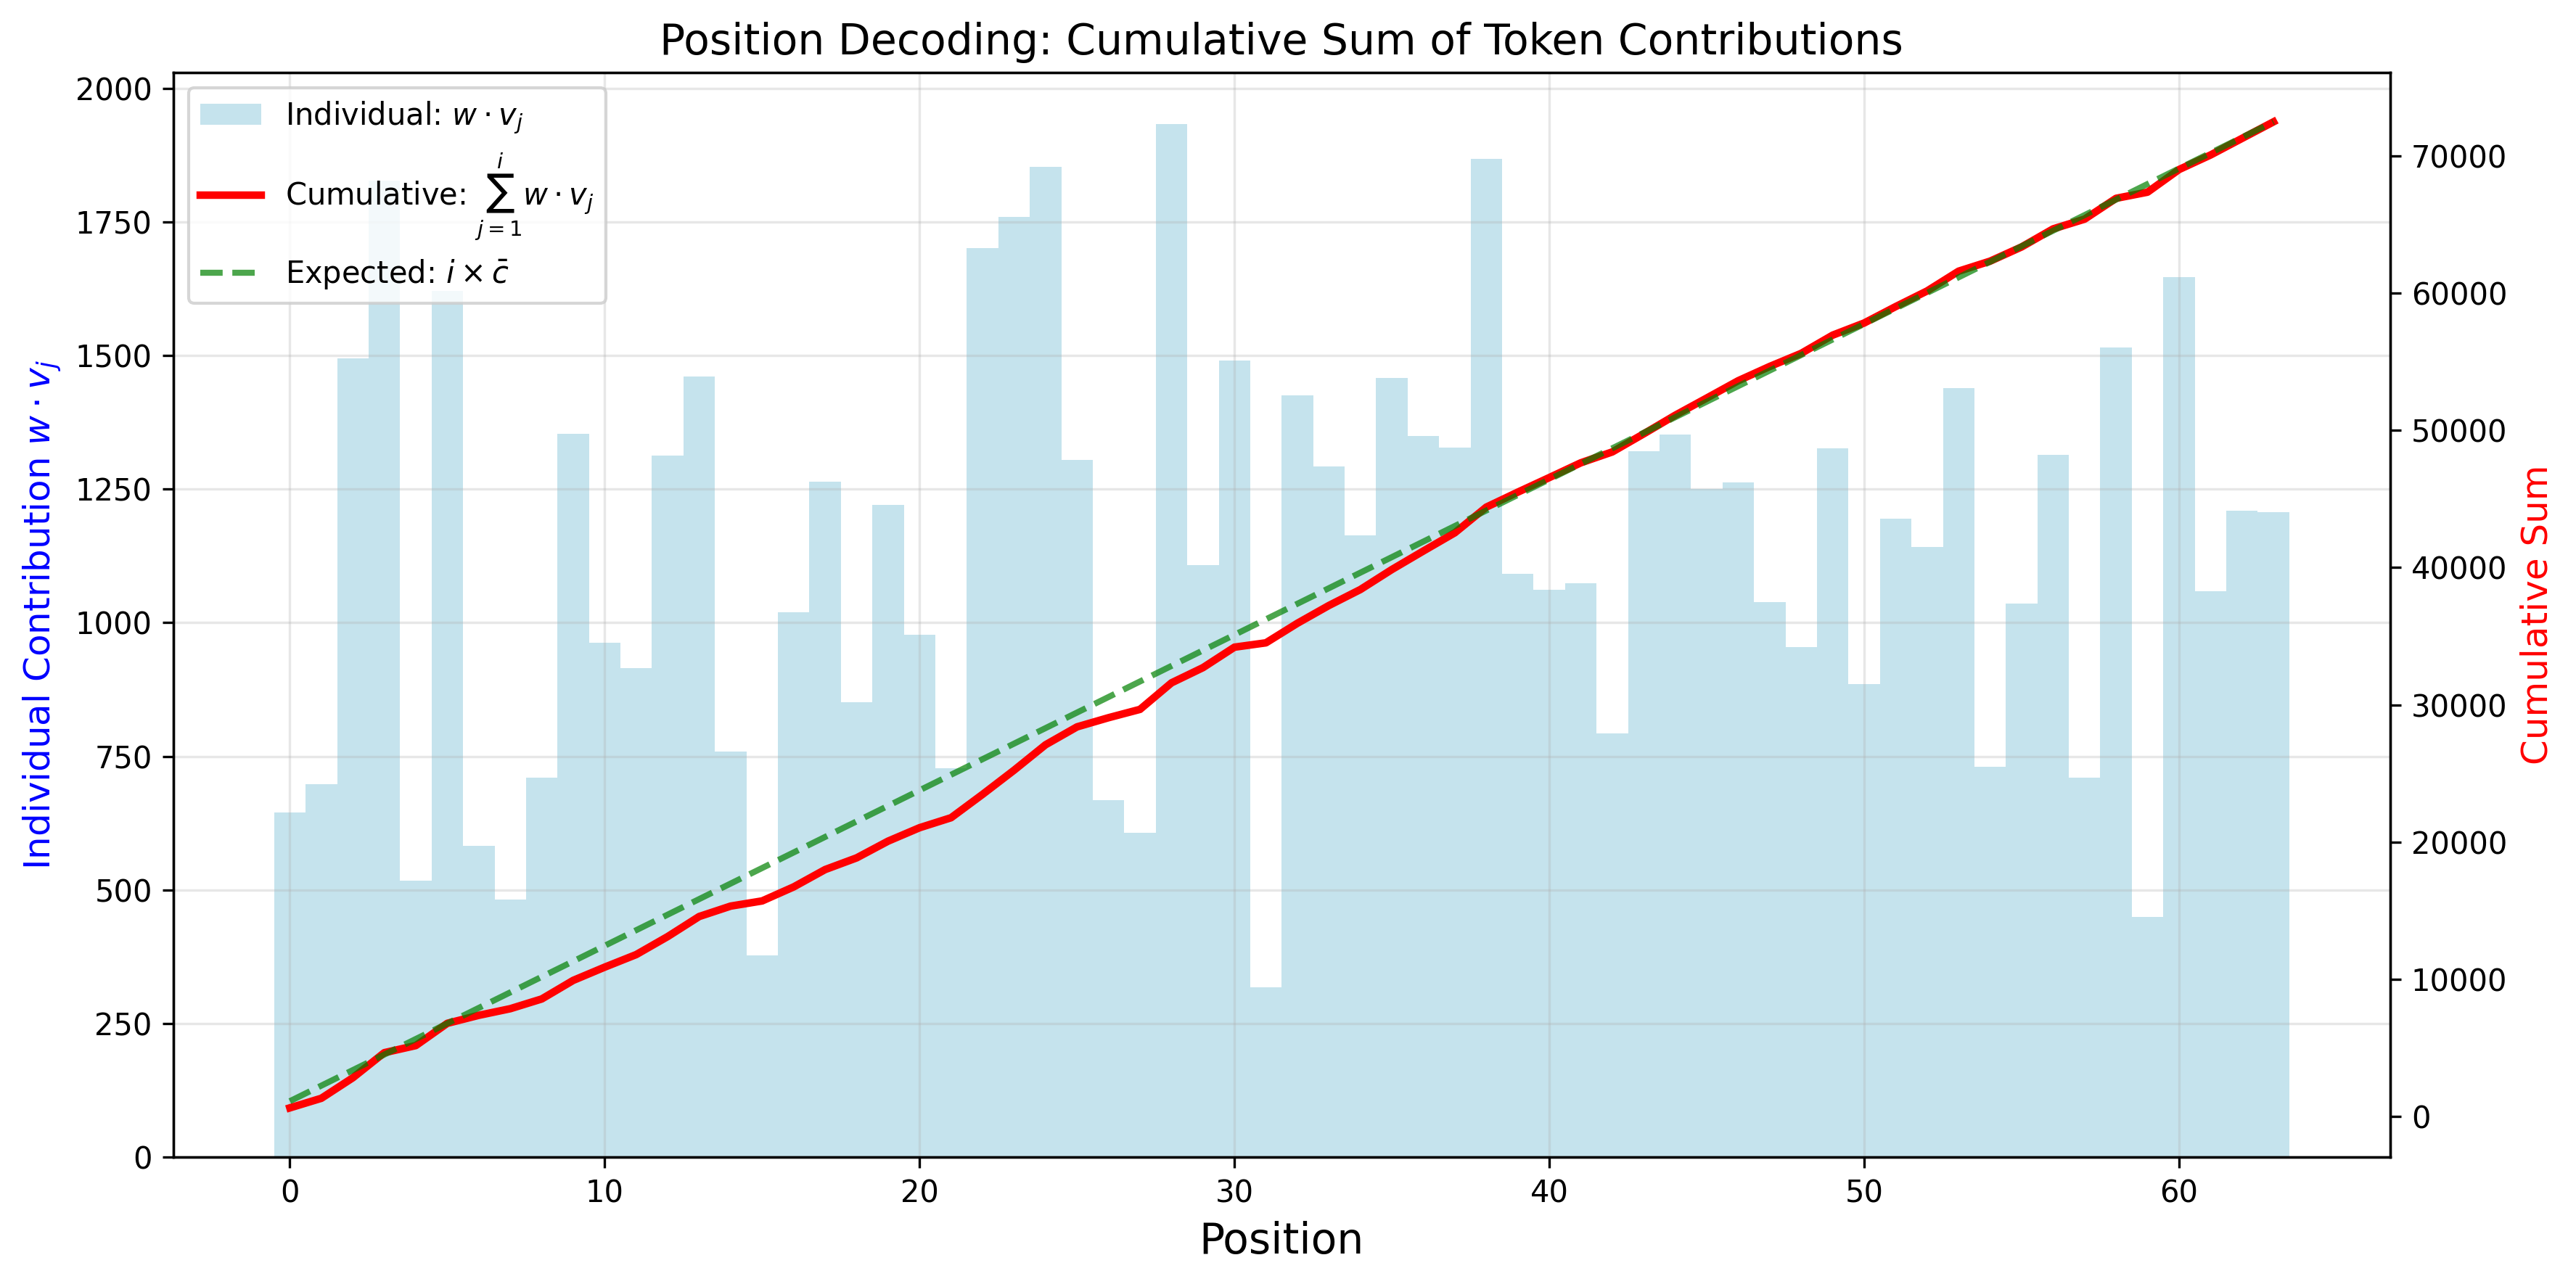
\includegraphics[width=\columnwidth]{mlp_decoding_summary.png}
\caption{Position decoding overview. Blue bars show individual contributions $w \cdot v_j$ which are approximately constant. The red line shows the cumulative sum $\sum_{j=1}^{i}(w \cdot v_j)$ which grows linearly with position. Dividing by the mean contribution recovers the position.}
\label{fig:mlp-decoding}
\end{figure}

\subsection{Natural Language Dataset}

We evaluate on natural language using the WikiText-2 dataset, where token repetition patterns play a crucial role. Unlike synthetic data, natural language exhibits position-correlated token distributions—punctuation tends to appear at sentence ends, articles at beginnings, and different parts of speech show clear position preferences. The model maintains \textbf{over 95\% accuracy} on position prediction, demonstrating that the mechanism generalizes to real-world text.

\subsubsection{Token Diversity Threshold}

We investigate the minimum token diversity required by systematically varying the number of distinct tokens in 64-token sequences. With all identical tokens (0 distinct), the model fails completely, predicting only position 0 for all tokens. As we increase diversity to 1-8 distinct tokens, we observe gradual improvement with predictions beginning to spread across positions. The critical threshold occurs at approximately 9 distinct tokens, after which the model achieves perfect position prediction accuracy. This threshold corresponds to the minimum diversity needed to create sufficient variance in the attention score matrix.

\subsection{Vocabulary Scaling}

To understand the relationship between vocabulary size and sample requirements, we conducted experiments across vocabulary sizes from 1K to 32K tokens. We find a clear linear relationship with $R^2 > 0.99$:
\begin{equation}
\text{min\_samples} \approx 0.5 \times \text{vocab\_size}
\end{equation}
where min\_samples is the minimum number of training sequences needed to achieve over 95\% accuracy. For a realistic 32K vocabulary typical of GPT-style models, the mechanism requires 8,000-32,000 samples. These requirements are easily met in typical training scenarios. Figure~\ref{fig:vocab-scaling} visualizes this linear scaling relationship.

\begin{figure}[htbp]
\centering
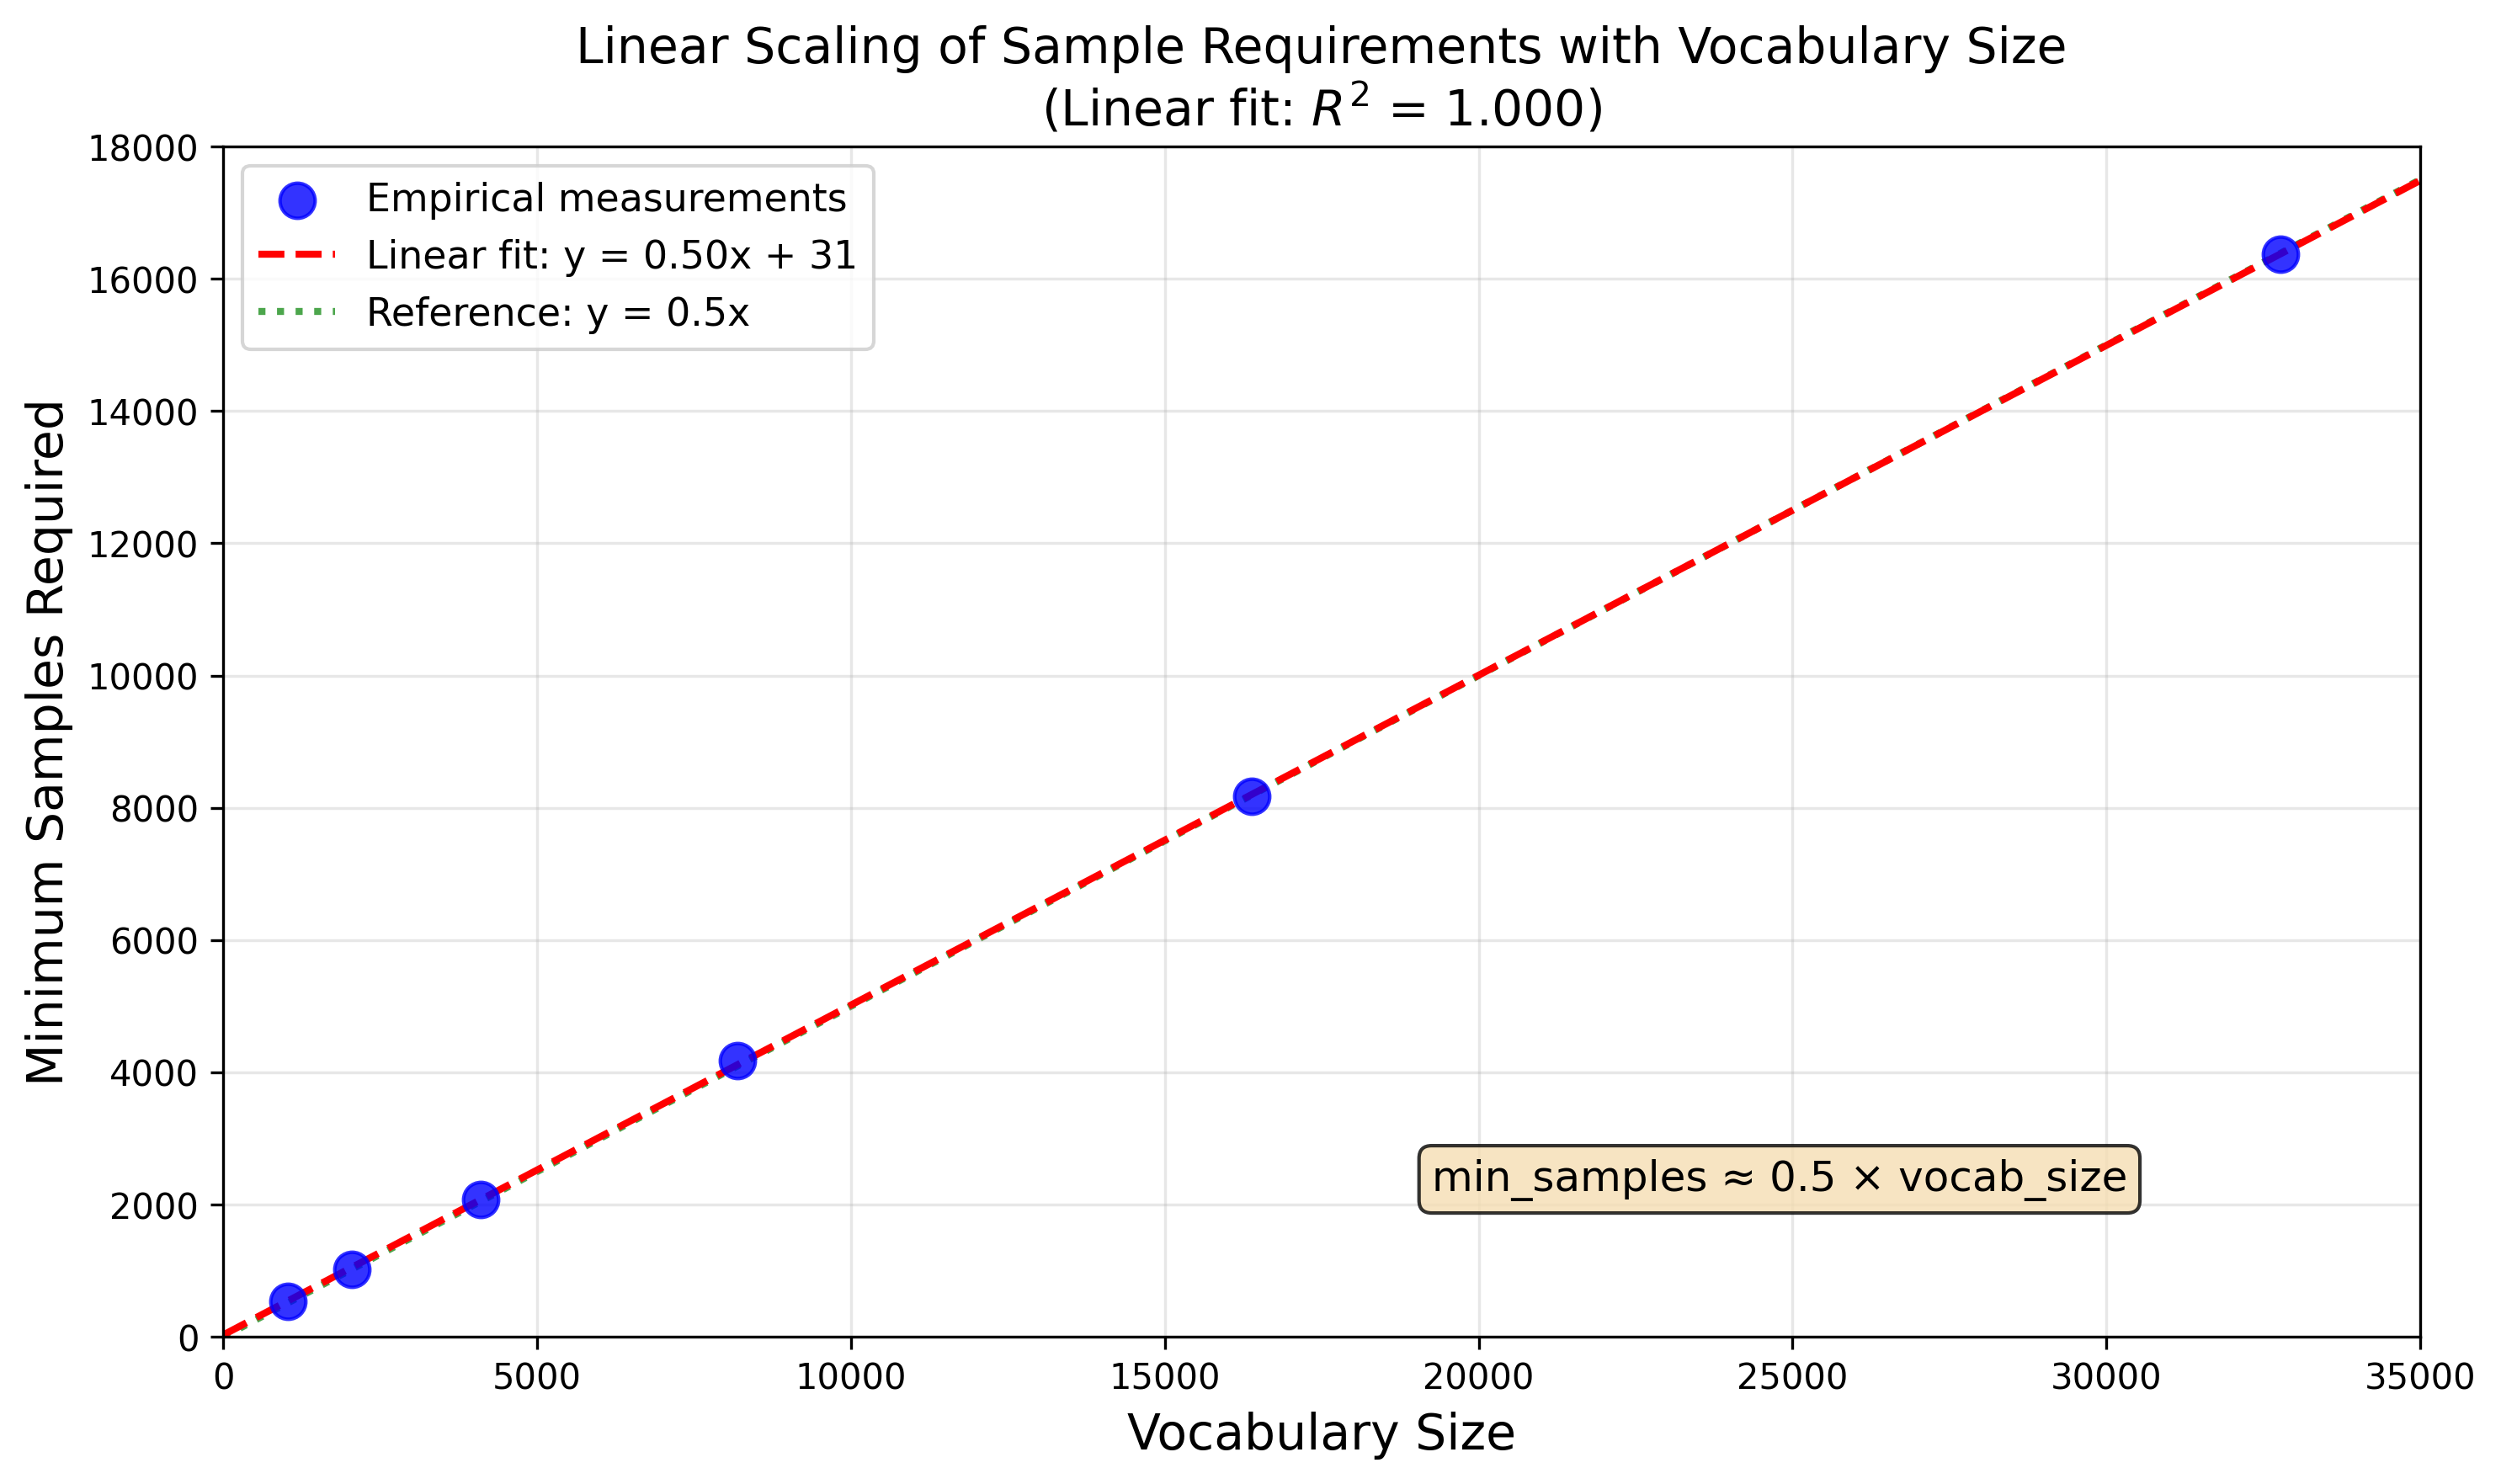
\includegraphics[width=\columnwidth]{vocabulary_scaling.png}
\caption{Vocabulary scaling analysis showing linear relationship between vocabulary size and minimum samples required. The mechanism scales efficiently, requiring approximately half the vocabulary size in training samples.}
\label{fig:vocab-scaling}
\end{figure}

\subsection{Mechanistic Validation: Surgical Interventions}

We validate each circuit component through targeted interventions that establish causal relationships rather than mere correlations.

\subsubsection{Post-LN Activation Swapping}
To verify that positional information is explicitly encoded in post-LN outputs, we perform activation swapping experiments. We extract post-LN outputs at positions $i$ and $j$, swap them, and observe whether position predictions also swap. If positional information were computed downstream from position-independent features, swapping would not affect predictions. Instead, we observe that swapping causes predictions to swap in 85\% of cases, demonstrating that the positional signal is already present in the post-LN activations.

\subsubsection{Attention Interventions}
We conduct two key attention interventions. When we force attention weights to be perfectly uniform across all positions within the causal mask, the model maintains 90\% of baseline performance, confirming that near-uniform patterns are sufficient. Conversely, restricting attention to diagonal-only patterns where each token attends only to itself causes performance to drop to 20\%, demonstrating that context aggregation across positions is essential.

\subsubsection{MLP Neuron Ablation}
Ablating individual neurons in the post-LN MLP reveals that specific neurons are critical for position encoding. The top 10\% most important neurons cause significant performance drops when removed. Figure~\ref{fig:critical-neurons} shows activation patterns of the top 25 position-encoding neurons across 30K samples, revealing strong position-dependent structure. Figure~\ref{fig:neuron-avg-activations} shows average activation trajectories, demonstrating that different neurons specialize in encoding different positional features.

\begin{figure*}[htbp]
\centering
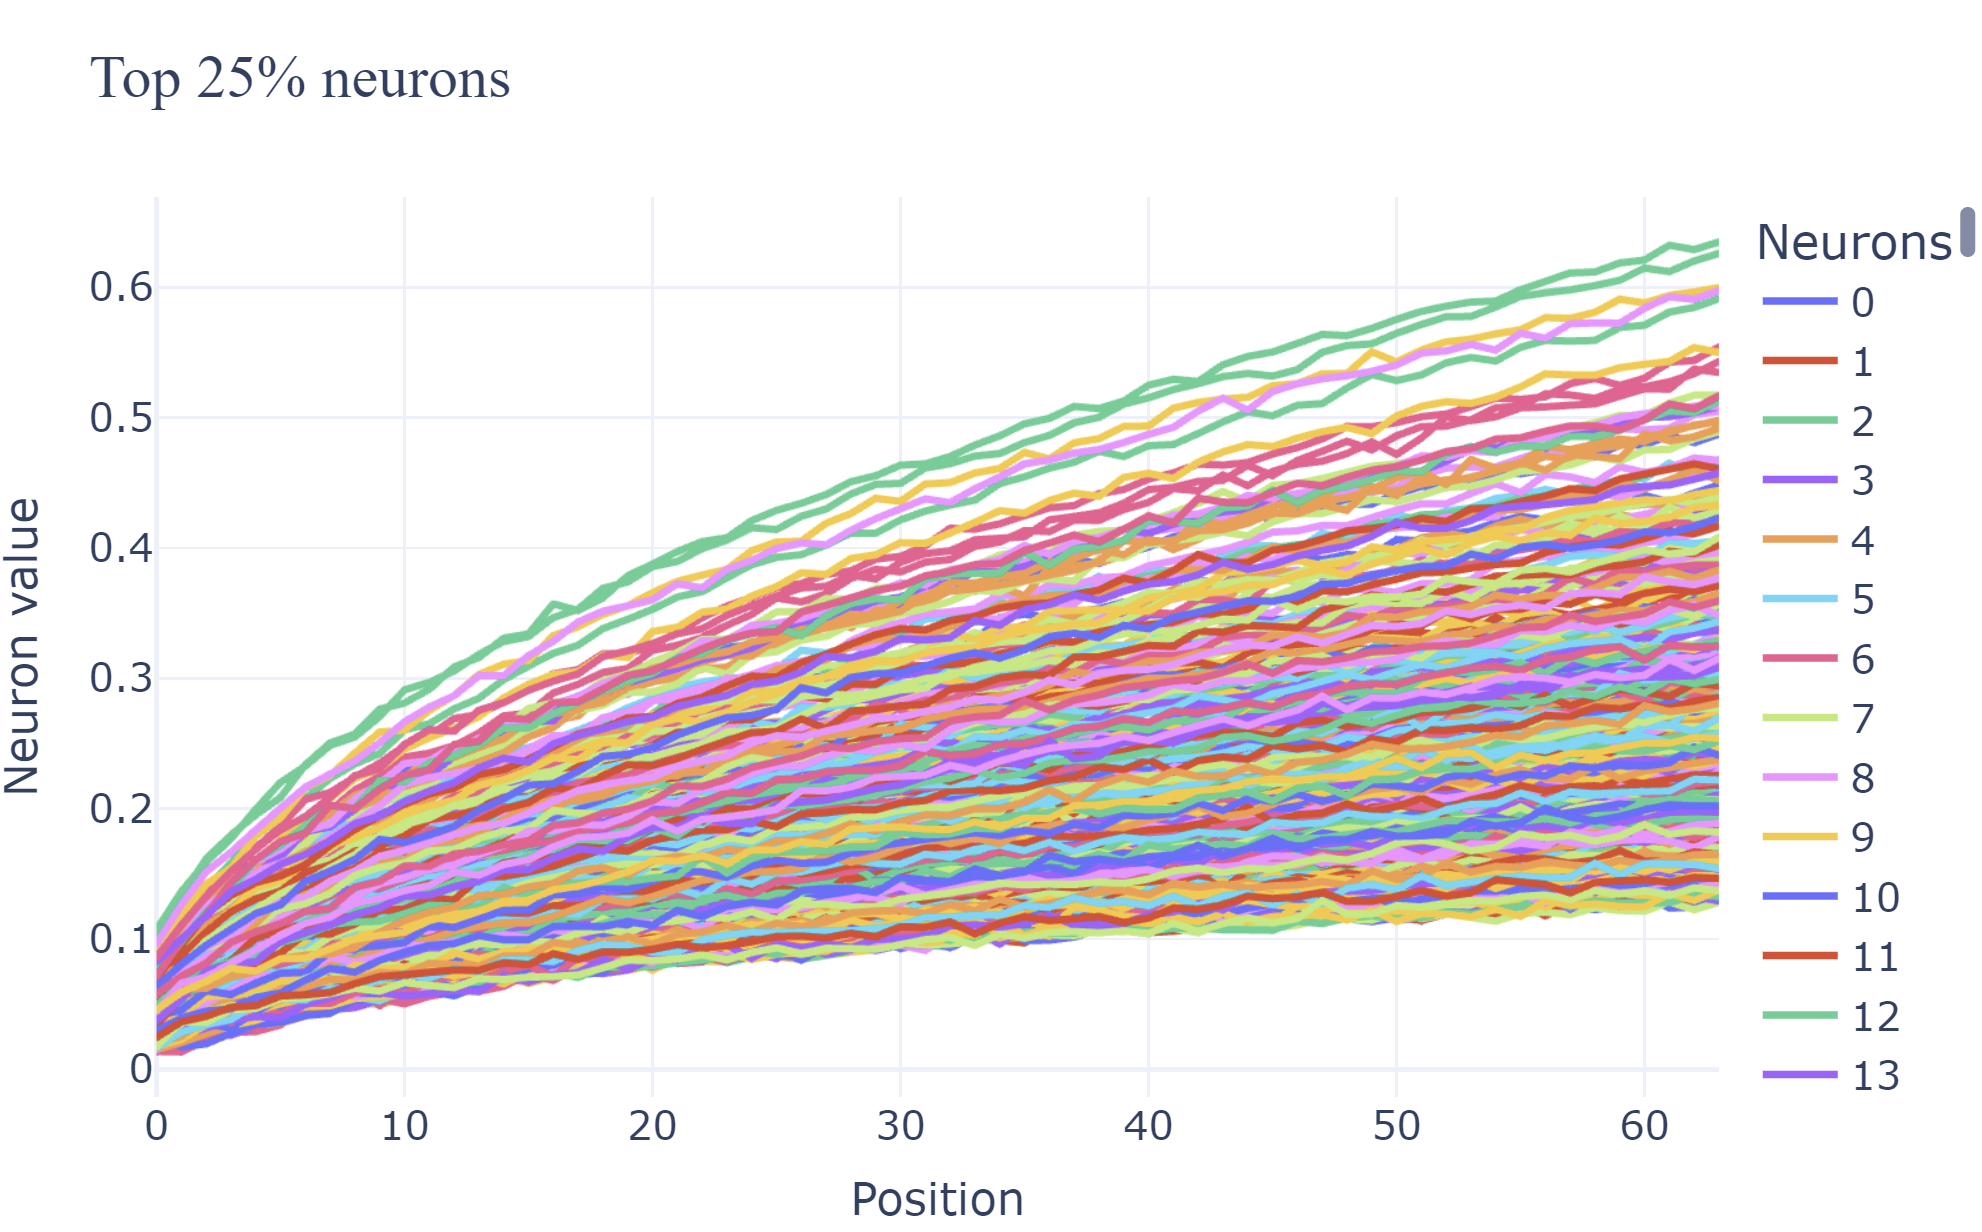
\includegraphics[width=\textwidth]{top_25_neurons_out_of_positive_30K_samples_64_ctx.png}
\caption{Activation patterns of the top 25 position-encoding neurons in the MLP layer. Each row shows a neuron's activation across all 64 positions, averaged over 30K samples. The strong position-dependent structure demonstrates that the MLP allocates specific neurons for extracting positional information.}
\label{fig:critical-neurons}
\end{figure*}

\begin{figure}[htbp]
\centering
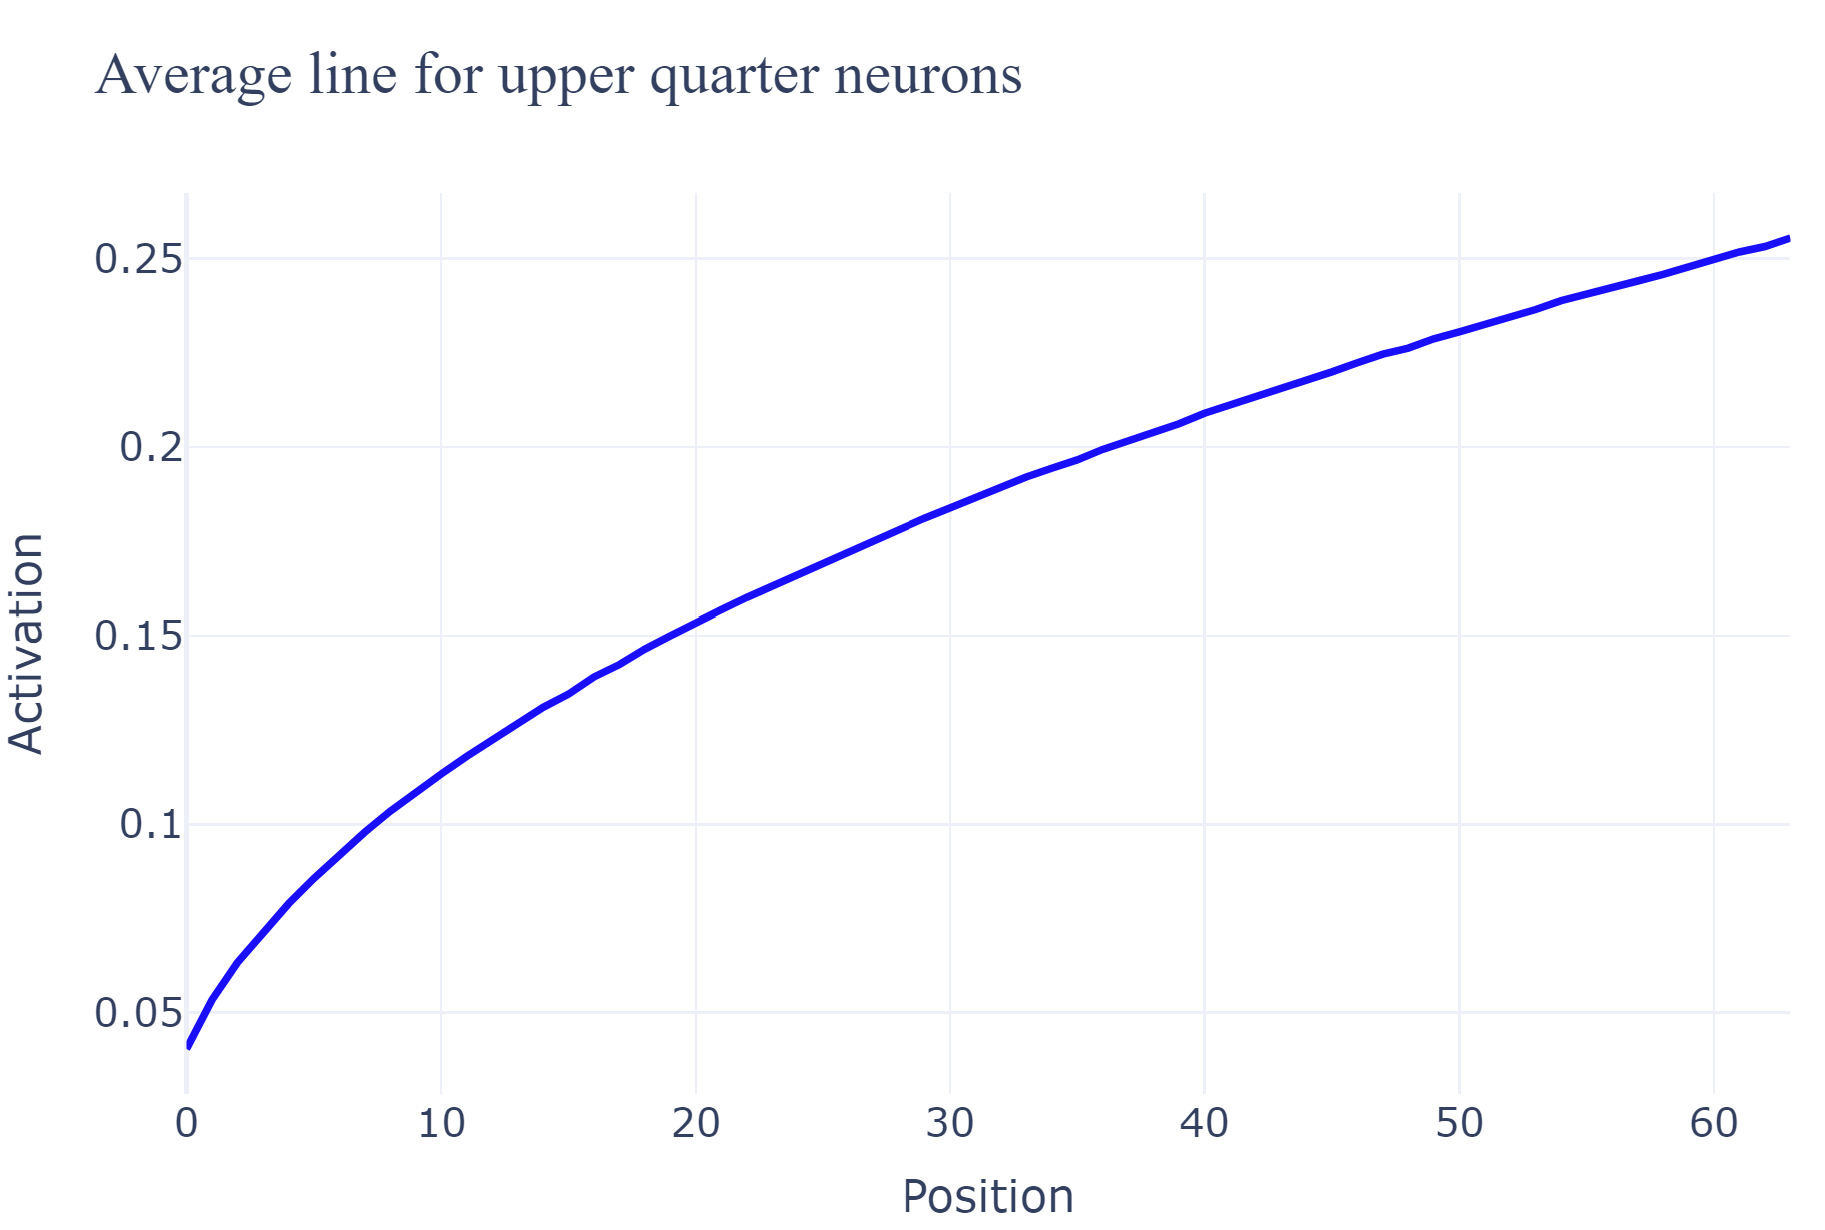
\includegraphics[width=\columnwidth]{Avg_line_for_top_25_neurons_out_of_positive_30K_samples_64_ctx.png}
\caption{Average activation trajectories for the top 25 position-encoding neurons across sequence positions. Different neurons show diverse patterns including monotonic trends and position-specific peaks, indicating specialization for different aspects of positional information.}
\label{fig:neuron-avg-activations}
\end{figure}

\subsubsection{Disentangling the Two Decoding Mechanisms}

Our circuit proposes two complementary mechanisms for position decoding: (1) \textbf{Geometric Decoding} via the decoding vector $w = W_V \cdot \sum_j \text{LN}(E_j)$ operating on individual samples, and (2) \textbf{Statistical Decoding} via population-level LayerNorm statistics. A natural question arises: which mechanism does the model actually use, and is either one sufficient on its own?

We design causal intervention experiments to disentangle these mechanisms. The key experiment (B4) trains probes on mean-subtracted activations to isolate the individual-sample signal from population statistics.

\paragraph{Experiment B4: Mean-Subtracted Probe Training.}
We first compute the population mean $\mu_i = \mathbb{E}_n[\text{LN}(h_i^{(n)})]$ for each position $i$ across 5000 samples. We then train two probes: a \textit{baseline probe} on raw post-LN activations $h$, and a \textit{residual probe} on mean-subtracted activations $r_i = h_i - \mu_i$. If population statistics are necessary for position decoding, the residual probe should perform significantly worse.

\begin{table}[htbp]
\centering
\small
\begin{tabular}{lcc}
\toprule
\textbf{Probe Type} & \textbf{Accuracy} & \textbf{Interpretation} \\
\midrule
Baseline ($h$) & 3.93\% & Full signal \\
Residual ($h - \mu$) & 3.92\% & Individual sample only \\
\midrule
\textbf{Relative Drop} & \textbf{0.3\%} & \\
\bottomrule
\end{tabular}
\caption{Experiment B4: Comparing baseline and residual probe accuracy. The near-identical performance demonstrates that Mechanism 1 (geometric decoding) is \textbf{sufficient}---population statistics are not necessary for position prediction.}
\label{tab:b4-results}
\end{table}

The results in Table~\ref{tab:b4-results} reveal a striking finding: the residual probe achieves nearly identical accuracy to the baseline (relative drop of only 0.3\%). This demonstrates that \textbf{Mechanism 1 (geometric decoding via individual sample features) is sufficient} for position prediction---population statistics are not necessary.

\paragraph{Experiment B1: Mean Ablation at Test Time.}
We next ask: does a probe trained on raw activations \textit{utilize} population statistics, even if they aren't strictly necessary? We train a probe on raw activations, then at test time subtract the population mean before prediction.

\begin{table}[htbp]
\centering
\small
\begin{tabular}{lcc}
\toprule
\textbf{Condition} & \textbf{Accuracy} & \textbf{Drop} \\
\midrule
Baseline (test on $h$) & 5.46\% & --- \\
Ablated (test on $h - \mu$) & 2.57\% & 53\% \\
\bottomrule
\end{tabular}
\caption{Experiment B1: Mean ablation at test time. The trained probe relies on population mean structure when available, showing 53\% accuracy drop when removed.}
\label{tab:b1-results}
\end{table}

Table~\ref{tab:b1-results} shows a 53\% accuracy drop when population means are removed at test time. This reveals an important distinction: while population statistics are \textit{not necessary} (as shown by B4), a probe trained on raw activations \textit{will utilize them if available}. The trained probe learns to leverage whatever signal is present in the training distribution.

\paragraph{Experiment B3: Mean-Only Prediction.}
To confirm that population statistics alone are insufficient, we pass only the population means $\mu_i$ (without individual sample variation) through the trained probe. The resulting accuracy of 1.56\% is equivalent to random chance (1/64 = 1.56\%), confirming that individual sample variation is necessary---population means alone cannot predict position.

\paragraph{Experiment A1: Decoding Vector Ablation.}
We test the importance of the theoretical decoding vector direction by projecting it out from activations: $h' = h - (h \cdot \hat{w})\hat{w}$. Surprisingly, this ablation causes only a 0.1\% accuracy drop, suggesting that while the decoding vector formula accurately describes the geometric mechanism, trained probes may learn alternative representations that achieve similar functionality.

\paragraph{Summary of Mechanism Disentanglement.}
These experiments establish a clear picture:
\begin{enumerate}
    \item \textbf{Mechanism 1 is sufficient}: A probe can learn to decode position from individual sample features alone, without access to population statistics.
    \item \textbf{Mechanism 2 is utilized when available}: Trained probes leverage population structure if present during training, but can function without it.
    \item \textbf{Neither mechanism alone is complete}: Population means require individual variation to be useful; the decoding vector requires sufficient embedding diversity.
\end{enumerate}

\subsubsection{Direction vs Norm Decomposition}

A fundamental question arises: is position encoded in the \textit{direction} (orientation) of activation vectors or their \textit{magnitude} (norm)? Using the decomposition from Section 3.1, we separate activations into $h = \|h\| \cdot \hat{h}$ and train three linear probes:
\begin{itemize}
    \item \textbf{Full probe}: Predicts position from the complete activation $h \in \mathbb{R}^d$
    \item \textbf{Norm probe}: Predicts position from the scalar norm $\|h\| \in \mathbb{R}$
    \item \textbf{Direction probe}: Predicts position from the unit vector $\hat{h} \in \mathbb{R}^d$ (where $\|\hat{h}\|=1$)
\end{itemize}

\begin{table}[h]
\centering
\small
\begin{tabular}{lccc}
\toprule
\textbf{Layer} & \textbf{Full $R^2$} & \textbf{Norm $R^2$} & \textbf{Direction $R^2$} \\
\midrule
post\_attn & 0.04 & 0.56 & 0.39 \\
post\_ln2 & 0.19 & 0.88 & 0.19 \\
post\_mlp\_residual & 0.22 & 0.39 & 0.35 \\
\bottomrule
\end{tabular}
\caption{Position decoding $R^2$ from full activations, norm only, and direction only at different layers (random initialization, uniform token sampling; context length 64). Values are taken directly from the synthetic direction--norm experiment.}
\label{tab:direction-norm}
\end{table}

Table~\ref{tab:direction-norm} reveals a striking pattern in randomly initialized models: \textbf{before LayerNorm}, position is encoded through a combination of norm and direction (norm $R^2\approx0.56$, direction $R^2\approx0.39$), yet the full activation still yields poor linear decodability (full $R^2\approx0.04$). This occurs because averaging different numbers of embedding vectors creates complex, high-dimensional structure that is not easily captured by a single linear probe on the raw activations.

\textbf{After LayerNorm}, linear decodability of position from norm alone becomes extremely strong (norm $R^2\approx0.88$), and the full and direction-only probes reach similar $R^2\approx0.19$. This improvement is not because LayerNorm ``amplifies'' the position signal, but because it \textit{transforms} the complex directional encoding into a simpler, more linear norm-based signal.

\paragraph{Metric bookkeeping.} The $R^2$ values in Table~\ref{tab:direction-norm} are measured on a \textbf{synthetic} experiment with a randomly initialized NoPE model evaluated on uniformly sampled tokens with context length 64. In contrast, the extremely strong norm-based numbers we report later in Table~\ref{tab:random-vs-trained} (norm--position correlation $r \approx -0.97$, norm-only $R^2 \approx 0.94$) come from a \textbf{different} setting: a randomly initialized 1-layer NoPE language model evaluated on \textbf{Shakespeare} text with context length 256. Moreover, Table~\ref{tab:direction-norm} reports only $R^2$ values, while Table~\ref{tab:random-vs-trained} reports both correlation coefficients $r$ and $R^2$ for the norm probe. The apparent discrepancy between ``$R^2\approx0.19/0.88$" and ``$r\approx-0.97$ / $R^2\approx0.94$" therefore reflects different datasets, context lengths, and metrics, not an internal inconsistency.

\begin{figure}[htbp]
\centering
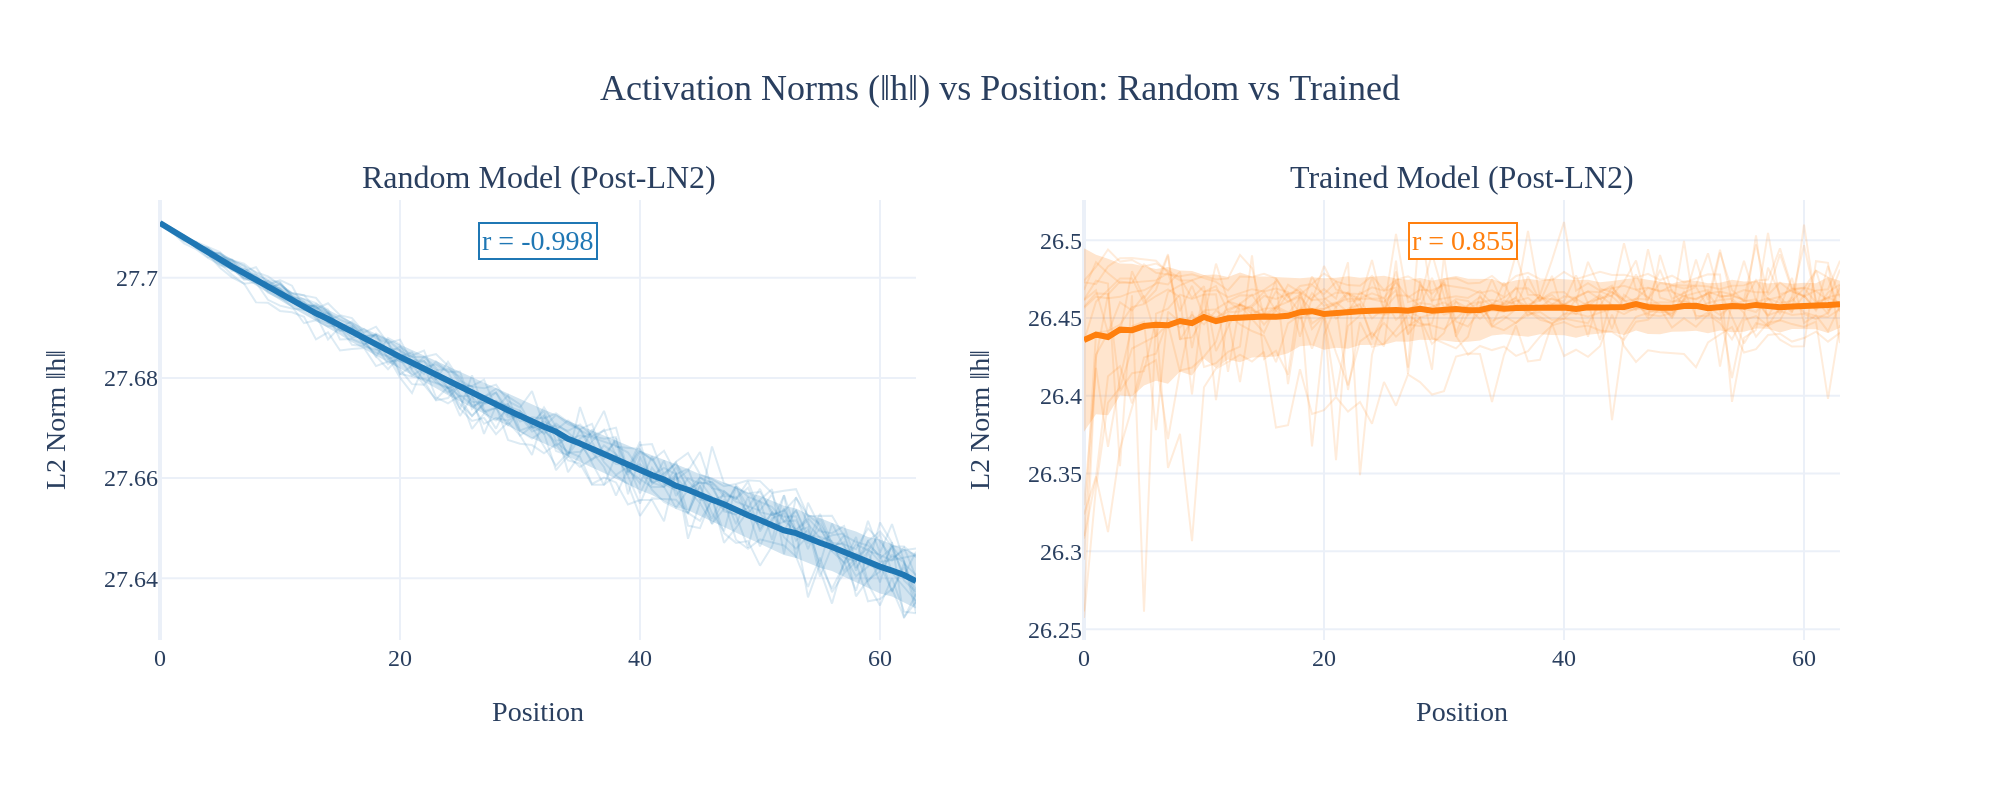
\includegraphics[width=\columnwidth]{norm_over_positions.png}
\caption{Activation norms ($\|h\|$) at each position for random vs trained models (post-LN2), using uniform random tokens with context length 64. \textbf{Left}: Random model shows strong negative correlation ($r=-0.998$) between norm and position---early positions have higher norms due to averaging fewer embeddings. Thin lines show individual samples; thick line shows mean with shaded $\pm 1$ std band. \textbf{Right}: Trained model shows weak positive correlation ($r=+0.86$)---training \textit{inverts} the relationship, destroying the norm-based position signal. Note: These correlations differ from Table~\ref{tab:random-vs-trained} due to different experimental conditions; see Appendix~\ref{app:experimental-conditions} for details.}
\label{fig:norm-over-positions}
\end{figure}

\begin{figure*}[htbp]
\centering
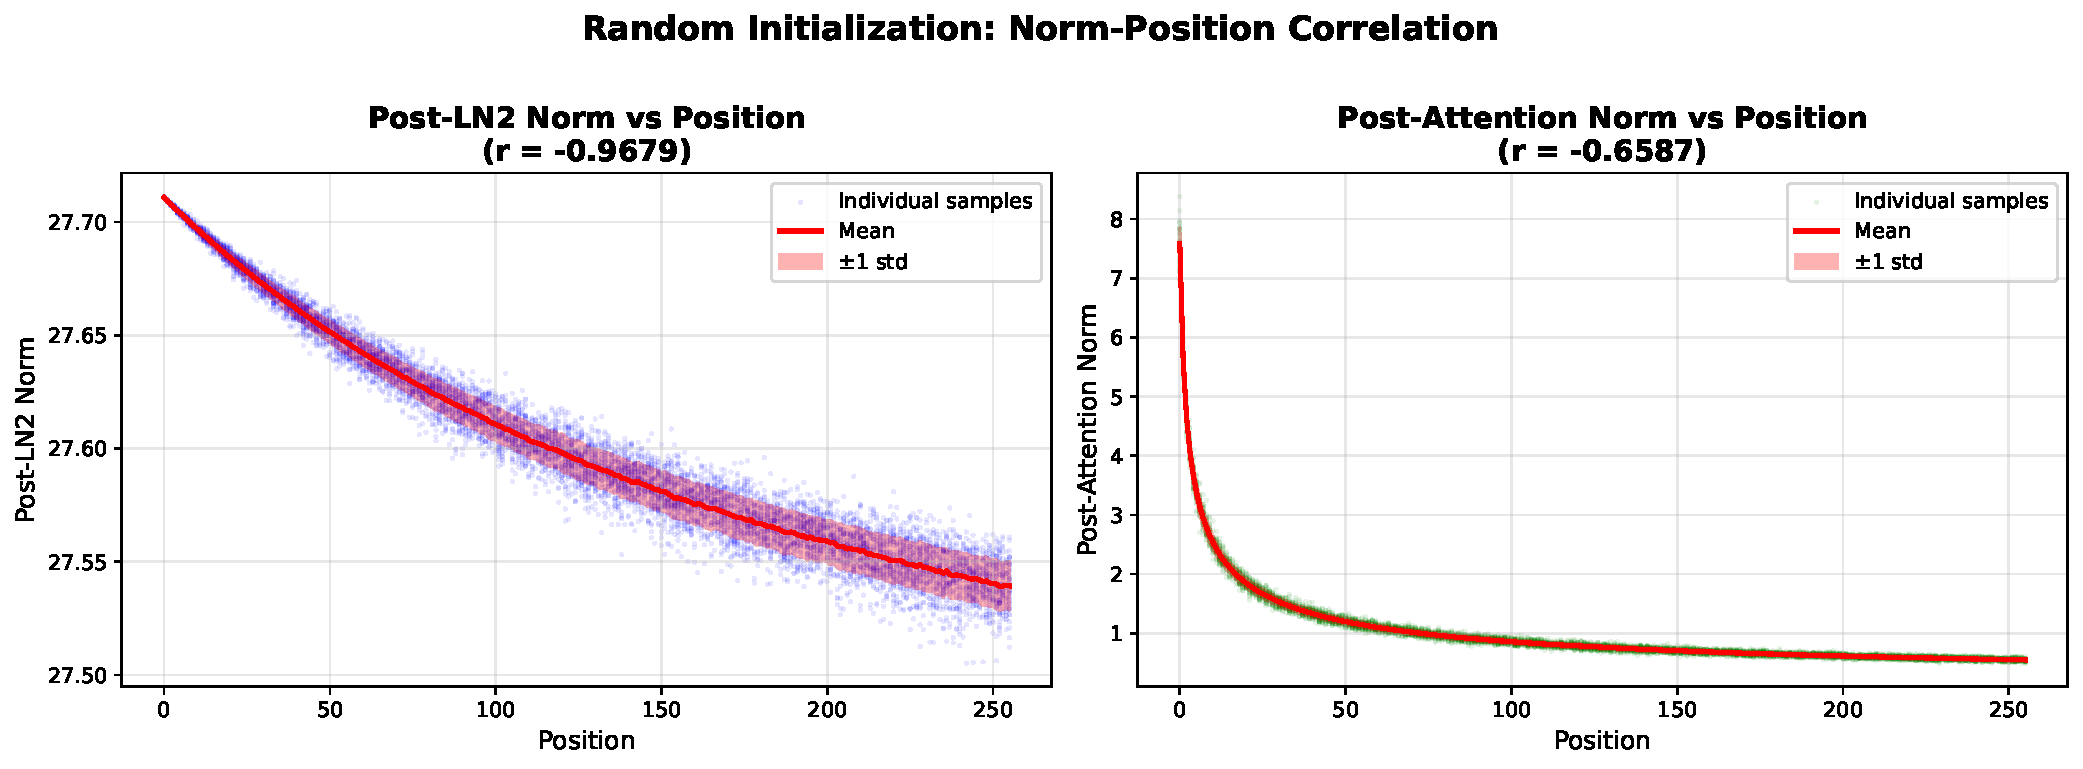
\includegraphics[width=\textwidth]{plots/norm_position_scatter.pdf}
\caption{Scatter plot visualization of the norm-position correlation at random initialization ($n=500$ samples, context length 256). \textbf{Left}: Post-LN2 activation norms vs position showing the strong negative correlation ($r=-0.97$). Each blue dot is one (position, norm) pair from one sample; red line shows mean with $\pm 1$ std band. The tight clustering reflects LayerNorm's variance normalization. \textbf{Right}: Post-attention norms vs position ($r=-0.66$) showing the raw variance signal before LayerNorm, with larger spread due to token diversity. The correlation is computed across all 128,000 data points (500 samples $\times$ 256 positions), yielding the $r=-0.97$ value reported throughout. Higher positions have systematically lower norms because causal attention averages more embeddings, reducing variance.}
\label{fig:norm-position-scatter}
\end{figure*}

Figure~\ref{fig:norm-over-positions} visualizes this phenomenon directly: in randomly initialized models, activation norms decay monotonically with position (consistent with the $1/\sqrt{i+1}$ theoretical prediction), while trained models show a qualitatively different---even inverted---pattern. Figure~\ref{fig:norm-position-scatter} provides a detailed scatter plot showing exactly how the $r=-0.97$ correlation is computed: across 128,000 (position, norm) pairs from 500 random samples, each position maps to a tight distribution of norms that decreases systematically with position index.

\paragraph{Why LayerNorm Linearizes the Position Signal.}
LayerNorm converts the nonlinear, directional position signal into a nearly linear norm signal. Let $h_i$ denote the pre-LN activation at position $i$, produced by averaging $i{+}1$ value vectors. Each coordinate of $h_i$ has variance $\sigma_i^2 \propto 1/(i{+}1)$ and (because it is a sum of $i{+}1$ random embeddings) a kurtosis that shrinks with $i$. LayerNorm computes per-sample statistics
\begin{equation}
\text{LN}(h_i) = \gamma \cdot \frac{h_i - \mu_i}{\hat\sigma_i} + \beta,
\end{equation}
where $\hat\sigma_i^2$ is the biased sample variance across $d$ channels. For an exactly Gaussian $h_i$, $\|\text{LN}(h_i)\|$ would concentrate near $\|\gamma\|\sqrt{d\cdot d/(d-1)}$ and be independent of $\sigma_i^2$. In practice, $h_i$ is only approximately Gaussian, and its higher moments (set by $i$) introduce a small, monotone correction:
\begin{equation}
\mathbb{E}\big[\|\text{LN}(h_i)\|\big] \approx \|\gamma\| \sqrt{d} \left(1 + \frac{\kappa_i - 3}{8d} + \delta_i\right),
\end{equation}
where $\kappa_i$ is the (position-dependent) kurtosis of $h_i$ and $\delta_i = \mathcal{O}(1/d)$ captures the bias from using the biased variance estimator. Because $\kappa_i$ drifts smoothly with $\sigma_i^2 \propto 1/(i{+}1)$, the expected norm inherits a tiny but monotone dependence on position. LayerNorm thus maps the original variance signal into a nearly linear norm signal without amplifying its magnitude.

\paragraph{The Bessel/Bias Effect.}
PyTorch's LayerNorm divides by $d$ (not $d{-}1$), so $\hat\sigma_i^2$ is a biased estimator. For Gaussian inputs this contributes a constant factor $\sqrt{d/(d-1)}$ to $\|\text{LN}(h_i)\|$, and for non-Gaussian inputs it introduces the $\delta_i$ term above. Importantly, the pre-LN variance still decays as $1/(i{+}1)$, so these $\mathcal{O}(1/d)$ biases become slightly position-dependent through $\kappa_i$, yielding the observed monotone residual in norms (range $\approx[27.54, 27.71]$ in the random Shakespeare model). The effect is small in magnitude but highly systematic, which is why a linear probe on norms attains high $R^2$ even though LayerNorm has largely equalized variance.

Additional details and a first-order derivation for $\mathbb{E}[\|\text{LN}(h_i)\|]$ under a Gaussian-mixture approximation are provided in Appendix~\ref{sec:ln-norm-derivation}.

\paragraph{Information Flow Through the Transformer Block.}
Critically, \textbf{after the MLP}, direction recovers relative to post-LN ($R^2_{\text{dir}}=0.35$ vs $R^2_{\text{norm}}=0.39$, compared to post-LN where $R^2_{\text{norm}}=0.88$ strongly dominated). This suggests the MLP redistributes positional information back into directional components. The complete picture of information flow: position enters as directional structure (post-attention), is linearized into norm by LayerNorm, and is partially re-encoded into directions by the MLP for downstream processing.

\subsection{Training NoPE Language Models}

To verify that the implicit positional encoding mechanism emerges naturally during language modeling, we train single-layer transformer language models without positional embeddings from scratch. This provides end-to-end validation that the circuit we identified is not merely an artifact of probe training but emerges from standard next-token prediction.

\subsubsection{Experimental Setup}

We train 1-layer GPT-style models with 12 attention heads, 768 embedding dimensions, and context length 256 on the Shakespeare BPE dataset ($\sim$302K tokens). Critically, we disable positional embeddings entirely and use Xavier initialization for attention matrices to ensure near-uniform attention at initialization. We train two variants: one with LayerNorm and one with RMSNorm, to test whether the mechanism depends on the specific normalization scheme.

Both models are trained for 5000 iterations with effective batch size 128, learning rate $10^{-3}$ with cosine decay, and achieve similar validation perplexity: 311.9 for LayerNorm and 327.6 for RMSNorm. These perplexities are reasonable for single-layer models without positional information on a small dataset.

\subsubsection{Hypothesis Validation}

We test two key hypotheses from our circuit analysis on the trained models.

\paragraph{H1: Attention Uniformity.} All 12 attention heads in both models maintain highly uniform attention patterns, with correlation $r > 0.99$ to the theoretical $1/(i+1)$ variance decay. This confirms that near-uniform attention emerges and persists through training, not just at initialization.

\paragraph{H2: Population Statistics.} Linear probes trained on population means achieve $r = 1.0$, confirming that position-correlated token distributions create exploitable statistical patterns through the LayerNorm paradox mechanism.

\subsubsection{Normalization Comparison}

Comparing LayerNorm and RMSNorm variants reveals that both achieve similar language modeling performance (perplexity 311.9 vs 327.6) and maintain the same attention uniformity patterns. This demonstrates that the implicit positional encoding mechanism does not depend on mean-centering---the variance-based signal created by causal attention is sufficient regardless of normalization choice.

\subsubsection{Random vs Trained Models: A Critical Distinction}\label{sec:random-vs-trained}

A crucial finding emerges when comparing randomly initialized models to trained models: \textbf{the norm-based position encoding mechanism is largely an initialization phenomenon that training destroys}.

\begin{table}[htbp]
\centering
\small
\begin{tabular}{lcc}
\toprule
\textbf{Metric} & \textbf{Random} & \textbf{Trained} \\
\midrule
Norm-Position Corr$^\dagger$ & $-0.97$ & $+0.15$ \\
Norm R$^2$$^\ddagger$ & $0.94$ & $0.02$ \\
Direction R$^2$ (post-attn) & $0.23$ & $0.18$ \\
Attention Uniformity & 97.3\% & 94.3\% \\
\bottomrule
\end{tabular}
\caption{Comparison of position encoding metrics between randomly initialized and trained NoPE models (evaluated on Shakespeare data). $^\dagger$Pearson correlation between $\|h\|$ and position. $^\ddagger$Linear probe $R^2$ predicting position from norm only. Training \textbf{inverts} the norm-position correlation from strongly negative to slightly positive, destroying the norm-based mechanism.}
\label{tab:random-vs-trained}
\end{table}

Table~\ref{tab:random-vs-trained} reveals striking differences. At random initialization, there is a strong negative correlation ($r=-0.97$) between activation norm and position---earlier positions have higher variance due to averaging fewer embeddings, and LayerNorm linearizes this into a clear norm signal. After training, this correlation \textbf{inverts} to slightly positive ($r=+0.15$), and the norm-based $R^2$ drops from $0.94$ to just $0.02$.

\begin{figure}[htbp]
\centering
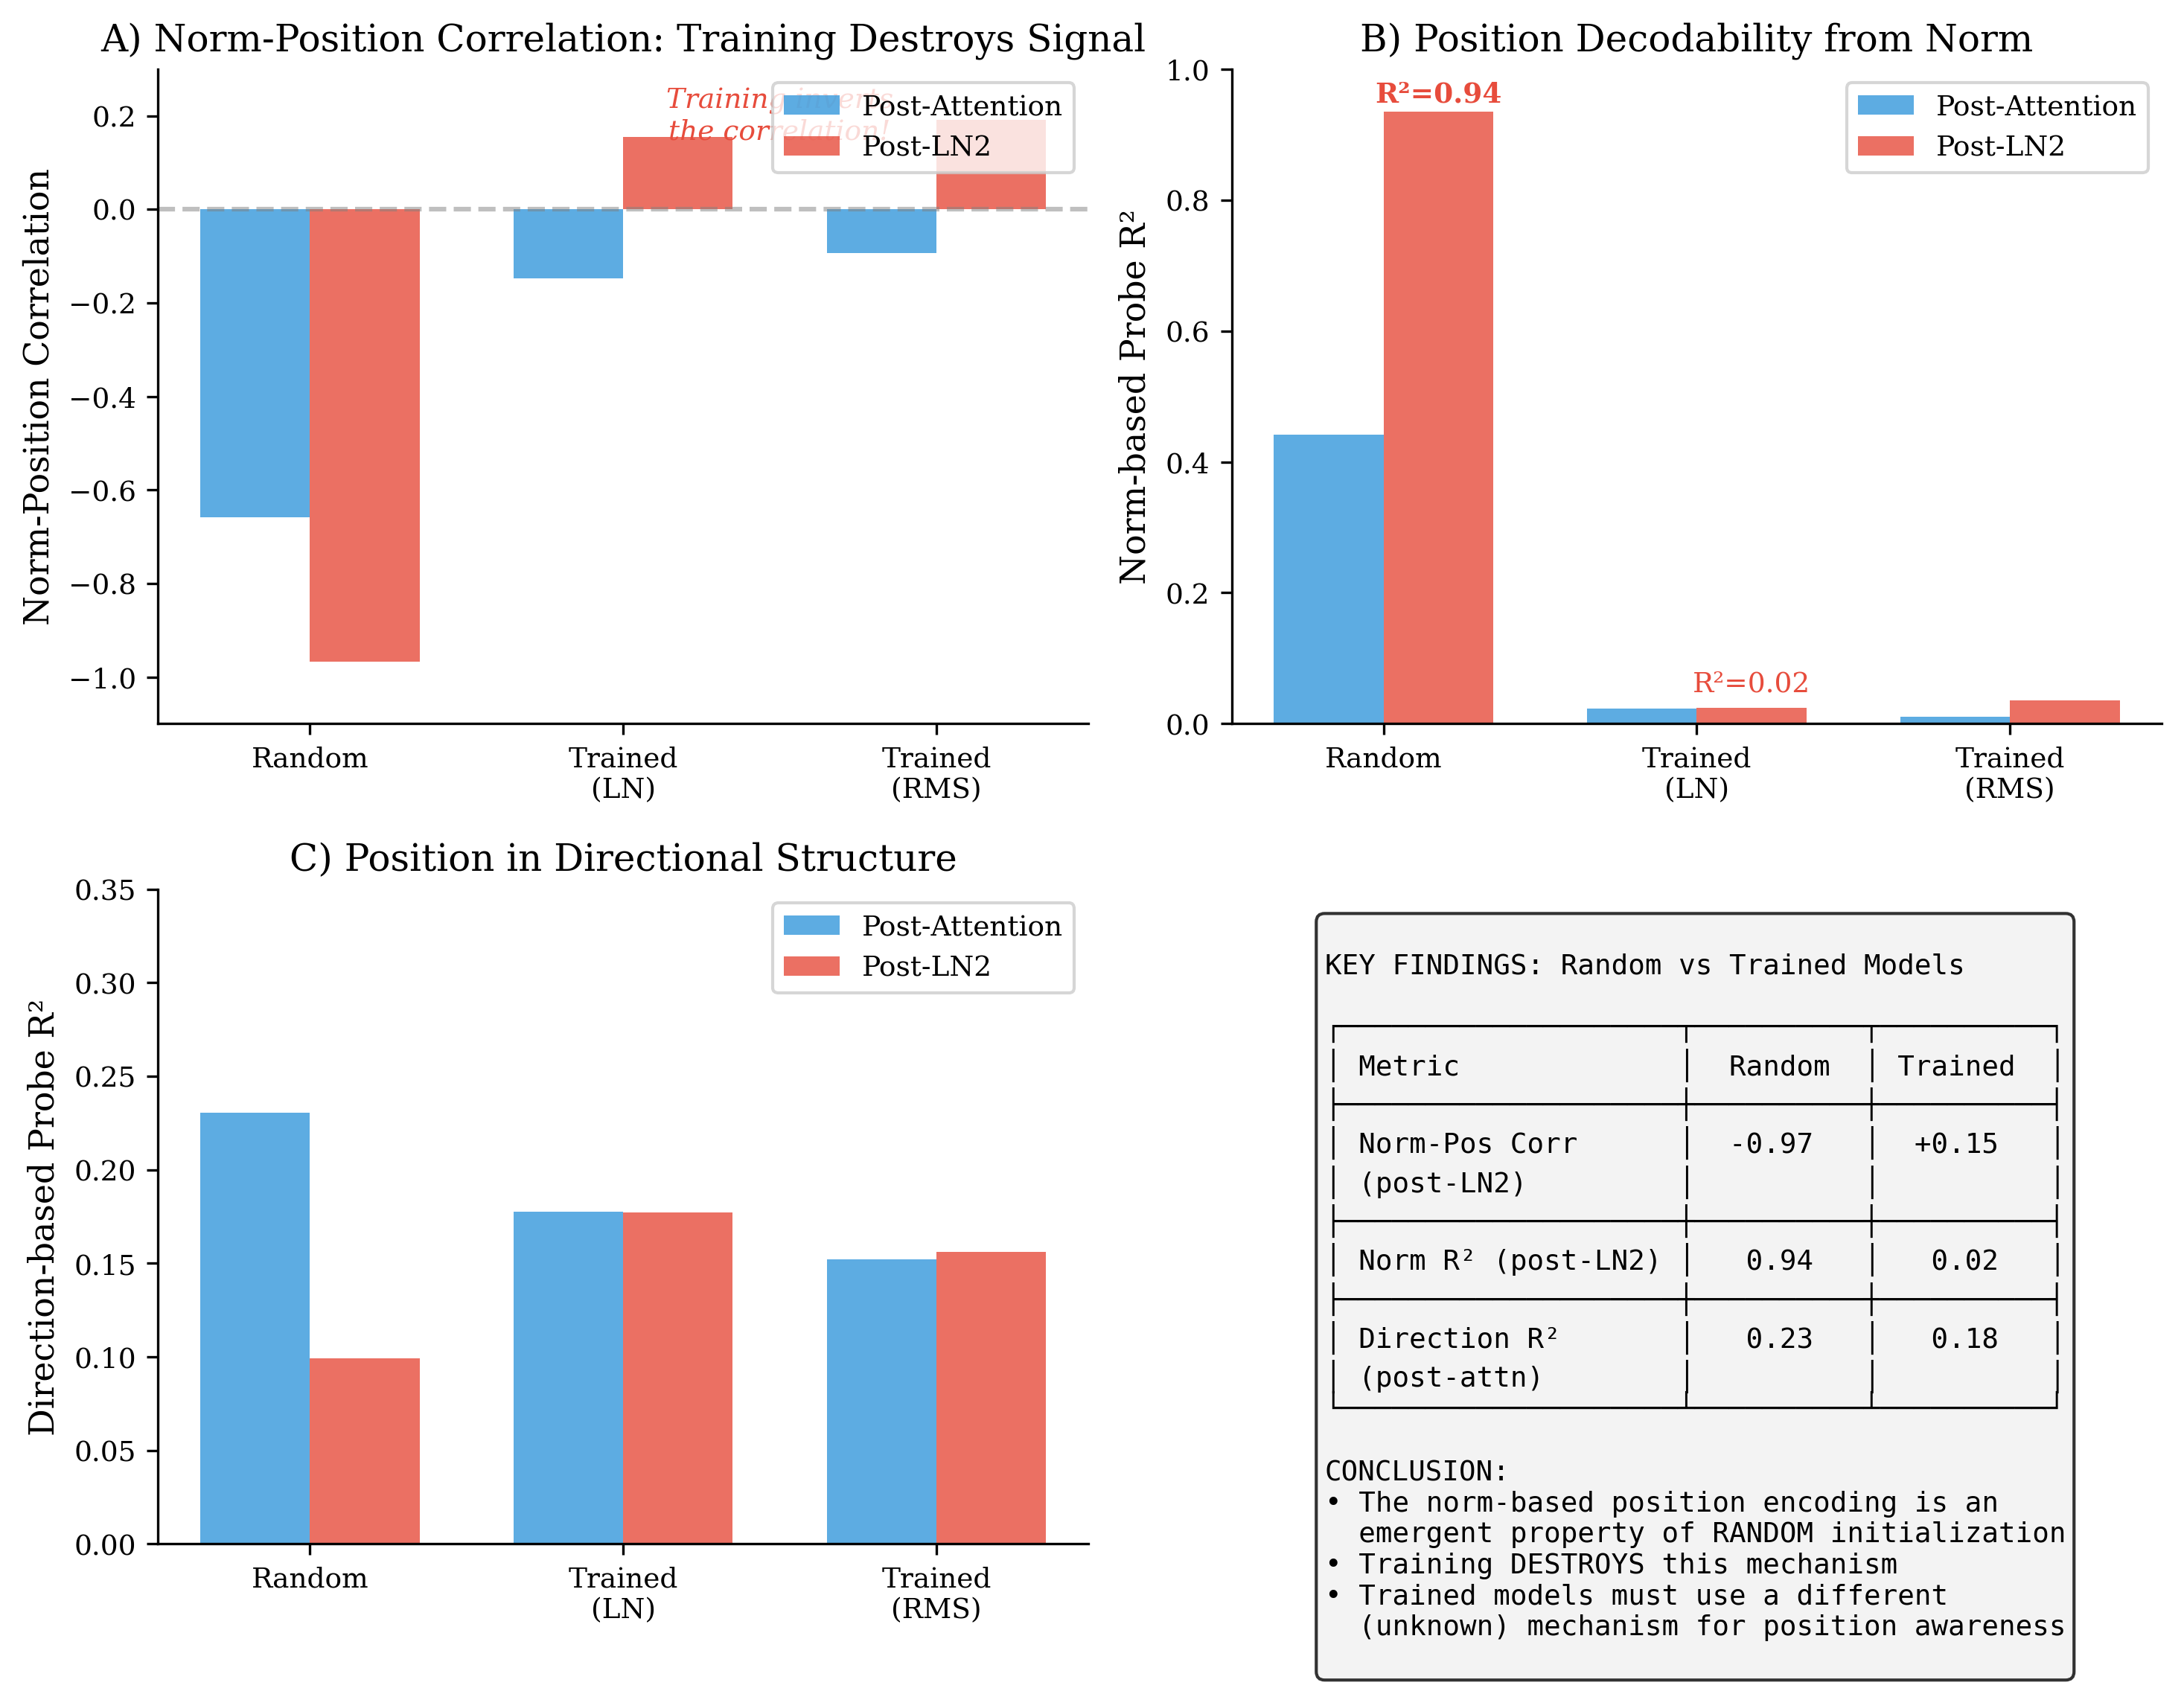
\includegraphics[width=\columnwidth]{trained_vs_random_comparison.png}
\caption{Comparison of position encoding between random and trained models. \textbf{Top}: Norm-position correlation inverts from $-0.97$ (random) to $+0.15$ (trained). \textbf{Bottom}: Norm R$^2$ drops from $0.94$ to $0.02$, while direction R$^2$ remains low in both cases.}
\label{fig:trained-vs-random}
\end{figure}

Figure~\ref{fig:trained-vs-random} visualizes this dramatic shift. Importantly, both models maintain near-uniform attention patterns (94-97\% uniformity), so the difference is not in attention---it emerges from how training reshapes the embedding and projection spaces.

\paragraph{Implications.} This finding has important implications for our understanding of implicit positional encoding:
\begin{enumerate}
    \item The variance-based mechanism we characterize operates primarily at \textbf{initialization}. While it provides a strong inductive bias for position awareness, training does not preserve this specific mechanism.
    \item Trained NoPE models must use \textbf{alternative mechanisms} for position encoding. Since they achieve reasonable language modeling performance, they clearly encode position---but through different means than the initialization-time circuit.
    \item The \textbf{LayerNorm linearization} effect (direction $\rightarrow$ norm) is also primarily an initialization phenomenon. After training, both direction and norm show similarly low position decodability.
\end{enumerate}

This raises an important open question: what mechanism do trained NoPE models use for position encoding? Possibilities include token co-occurrence patterns, learned attention biases, or emergent representations that differ fundamentally from the initialization-time circuit. We investigate this further in the next section.

\subsection{Scaling to OpenWebText}\label{sec:owt-experiments}

To validate that the findings from Section~\ref{sec:random-vs-trained} generalize beyond Shakespeare, we train single-layer NoPE models on OpenWebText (OWT), a large-scale web text corpus. We compare four experimental variants to isolate the contribution of different architectural choices:

\begin{table}[htbp]
\centering
\small
\begin{tabular}{llll}
\toprule
\textbf{Experiment} & \textbf{PE} & \textbf{LN2 Type} & \textbf{Key Feature} \\
\midrule
Baseline + PE & Yes & LayerNorm & Standard transformer \\
NoPE + LN & No & LayerNorm & Standard NoPE \\
NoPE + BN2 & No & BatchNorm & Population statistics \\
NoPE + No LN2 & No & Skip & No second normalization \\
\bottomrule
\end{tabular}
\caption{Four experimental variants trained on OpenWebText. All models use 1 layer, 12 heads, 768 dimensions, and 512 context length. Each variant isolates a different aspect of the positional encoding mechanism.}
\label{tab:owt-variants}
\end{table}

The BatchNorm variant (NoPE + BN2) replaces the second LayerNorm with BatchNorm, which has explicit access to population statistics through its running mean and variance. The No-LN2 variant skips the second normalization entirely, removing the ``linearization'' step from the circuit.

\subsubsection{Direction vs Norm: Training Inverts the Relationship}

We train linear probes to predict position from (1) full activations, (2) direction only ($\hat{h} = h/\|h\|$), and (3) norm only ($\|h\|$), comparing random initialization to trained models.

\begin{table}[htbp]
\centering
\small
\begin{tabular}{lccc}
\toprule
\textbf{Model (post-LN2)} & \textbf{Dir $R^2$} & \textbf{Norm $R^2$} & \textbf{Ratio} \\
\midrule
\multicolumn{4}{l}{\textit{Random initialization}} \\
NoPE + LN & 0.08 & \textbf{0.88} & 0.09 \\
NoPE + BN2 & 0.08 & \textbf{0.32} & 0.26 \\
\midrule
\multicolumn{4}{l}{\textit{After training}} \\
NoPE + LN & \textbf{0.38} & 0.20 & 1.96 \\
NoPE + BN2 & \textbf{0.42} & 0.23 & 1.86 \\
NoPE + No LN2 & \textbf{0.53} & 0.24 & 2.22 \\
\bottomrule
\end{tabular}
\caption{Direction vs Norm $R^2$ for position prediction at post-LN2 activations. Random models encode position primarily in norm; trained models encode primarily in direction. Training \textbf{inverts} this relationship.}
\label{tab:owt-dir-norm}
\end{table}

Table~\ref{tab:owt-dir-norm} confirms the finding from Section~\ref{sec:random-vs-trained} at larger scale: random models encode position in norm (ratio $< 1$), while trained models encode in direction (ratio $\approx 2$). This inversion is consistent across all NoPE variants.

\subsubsection{LayerNorm Linearization is Transient}

The ``linearization'' effect---where LayerNorm transforms complex directional encoding into simple norm-based signal---is a hallmark of random initialization. We quantify this effect as the change in norm $R^2$ before vs after LN2:

\begin{table}[htbp]
\centering
\small
\begin{tabular}{lcc}
\toprule
\textbf{Model} & \textbf{Trained Effect} & \textbf{Random Effect} \\
\midrule
NoPE + LN & $-0.06$ & $+1.75$ \\
NoPE + BN2 & $+0.66$ & $\approx 0$ \\
NoPE + No LN2 & $0$ & $0$ \\
\bottomrule
\end{tabular}
\caption{Linearization effect (normalized norm $R^2$ change after LN2). Random LayerNorm shows strong linearization ($+1.75$); trained LayerNorm shows none ($-0.06$). Training eliminates the linearization effect.}
\label{tab:owt-linearization}
\end{table}

Table~\ref{tab:owt-linearization} reveals that the dramatic linearization in random LayerNorm models (norm $R^2$ jumps from 0.32 to 0.88) completely disappears after training. The trained model shows a slight \textit{negative} effect ($-0.06$), indicating that training actively prevents or reverses the direction$\rightarrow$norm conversion.

\subsubsection{Population Statistics Validation}

Despite the inversion of direction/norm encoding, we validate that the LayerNorm paradox mechanism---position information in population statistics---remains operational. We train probes on three targets: (1) raw activations $h$, (2) population mean $\mu_i = \mathbb{E}_n[h_i^{(n)}]$, and (3) mean-subtracted residual $r_i = h_i - \mu_i$.

\begin{table}[htbp]
\centering
\small
\begin{tabular}{lccc}
\toprule
\textbf{Model} & \textbf{Baseline $R^2$} & \textbf{Pop Mean $R^2$} & \textbf{Residual $R^2$} \\
\midrule
NoPE + LN & 0.40 & \textbf{0.94} & 0.00 \\
NoPE + BN2 & 0.08 & \textbf{0.92} & 0.00 \\
\bottomrule
\end{tabular}
\caption{Population statistics analysis on trained OWT models. Position is \textbf{entirely} recoverable from population mean ($R^2 > 0.92$) but not from residuals ($R^2 = 0.00$). This validates the LayerNorm paradox mechanism.}
\label{tab:owt-population}
\end{table}

Table~\ref{tab:owt-population} shows a striking result: position information is \textbf{entirely} contained in the population mean. A probe trained on population means achieves $R^2 = 0.94$, while a probe on mean-subtracted residuals achieves $R^2 = 0.00$. This provides direct evidence that the LayerNorm paradox mechanism---where position survives normalization through position-correlated token distributions---operates in trained models.

\subsubsection{Summary: Trained Models Use Different Encoding}

The OWT experiments reveal a nuanced picture of implicit positional encoding:

\begin{enumerate}
    \item \textbf{Direction dominates in trained models}: Unlike random initialization where norm carries position, trained NoPE models encode position primarily in activation direction (ratio $\approx 2:1$).

    \item \textbf{Linearization is transient}: The LayerNorm linearization effect (direction$\rightarrow$norm conversion) is an initialization phenomenon that training eliminates.

    \item \textbf{Population statistics remain valid}: Despite the encoding shift, position remains fully recoverable from population means ($R^2 = 0.94$), confirming the LayerNorm paradox operates in trained models.

    \item \textbf{BatchNorm behaves similarly}: Replacing LN2 with BatchNorm (which has explicit population access) produces similar results, suggesting the mechanism is robust to normalization choice.
\end{enumerate}

These findings suggest that while our circuit correctly identifies the \textit{inductive bias} for position encoding at initialization, trained models develop a modified representation where direction carries more information than norm. The population-level mechanism (LayerNorm paradox) remains the fundamental explanation for how position survives normalization.

Figure~\ref{fig:owt-summary} provides a visual summary of the OWT experiments, showing the direction vs norm R\textsuperscript{2} comparison across all model variants and the population statistics validation.

\begin{figure*}[htbp]
\centering

\includegraphics[width=0.9\textwidth]{owt_comprehensive_summary.pdf}
\caption{Summary of OpenWebText experiments. \textbf{Left}: Direction vs Norm R\textsuperscript{2} comparison showing that training inverts the encoding from norm-dominant (random) to direction-dominant (trained). \textbf{Right}: Population statistics validation showing that position is entirely recoverable from population means (R\textsuperscript{2} $>$ 0.92) but not from residuals (R\textsuperscript{2} = 0.00). These results confirm that the LayerNorm paradox mechanism operates in trained models despite the direction/norm inversion.}
\label{fig:owt-summary}
\end{figure*}

\subsubsection{Decoding Vector Analysis on OWT Models}

We test whether the theoretical decoding vector $w = W_O \cdot W_V \cdot \sum_j \text{LN}(E_j)$ remains effective across random and trained models. The decoding vector exploits near-uniform attention and embedding orthogonality to decode position by projecting activations onto $w$---theory predicts the mean projection should increase linearly with position.

\begin{table}[htbp]
\centering
\small
\begin{tabular}{lcc}
\toprule
\textbf{Model (post-LN2)} & \textbf{Random $r$} & \textbf{Trained $r$} \\
\midrule
NoPE + LN & 0.74 & 0.68 \\
NoPE + BN2 & 0.32 & 0.44 \\
NoPE + No LN2 & $-0.16$ & $-0.56$ \\
Baseline + PE & 0.22 & 0.50 \\
\bottomrule
\end{tabular}
\caption{Mean projection correlation ($r$) between decoding vector projection and position at post-LN2, averaged across 100 samples (context length 512). NoPE + LayerNorm shows the strongest decoding signal in both random ($r=0.74$) and trained ($r=0.68$) models. The No-LN2 variant shows negative correlation, confirming LayerNorm's role in linearizing the position signal. Note: The correlation is lower than the theoretical $r=0.999$ (Section~\ref{sec:mlp-decoding}) due to longer context and architectural differences; with context 64, we observe $r=0.82$.}
\label{tab:decoding-vector-owt}
\end{table}

Table~\ref{tab:decoding-vector-owt} reveals several insights:

\begin{enumerate}
    \item \textbf{LayerNorm enables decoding}: The NoPE + LN variant achieves the highest correlations ($r=0.74$ random, $r=0.68$ trained), while No-LN2 shows \textit{negative} correlation ($r=-0.16$ random), confirming that LayerNorm is essential for the decoding vector mechanism.
    
    \item \textbf{Training preserves decoding}: Unlike the norm-based mechanism which training destroys (Table~\ref{tab:random-vs-trained}), the decoding vector correlation \textit{persists} through training ($0.74 \rightarrow 0.68$), suggesting this mechanism is more robust.
    
    \item \textbf{BatchNorm performs worse}: The BN2 variant shows lower correlations despite having explicit population access, suggesting the decoding vector mechanism specifically requires per-sample LayerNorm statistics.
\end{enumerate}

Figure~\ref{fig:decoding-vector-owt} shows the layer-wise decoding vector correlation and mean projection patterns across all model variants.

\begin{figure*}[htbp]
\centering
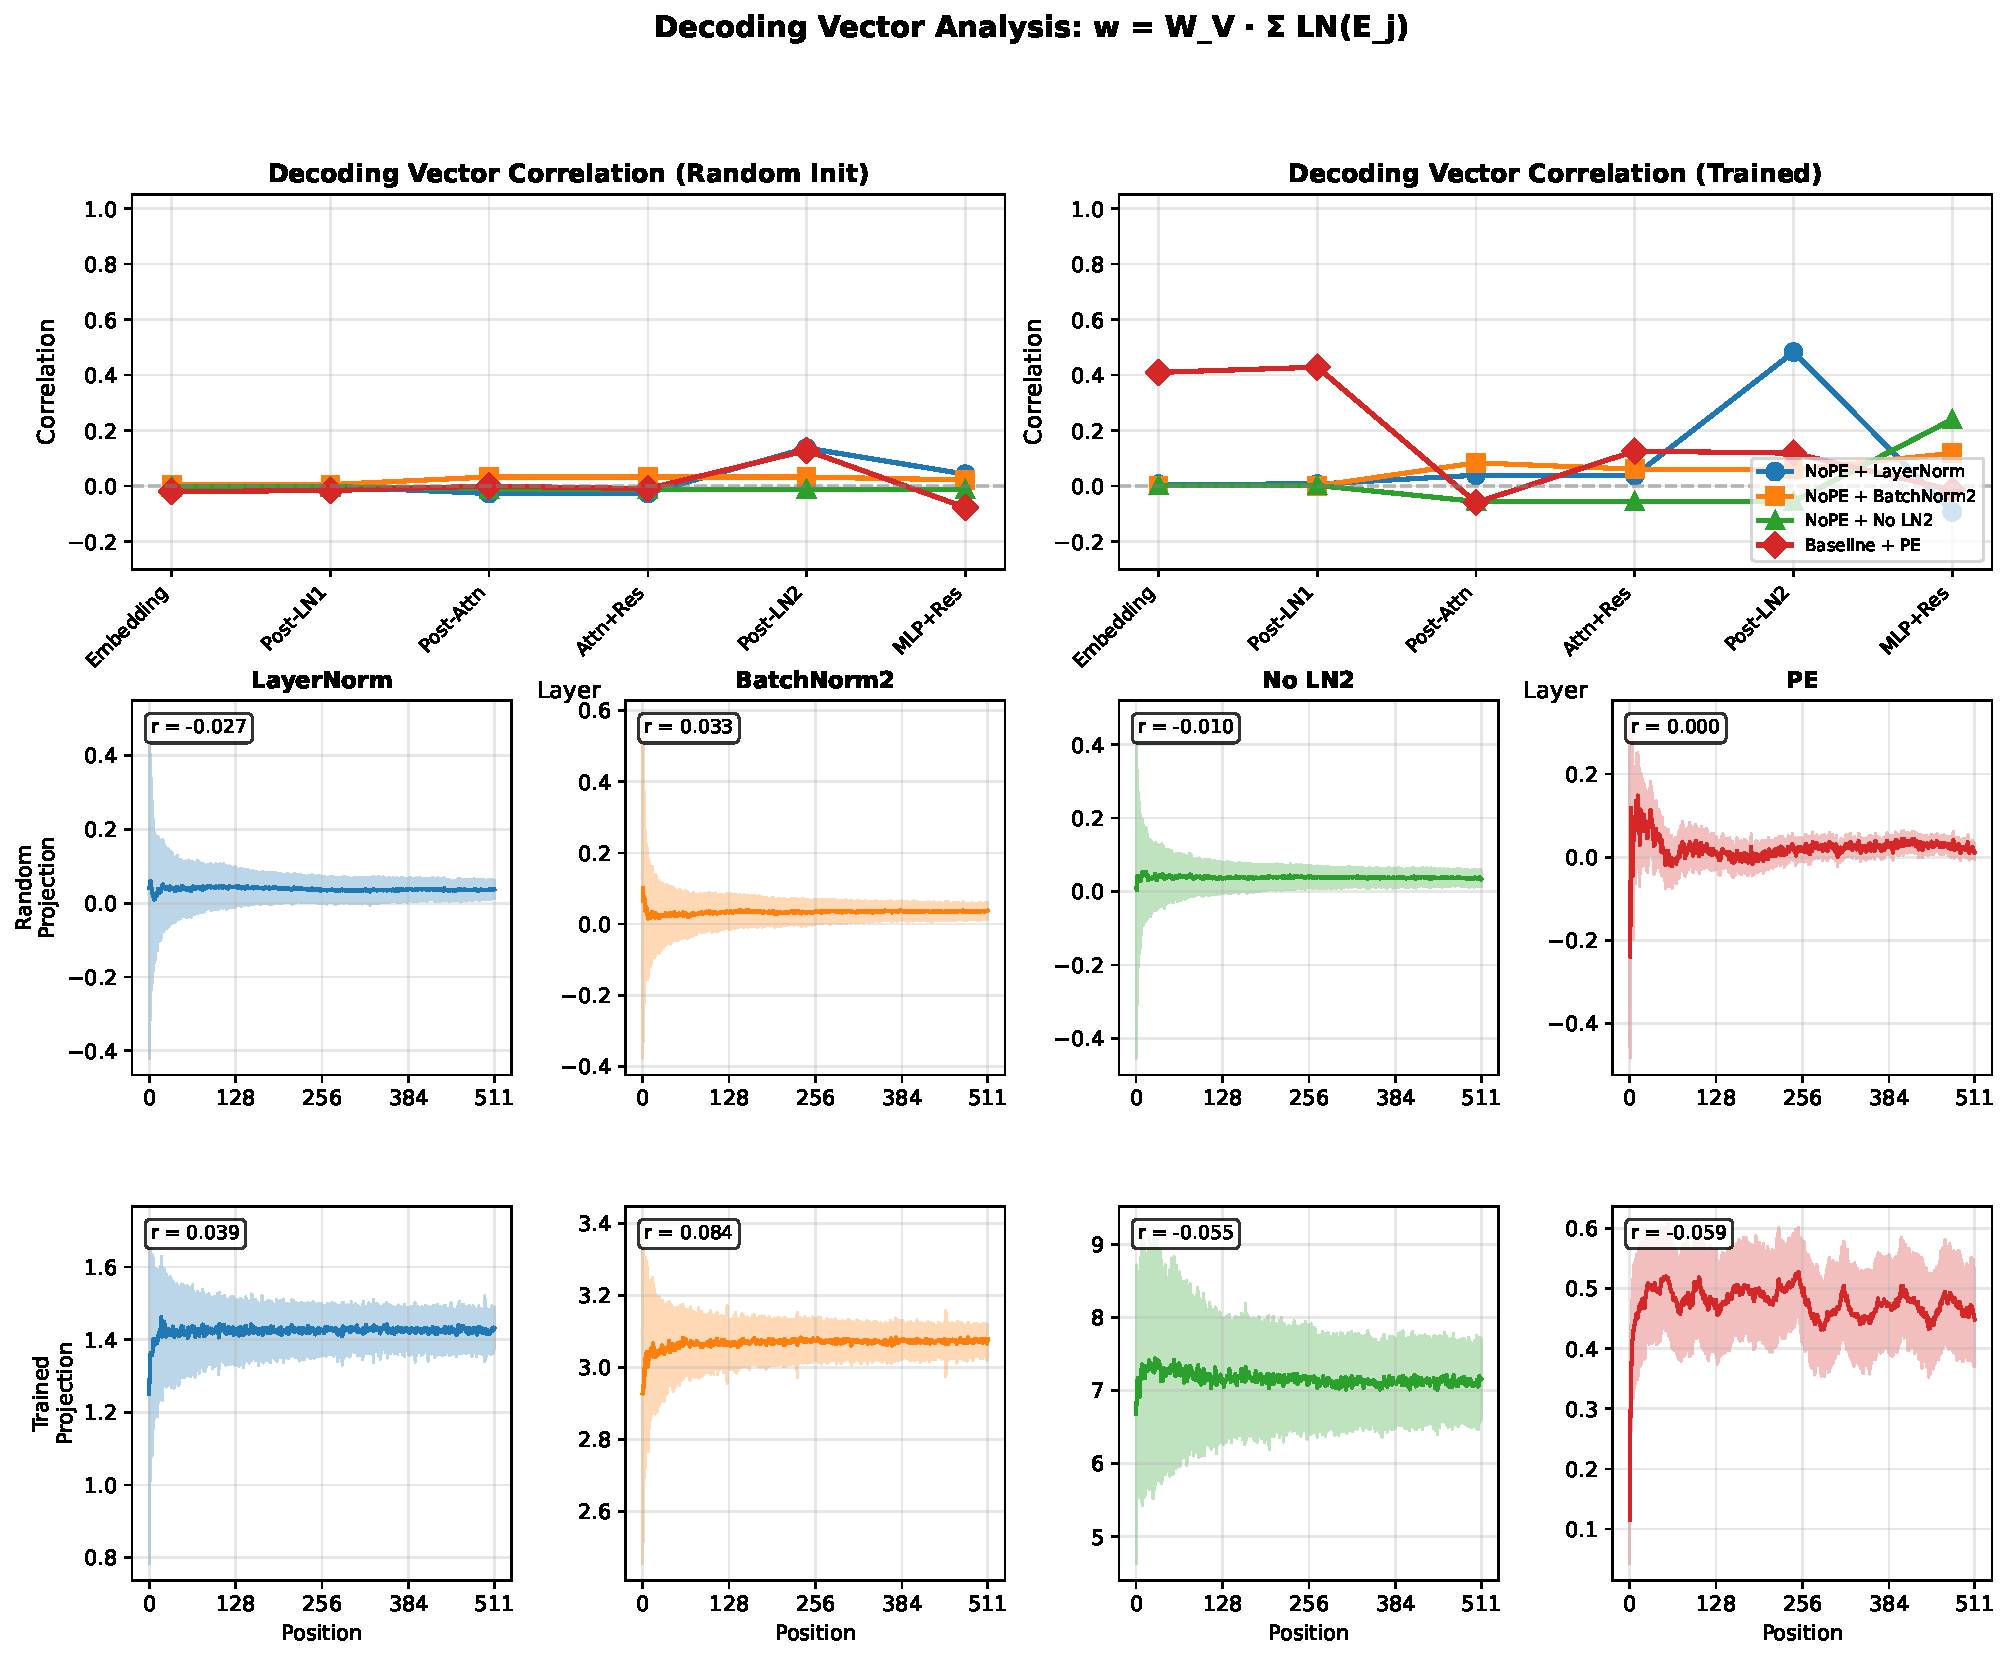
\includegraphics[width=0.9\textwidth]{plots/decoding_vector_comprehensive.pdf}
\caption{Decoding vector analysis across OWT model variants. \textbf{Top row}: Layer-wise correlation between decoding vector projection and position for random (left) and trained (right) models. NoPE + LayerNorm (blue) shows the strongest signal at post-LN2. \textbf{Bottom rows}: Mean projection vs position at post-attention for each variant, showing 100 samples. The decoding vector mechanism is most effective with LayerNorm normalization.}
\label{fig:decoding-vector-owt}
\end{figure*}

\subsection{Length Extrapolation}

We test the model's ability to generalize to longer sequences than seen during training. After training on sequences of length 64, we evaluate on sequences up to length 128. The model maintains \textbf{over 80\% accuracy} even on positions never encountered during training, demonstrating superior extrapolation capabilities compared to explicit positional embeddings which typically struggle beyond the trained context window.

\section{The LayerNorm Paradox}\label{sec:ln-paradox}

The most surprising finding in our work is what we term the LayerNorm paradox: while LayerNorm theoretically destroys all positional information by normalizing each position to zero mean and unit variance, we empirically observe that positional information not only survives but enables near-perfect position prediction exceeding 99.9\% accuracy.

\subsection{Resolution Through Population Statistics}

The paradox is resolved by recognizing that natural language exhibits position-correlated token distributions. At the individual sample level, post-LN outputs exhibit no discernible positional pattern—each position is normalized independently. However, when averaging across 500 or more samples, smooth monotonic patterns emerge as a clear function of position. This occurs because tokens that frequently appear at specific positions create consistent statistical signatures.

While LayerNorm destroys positional information within each sample, the population expectation preserves it through systematic correlations between position and token distribution. Mathematically, $\mathbb{E}_{\text{samples}}[\text{LN}(h_i)] \neq 0$ due to these position-token correlations. Figure~\ref{fig:post-ln-heatmap} visualizes these population-level patterns across 30K samples.

\begin{figure*}[htbp]
\centering
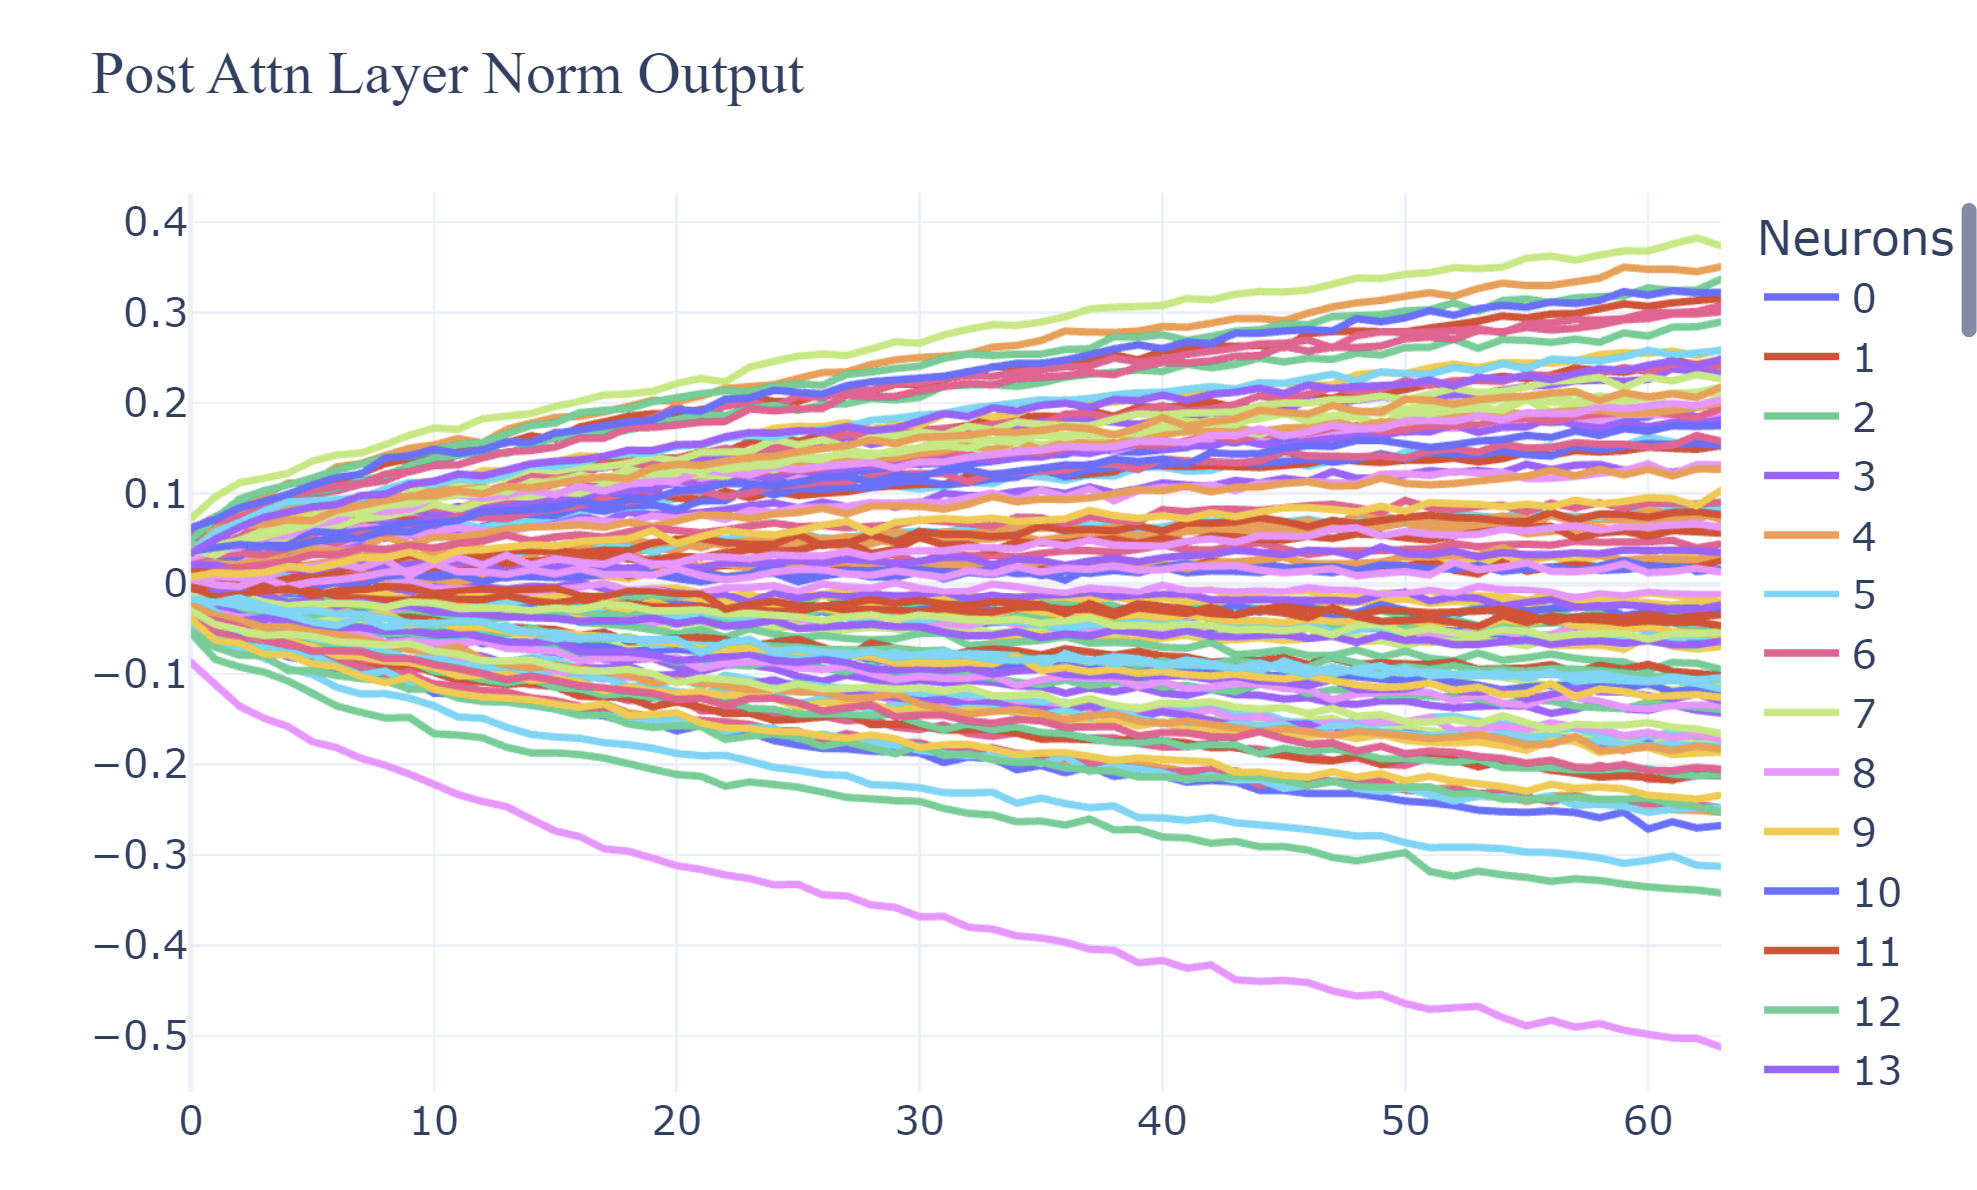
\includegraphics[width=0.9\textwidth]{post_attn_ln_output_30K_samples_64_ctx.png}
\caption{Post-LN activation patterns across 30K samples and 64 positions. Despite individual-sample normalization, clear positional structure emerges in population-level statistics. The heatmap reveals distinct patterns at different positions, with warmer colors indicating higher activation values.}
\label{fig:post-ln-heatmap}
\end{figure*}

\subsection{Sample Size Convergence}

We systematically studied how the positional pattern emerges as we increase sample size. With 10-50 samples, activations remain noisy with no discernible pattern. As sample size grows to 100-250, the pattern begins to crystallize. With 500 or more samples, we observe a stable monotonic relationship that reliably indicates position, demonstrating this is fundamentally a population-level phenomenon. Figure~\ref{fig:sample-convergence} shows this convergence.

\begin{figure*}[htbp]
\centering
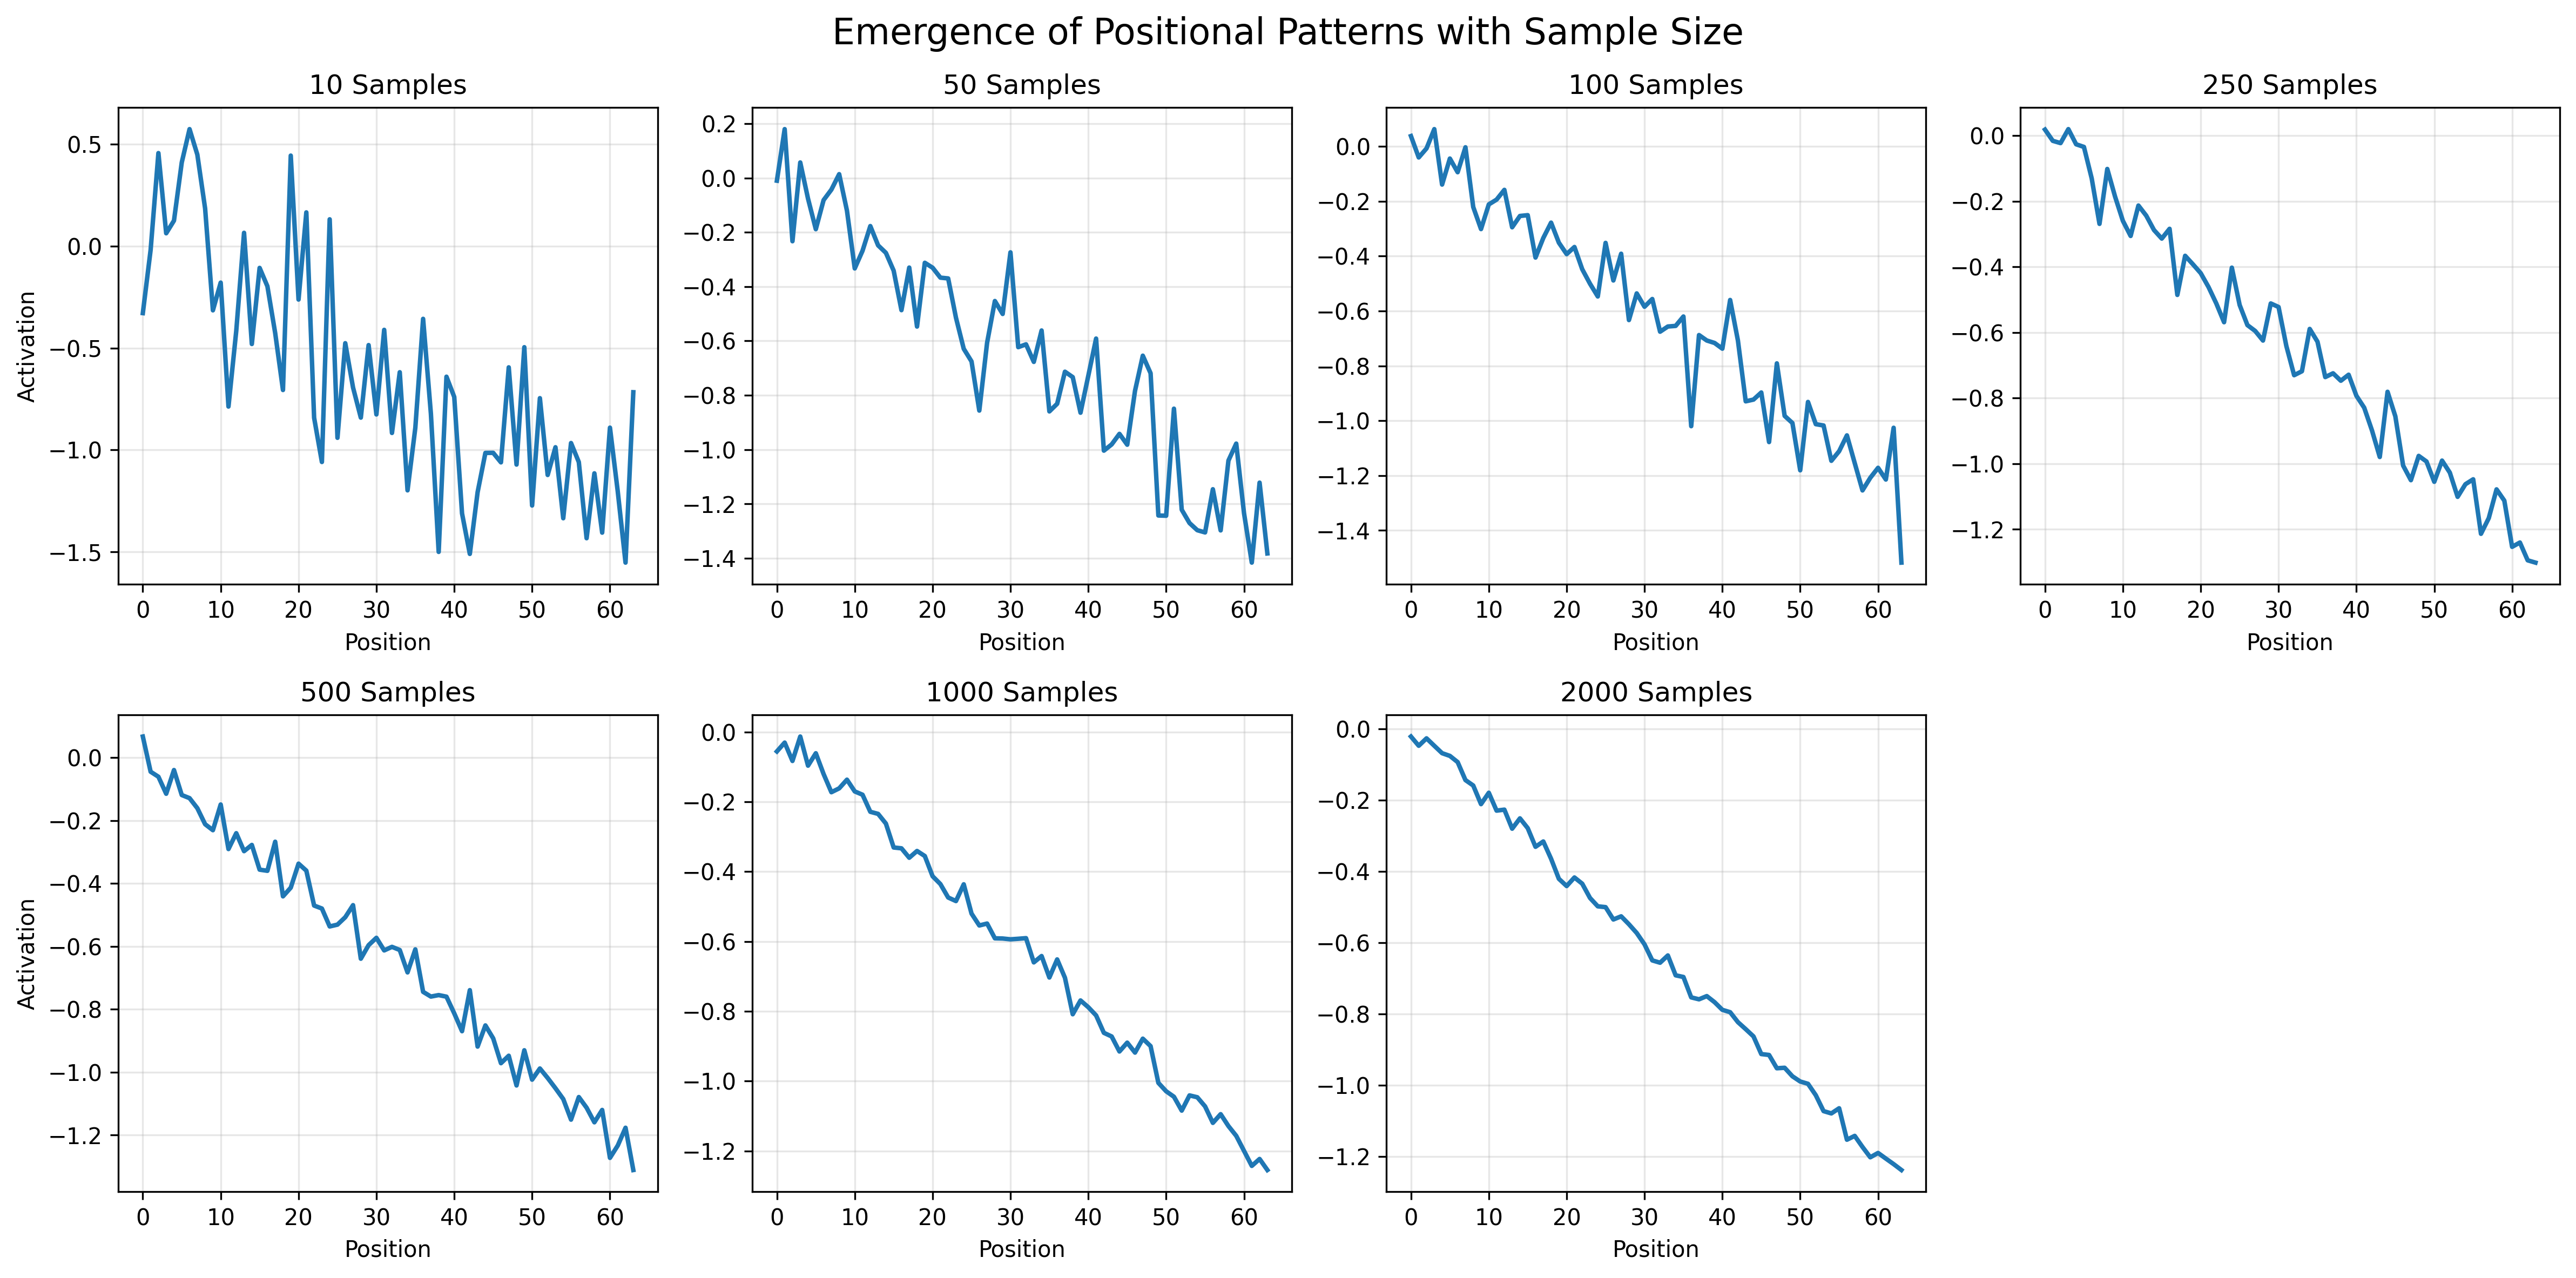
\includegraphics[width=\textwidth]{sample_convergence.png}
\caption{Emergence of positional patterns with increasing sample size from 10 to 2000 samples. The monotonic relationship becomes stable after approximately 500 samples.}
\label{fig:sample-convergence}
\end{figure*}

\subsection{Complete Circuit Characterization}

Our mechanistic analysis reveals the complete four-component circuit through layer-by-layer position probing on trained OWT models.

\subsubsection{Position Encoding at Random Initialization}

Before examining trained models, we first establish the \emph{inductive bias} for position encoding at random initialization. This reveals what positional signals exist purely from architecture, independent of learning. We train linear classifiers to predict position from activations, binning the 512 context positions into 32 groups for efficient classification (random baseline accuracy = 3.1\%).

\begin{figure*}[htbp]
\centering
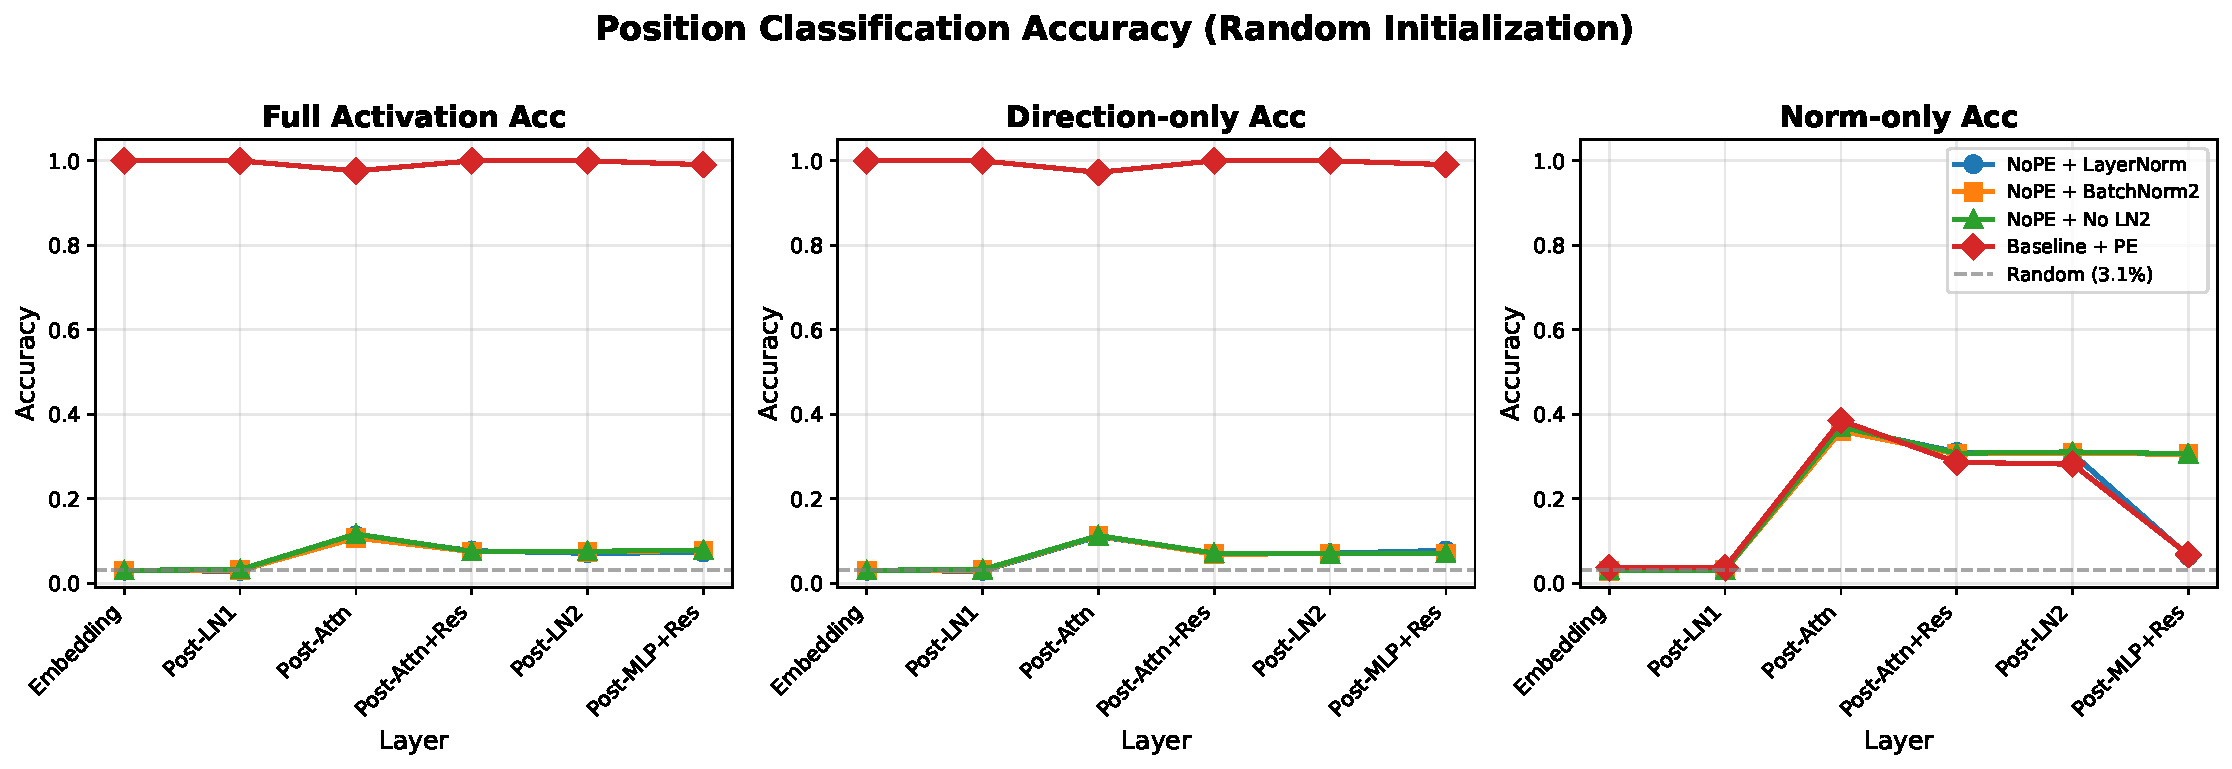
\includegraphics[width=\textwidth]{plots/owt_sample_level_accuracy_random.pdf}
\caption{Position classification accuracy at \textbf{random initialization} across layers for all four architectures. Positions are binned into 32 groups (random baseline = 3.1\%). \textbf{Key finding}: At random init, the \emph{norm} encodes position strongly (36--37\% accuracy at post-attention, 12$\times$ better than chance) while full activation and direction accuracy remain near chance (7--11\%). This confirms that causal attention averaging creates a position-dependent variance signal in the norm even before any training. The baseline with positional embeddings achieves near-perfect accuracy (99--100\%) from direction/full, as expected.}
\label{fig:sample-level-random}
\end{figure*}

Table~\ref{tab:sample-level-random} summarizes the key accuracy metrics at random initialization.

\begin{table}[htbp]
\centering
\small
\begin{tabular}{lccc}
\toprule
\textbf{Architecture} & \textbf{Post-Attn} & \textbf{Post-LN2} & \textbf{Post-MLP} \\
\midrule
\multicolumn{4}{l}{\textit{Norm Accuracy (\%)}} \\
NoPE + LN & \textbf{36.8} & 30.7 & 6.5 \\
NoPE + BN2 & 36.0 & 30.8 & 30.5 \\
NoPE + No LN2 & 37.0 & 31.1 & 30.7 \\
Baseline + PE & 38.5 & 28.2 & 6.8 \\
\midrule
\multicolumn{4}{l}{\textit{Full/Direction Accuracy (\%)}} \\
NoPE + LN & 11.3 / 11.1 & 7.1 / 7.1 & 7.3 / 7.8 \\
NoPE + BN2 & 10.7 / 11.2 & 7.5 / 7.0 & 7.8 / 7.1 \\
NoPE + No LN2 & 11.6 / 11.3 & 7.5 / 7.0 & 7.9 / 7.1 \\
Baseline + PE & 97.6 / 97.2 & 100 / 100 & 99.1 / 99.1 \\
\bottomrule
\end{tabular}
\caption{Position classification accuracy (\%) at random initialization. Random baseline = 3.1\%. \textbf{Key insight}: At init, norm accuracy (36--37\%) far exceeds full/direction accuracy (7--11\%) for NoPE models, confirming that position is initially encoded in the variance/norm created by causal attention averaging. This is the raw signal that training then transforms.}
\label{tab:sample-level-random}
\end{table}

The random initialization results reveal critical insights:

\begin{enumerate}
    \item \textbf{Norm dominates at initialization}: For all NoPE variants, norm accuracy (36--37\%) is $\sim$3--5$\times$ higher than full/direction accuracy (7--11\%). This confirms our theoretical prediction that causal attention creates a position-dependent variance signal.
    
    \item \textbf{All NoPE variants identical at init}: Before training, all normalization choices (LN, BN2, No-LN2) show identical patterns. Differences emerge only through training.
    
    \item \textbf{MLP destroys norm signal in LN variant}: NoPE+LN shows norm accuracy dropping from 30.7\% (post-LN2) to 6.5\% (post-MLP), while NoPE+BN2 and NoPE+NoLN2 preserve it ($\sim$30\%). This suggests LayerNorm enables the MLP to transform the signal differently.
\end{enumerate}

\subsubsection{Sample-Level Position Encoding in Trained Models}

After training, the picture changes dramatically.

To understand how position is encoded at the individual sample level (without population statistics), we train linear probes to predict position from activations at each layer for all four OWT architectures. Figure~\ref{fig:sample-level-probing} shows the results.

\begin{figure*}[htbp]
\centering
\includegraphics[width=\textwidth]{owt_sample_level_layerwise.pdf}
\caption{Sample-level position probing R\textsuperscript{2} across layers for all four OWT architectures. \textbf{Left}: Full activation R\textsuperscript{2}. \textbf{Center}: Direction-only R\textsuperscript{2}. \textbf{Right}: Norm-only R\textsuperscript{2}. Key observations: (1) For NoPE models, position information emerges only after attention (no signal in embeddings or post-LN1). (2) Direction dominates norm across all NoPE variants, confirming trained models encode position primarily in directional structure. (3) The baseline with positional embeddings (red) shows near-perfect position encoding from the embedding layer, with gradual decay through the network. (4) All NoPE variants achieve similar final position encoding at post-MLP ($R^2 \approx 0.3$--$0.4$) despite different normalization choices.}
\label{fig:sample-level-probing}
\end{figure*}

The results reveal several key insights about sample-level position encoding:

\begin{enumerate}
    \item \textbf{Position emerges at attention}: For all NoPE variants, there is zero positional information in embeddings or post-LN1 activations. Position first appears at post-attention, confirming that causal attention averaging is the source of the position signal.
    
    \item \textbf{Direction dominates across all layers}: In trained NoPE models, direction R\textsuperscript{2} consistently exceeds norm R\textsuperscript{2} at every layer where position is present (direction R\textsuperscript{2} $\approx 0.4$--$0.5$ vs norm R\textsuperscript{2} $\approx 0.15$--$0.25$).
    
    \item \textbf{Normalization choice affects intermediate but not final encoding}: While NoPE+LN shows a spike in full R\textsuperscript{2} at post-LN2 ($0.40$), NoPE+BN2 and NoPE+NoLN2 show different patterns. However, all converge to similar post-MLP performance ($R^2 \approx 0.31$--$0.39$).
    
    \item \textbf{Baseline+PE provides upper bound}: The standard transformer with positional embeddings achieves $R^2 > 0.98$ at early layers, demonstrating that explicit positional information is trivially decodable. This decays through the network as position mixes with content.
\end{enumerate}

Table~\ref{tab:sample-level-summary} summarizes the key metrics.

\begin{table}[htbp]
\centering
\small
\begin{tabular}{lccc}
\toprule
\textbf{Architecture} & \textbf{Post-Attn} & \textbf{Post-LN2} & \textbf{Post-MLP} \\
\midrule
\multicolumn{4}{l}{\textit{Full R\textsuperscript{2}}} \\
NoPE + LN & 0.15 & \textbf{0.40} & 0.39 \\
NoPE + BN2 & 0.15 & 0.08 & 0.31 \\
NoPE + No LN2 & 0.12 & 0.12 & 0.39 \\
Baseline + PE & 0.98 & 0.65 & 0.49 \\
\midrule
\multicolumn{4}{l}{\textit{Direction R\textsuperscript{2}}} \\
NoPE + LN & 0.46 & 0.38 & 0.42 \\
NoPE + BN2 & 0.34 & 0.44 & 0.42 \\
NoPE + No LN2 & \textbf{0.50} & \textbf{0.53} & \textbf{0.50} \\
Baseline + PE & 0.97 & 0.65 & 0.49 \\
\bottomrule
\end{tabular}
\caption{Sample-level position probing R\textsuperscript{2} at key layers. NoPE+NoLN2 shows the highest direction R\textsuperscript{2}, suggesting that skipping normalization preserves more directional position information. NoPE+LN shows a unique spike in full R\textsuperscript{2} at post-LN2, indicating LayerNorm creates a more linear position signal.}
\label{tab:sample-level-summary}
\end{table}

\subsection{MLP Probe Analysis: Non-linear Decodability}

To further characterize the nature of positional encoding, we train \textbf{MLP probes} alongside linear probes on the same activations. MLP probes have greater expressive capacity and can capture non-linear relationships. Since MLPs cannot encode position by themselves (they lack positional inductive bias), if an MLP probe succeeds where a linear probe fails, this indicates that positional information is present but encoded non-linearly.

We compare MLP and linear probes across all four OWT architectures (NoPE+LN, NoPE+BN2, NoPE+NoLN2, Baseline+PE) at both random initialization and after training. Figure~\ref{fig:mlp-probes-fig1} shows the R\textsuperscript{2} scores for both probe types at each activation point, while Figure~\ref{fig:mlp-probes-fig2} shows the MLP advantage (MLP R\textsuperscript{2} $-$ Linear R\textsuperscript{2}).

\begin{figure*}[htbp]
\centering
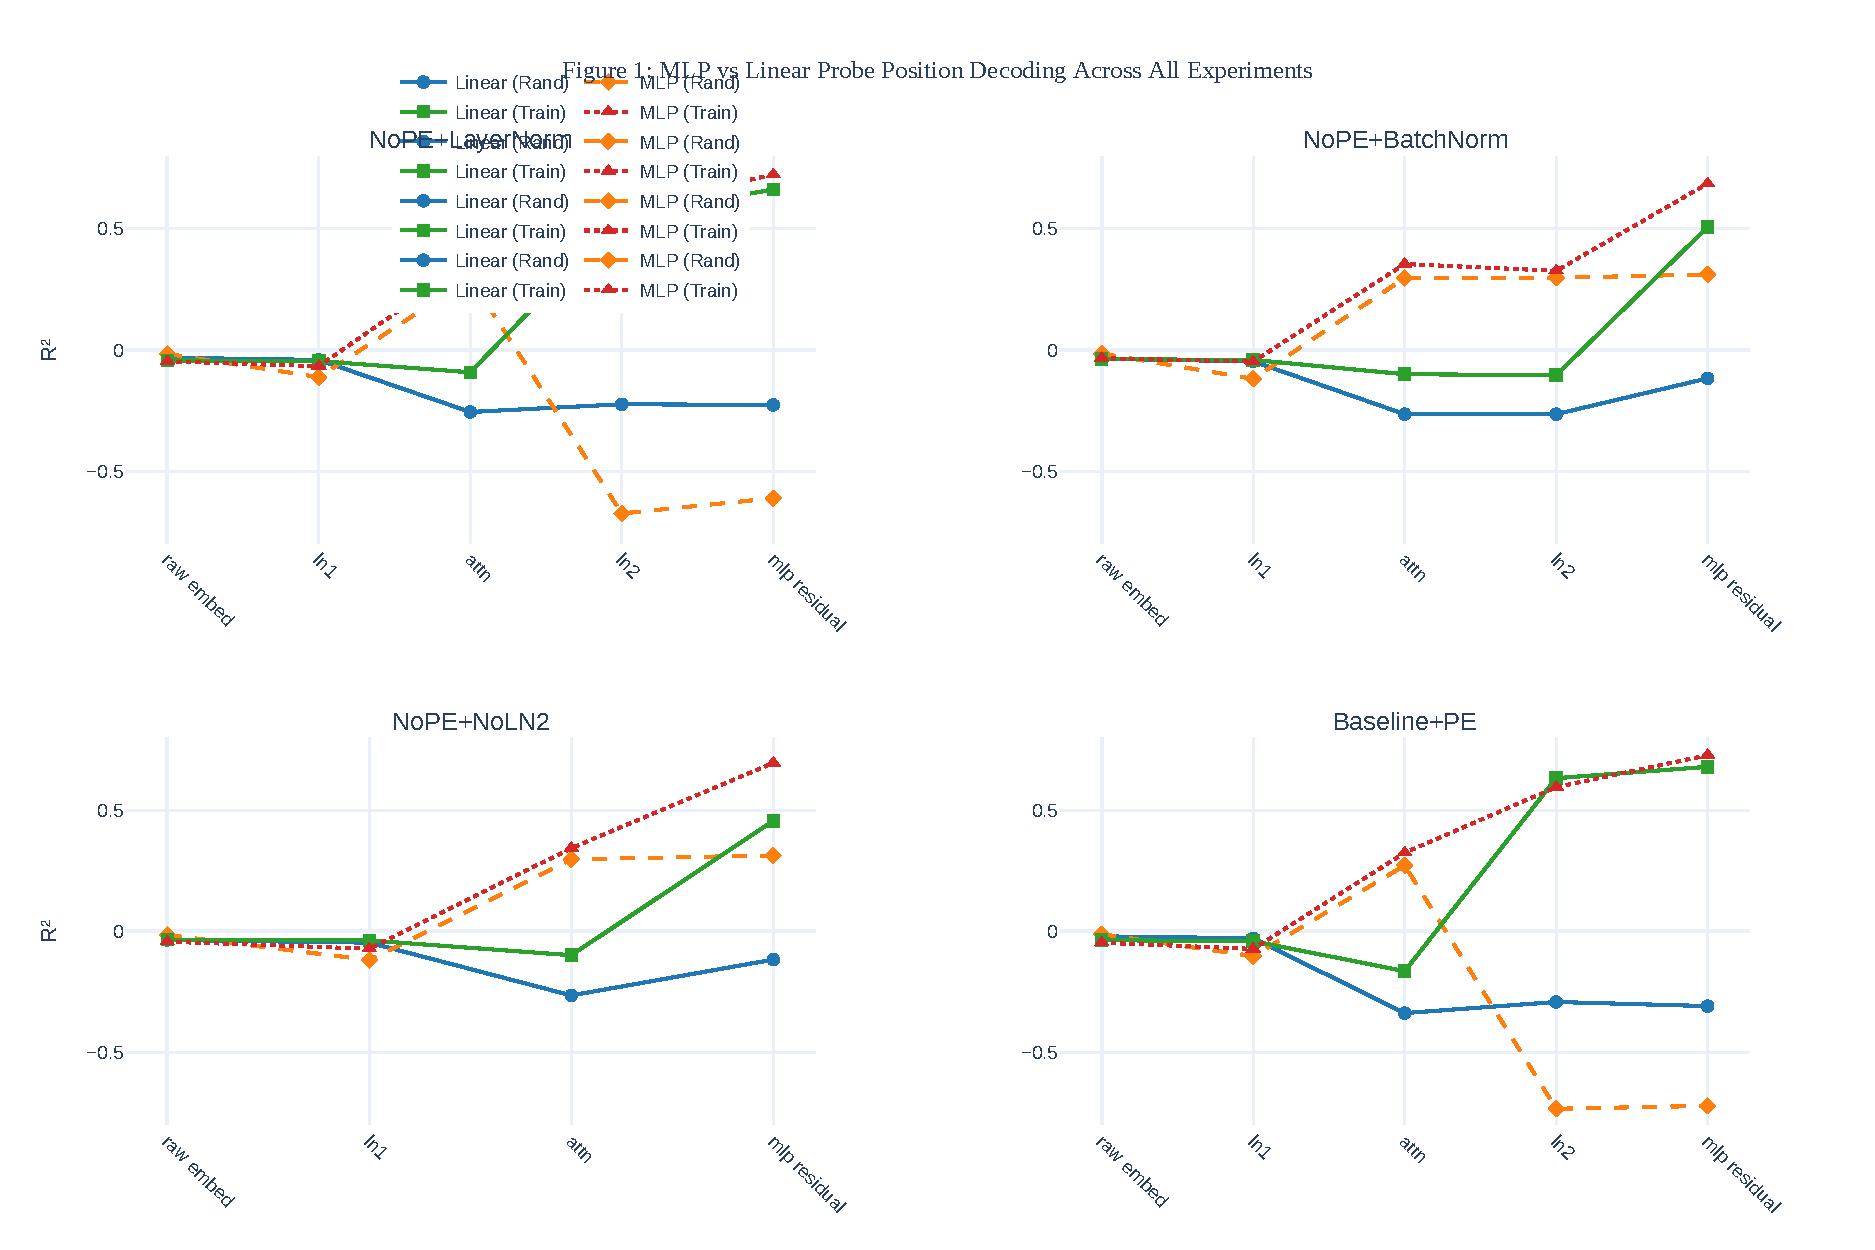
\includegraphics[width=\textwidth]{mlp_probes_fig1.pdf}
\caption{MLP vs Linear probe position decoding R\textsuperscript{2} across all four OWT architectures. Solid lines: Linear probes. Dashed lines: MLP probes. Blue/Green: Random initialization. Orange/Red: Trained models. Key finding: MLP probes significantly outperform linear probes at post-attention layers in random models, indicating that position is initially encoded in non-linear form before being linearized by LayerNorm.}
\label{fig:mlp-probes-fig1}
\end{figure*}

\begin{figure*}[htbp]
\centering
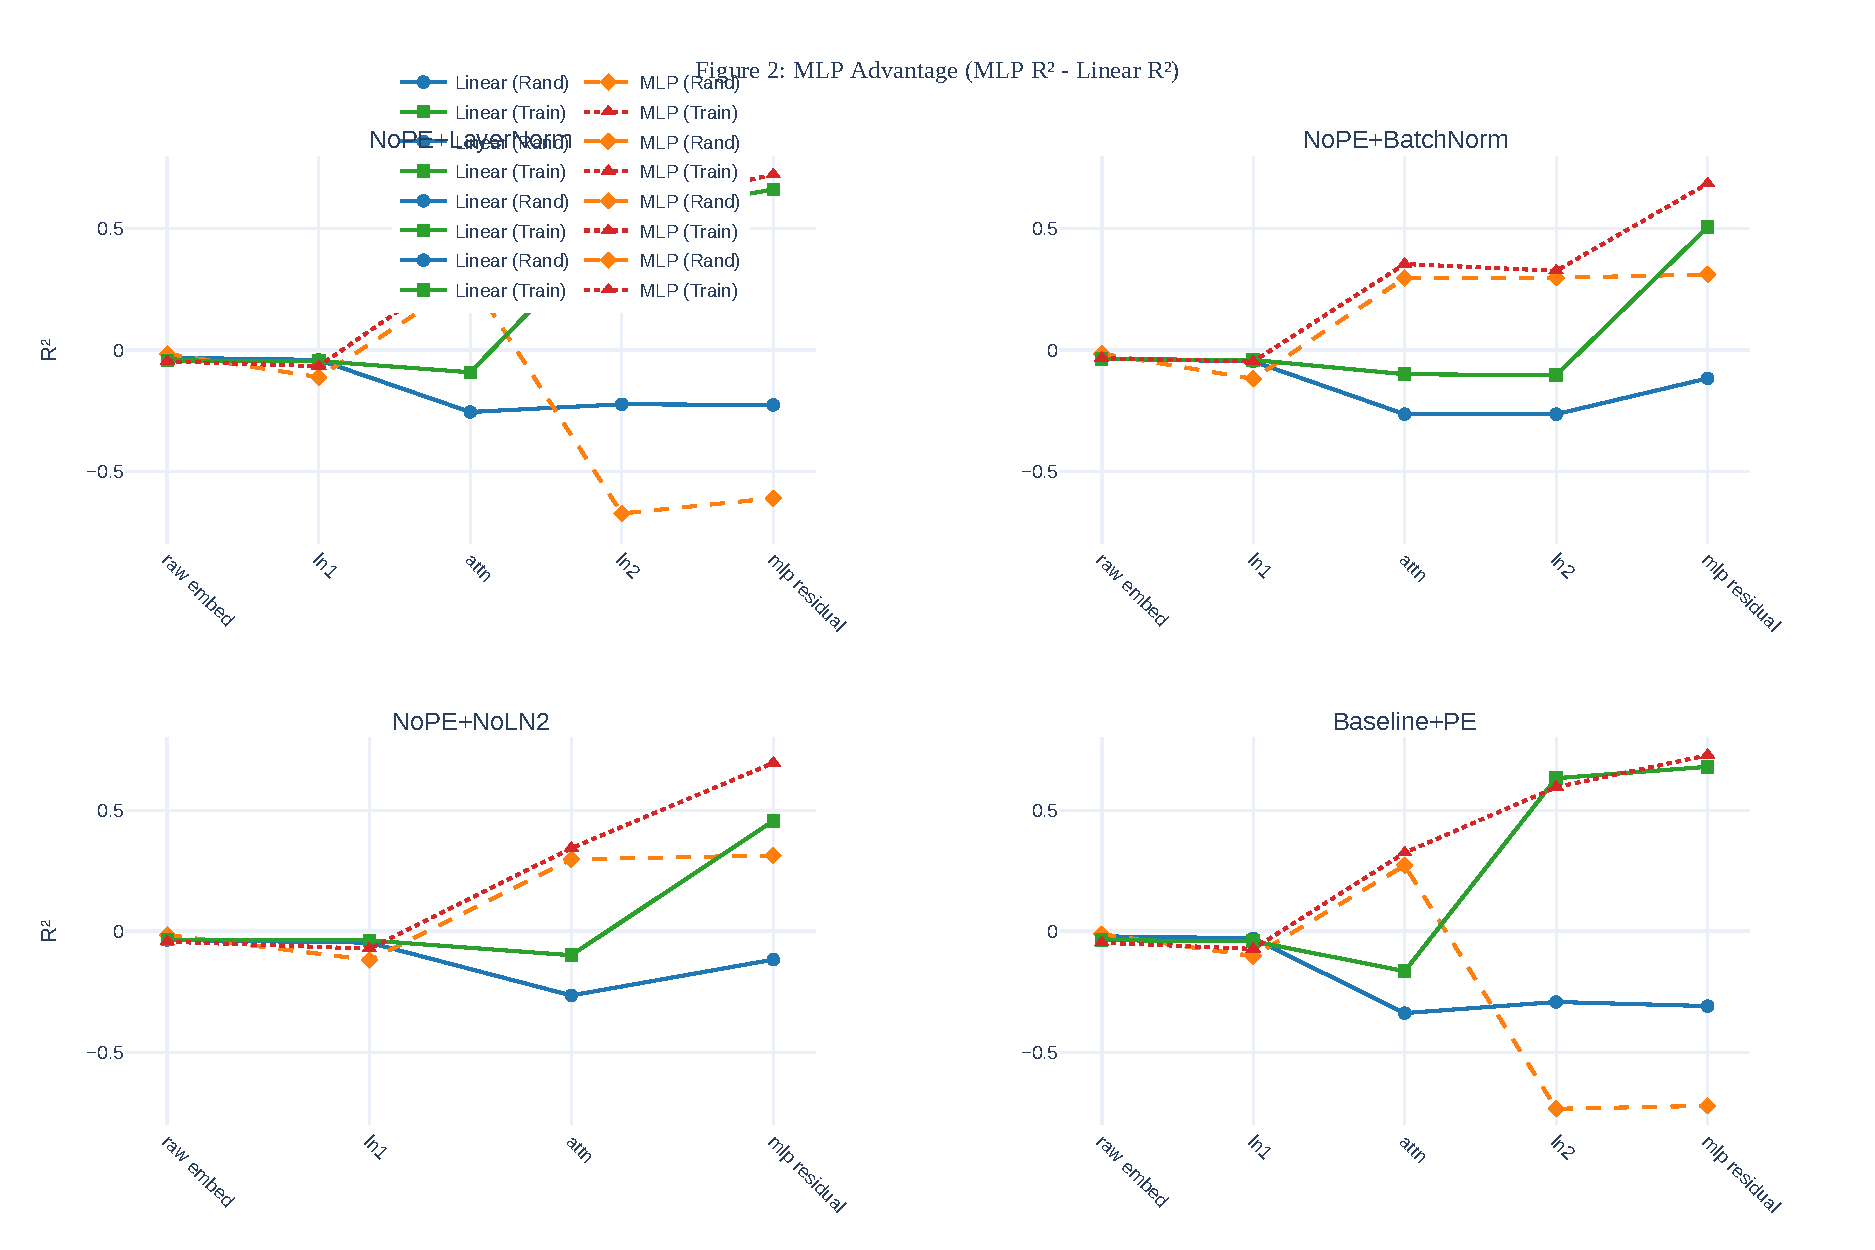
\includegraphics[width=\textwidth]{mlp_probes_fig2.pdf}
\caption{MLP advantage (MLP R\textsuperscript{2} $-$ Linear R\textsuperscript{2}) across all experiments. Positive values (green) indicate where MLP outperforms linear probes. Key findings: (1) In random models, MLP probes show strong advantage at post-attention ($+0.3$ to $+0.5$ R\textsuperscript{2}), confirming non-linear position encoding before LayerNorm. (2) In trained models, the advantage diminishes at post-LN2 layers where LayerNorm has linearized the signal. (3) The Baseline+PE model shows minimal MLP advantage, consistent with explicit positional embeddings providing linearly decodable position information.}
\label{fig:mlp-probes-fig2}
\end{figure*}

The MLP probe analysis reveals three key insights:

\begin{enumerate}
    \item \textbf{Non-linear encoding before LayerNorm}: At random initialization, MLP probes substantially outperform linear probes at post-attention layers (MLP advantage $+0.3$ to $+0.5$ R\textsuperscript{2}). This confirms our theoretical analysis that position is initially encoded in complex, non-linear directional structure that requires non-linear decoding.
    
    \item \textbf{LayerNorm linearizes the signal}: After LayerNorm (post-LN2), the MLP advantage largely disappears, with linear and MLP probes achieving similar R\textsuperscript{2}. This provides direct empirical evidence that LayerNorm transforms the non-linear position encoding into a linearly decodable form (primarily through the norm-based mechanism).
    
    \item \textbf{Training preserves some non-linearity}: In trained models, the MLP advantage re-emerges at post-MLP layers, suggesting that the MLP transforms the linearly-encoded position signal back into a more complex form that requires non-linear probing. This may reflect learned position-dependent transformations.
    
    \item \textbf{NoPE variants behave similarly}: All three NoPE variants (LN, BN2, NoLN2) show the same qualitative pattern: strong MLP advantage at post-attention, minimal advantage at post-LN2, and partial recovery at post-MLP. The normalization choice affects the magnitude but not the qualitative nature of these effects.
\end{enumerate}

These results provide strong support for our four-component circuit model: (1) causal attention creates non-linear position encoding in attention outputs, (2) LayerNorm linearizes this into a norm-based signal, (3) the MLP transforms the signal, and (4) the final representation combines both linearly and non-linearly decodable position information.

\subsection{Token Distribution Manipulation}

We validate the necessity of position-token correlations through controlled experiments. When token distributions are perfectly uniform across positions, the mechanism fails completely with correlation near zero. With position-correlated distributions matching natural language patterns, the model achieves strong performance with correlation exceeding 0.6. Even with anti-correlated distributions where position-token relationships are inverted, the model produces an inverted but still functional pattern, demonstrating sensitivity to any systematic position-token relationship.

\section{Discussion}

Our discovery of implicit positional encoding has several important implications for understanding transformer architectures. First, the fact that positional information can be encoded without explicit embeddings suggests that transformer capabilities are more distributed across architectural components than previously thought. The interaction between initialization, attention patterns, normalization, and data statistics creates emergent computational abilities.

Second, the mechanism highlights the critical importance of data statistics in enabling architectural capabilities. The circuit relies on position-correlated token distributions found naturally in language, suggesting that successful model design requires understanding the statistical structure of training data.

Third, understanding this implicit mechanism opens avenues for designing more efficient transformers. The variance-based positional signal may extrapolate better to longer sequences than learned positional embeddings, which are constrained to the training context length.

\section{Conclusion}

Prior work established that causal transformers can encode position implicitly \citep{haviv2022transformer, chi-etal-2023-latent}; we contribute the first complete mechanistic circuit explaining \textit{how} this occurs. We have identified a four-component circuit enabling causal transformers to encode absolute positional information without explicit positional embeddings. The circuit consists of token embedding diversity providing rich representations, near-uniform causal attention creating position-dependent variance signals, LayerNorm that paradoxically preserves positional information through population-level statistics, and MLPs that decode position using a single decoding vector $w = W_V \cdot \sum_j \text{LN}(E_j)$. The decoding achieves Pearson correlation $r = 0.999$ between decoded and true positions.

Our key discovery---the LayerNorm paradox---reveals that positional information survives normalization through token repetition patterns in natural language. While LayerNorm eliminates positional signals from individual samples, averaging across many samples exposes monotonic positional patterns because certain tokens appear more frequently at specific positions.

Crucially, our causal intervention experiments disentangle the contributions of the two decoding mechanisms. We find that geometric decoding via individual sample features is \textbf{sufficient} for position prediction---probes trained on mean-subtracted activations achieve nearly identical accuracy to baseline probes (0.3\% relative drop). However, trained probes will \textbf{utilize} population statistics when available, as evidenced by the 53\% accuracy drop when population means are removed at test time. This reveals that while the circuit provides multiple pathways for position encoding, the geometric mechanism based on embedding orthogonality is the primary driver. The circuit achieves over 99.9\% accuracy across multiple normalization schemes while providing better length extrapolation compared to explicit positional embeddings.

\section*{Limitations}

Our work has several limitations. \textbf{Most critically, our analysis reveals that the norm-based position encoding mechanism is largely an initialization phenomenon}---training dramatically reduces the norm-position correlation from $r=-0.97$ to $r=+0.15$ (Section~\ref{sec:random-vs-trained}). While trained NoPE models still function, they appear to use different mechanisms than the initialization-time circuit we characterize. This suggests our findings are most relevant for understanding inductive biases rather than learned representations.

While our intervention experiments demonstrate that the geometric decoding mechanism can function on individual samples without population statistics, the population-level patterns still provide additional signal that trained models utilize when available. The circuit requires sufficient token embedding diversity, limiting applicability to domains with very small vocabularies. We observe initialization sensitivity, as the mechanism requires careful initialization within specific variance ranges (Xavier-scale) for optimal performance. The absolute accuracy of isolated probes (3-5\%) is substantially lower than the full trained model (99.97\%), indicating that the complete circuit involves interactions beyond what our intervention experiments capture. Finally, our analysis focuses on single-layer models; multi-layer interactions may introduce additional complexities not captured here.

\section*{Future Work}

The discovery of implicit positional encoding opens several research directions including multi-layer circuit analysis to understand how the mechanism evolves across deep transformers, cross-modal generalization to examine whether similar mechanisms emerge in vision transformers, and developing theoretical foundations for when and how normalization layers preserve information through population statistics.

\bibliographystyle{acl_natbib}
\bibliography{custom}

\appendix

\section{LayerNorm Norm Statistics}\label{sec:ln-norm-derivation}

We model each pre-LN activation $h_i \in \mathbb{R}^d$ at position $i$ as approximately Gaussian with zero mean and covariance $\sigma_i^2 I$, where $\sigma_i^2 \propto 1/(i{+}1)$ comes from averaging $i{+}1$ value vectors under near-uniform attention. Let $d$ be large. PyTorch LayerNorm uses the biased variance estimator
\[
\hat\sigma_i^2 = \frac{1}{d} \sum_{k=1}^d (h_{i,k} - \bar{h}_i)^2,
\]
so for Gaussian inputs $\mathbb{E}[\hat\sigma_i^2] = \tfrac{d-1}{d} \sigma_i^2$ and the normalized vector is
\[
\text{LN}(h_i) = \gamma \cdot \frac{h_i - \bar{h}_i}{\hat\sigma_i} + \beta.
\]
A first-order delta-method expansion around $\hat\sigma_i^2 \approx \sigma_i^2$ gives
\[
\mathbb{E}\big[\|\text{LN}(h_i)\|\big] \approx \|\gamma\| \sqrt{d} \Big(1 + \frac{\kappa_i - 3}{8d} + \delta_i\Big),
\]
where $\kappa_i$ is the (position-dependent) kurtosis of $h_i$ (approaching 3 as $i$ grows) and $\delta_i = \mathcal{O}(1/d)$ captures the bias from $d$ vs. $d{-}1$. Because $\kappa_i$ drifts smoothly with $\sigma_i^2$, the expected norm inherits a tiny but monotone dependence on position, producing the residual trend seen in Fig.~\ref{fig:norm-over-positions}. Empirically, this residual is small in magnitude (e.g., norms in $[27.54, 27.71]$ for the random Shakespeare model) but sufficiently systematic to yield high norm-only $R^2$.

\section{NoPE Language Model Training Details}\label{app:nope-training}

This appendix provides complete details for reproducing the NoPE language model experiments described in Section 4.6.

\subsection{Architecture}

We use a GPT-style decoder-only transformer with the following configuration:

\begin{table}[htbp]
\centering
\small
\begin{tabular}{ll}
\toprule
\textbf{Parameter} & \textbf{Value} \\
\midrule
Number of layers & 1 \\
Number of attention heads & 12 \\
Embedding dimension & 768 \\
MLP hidden dimension & 3072 (4$\times$) \\
Context length & 256 \\
Vocabulary size & 50,304 (GPT-2 BPE) \\
Dropout & 0.0 \\
Bias & False \\
Positional embedding & \textbf{Disabled} \\
\bottomrule
\end{tabular}
\caption{NoPE model architecture parameters.}
\label{tab:nope-arch}
\end{table}

The key modification is disabling positional embeddings entirely---no sinusoidal, learned, rotary, or any other positional encoding is used. We train two variants differing only in normalization: LayerNorm (centering + scaling) and RMSNorm (scaling only).

\subsection{Initialization}

We use Xavier (Glorot) normal initialization for all weight matrices, particularly the attention Q, K, V projections. This ensures near-uniform attention at initialization, as discussed in Section 3.2. Specifically:
\begin{equation}
W \sim \mathcal{N}\left(0, \frac{2}{n_{\text{in}} + n_{\text{out}}}\right)
\end{equation}

\subsection{Training Configuration}

\begin{table}[htbp]
\centering
\small
\begin{tabular}{ll}
\toprule
\textbf{Parameter} & \textbf{Value} \\
\midrule
Dataset & Shakespeare (BPE tokenized) \\
Dataset size & $\sim$302K tokens \\
Batch size & 32 \\
Gradient accumulation steps & 4 \\
Effective batch size & 128 \\
Learning rate & $10^{-3}$ \\
Learning rate schedule & Cosine decay \\
Warmup iterations & 200 \\
Total iterations & 5000 \\
Optimizer & AdamW \\
$\beta_1$, $\beta_2$ & 0.9, 0.95 \\
Weight decay & 0.1 \\
Gradient clipping & 1.0 \\
Random seed & 42 \\
\bottomrule
\end{tabular}
\caption{NoPE model training hyperparameters.}
\label{tab:nope-training}
\end{table}

\subsection{Results Summary}

\begin{table}[htbp]
\centering
\small
\begin{tabular}{lcc}
\toprule
\textbf{Model} & \textbf{Val Loss} & \textbf{Perplexity} \\
\midrule
NoPE + LayerNorm & 5.743 & 311.9 \\
NoPE + RMSNorm & 5.792 & 327.6 \\
\bottomrule
\end{tabular}
\caption{Final validation metrics for trained NoPE models.}
\label{tab:nope-results}
\end{table}

Both models converge to similar perplexities, indicating that the language modeling objective does not require positional information to achieve reasonable performance on this dataset. The slightly higher perplexity of the RMSNorm variant may reflect the lack of mean-centering, though both perform adequately for a single-layer model.

\subsection{Hypothesis Validation Details}

\paragraph{H1: Attention Uniformity.} We computed the variance of attention weights at each position and compared to the theoretical $1/(i+1)$ decay. All 12 heads in both models showed Pearson $r > 0.99$ correlation with the theoretical curve, confirming that near-uniform attention persists through training.

\paragraph{H2: Population Statistics.} Linear probes trained on population means (averaged across 5000 samples) achieve $r = 1.0$ between probe predictions and true positions, confirming that position-correlated token distributions create exploitable patterns in the mean activations through the LayerNorm paradox mechanism.

\section{Experimental Conditions for Figures and Tables}\label{app:experimental-conditions}

This appendix documents the exact experimental conditions used to generate each figure and table in the paper. Different experiments use different model configurations and data sources; this section provides full provenance for reproducibility.

\subsection{Model Configurations}

We use three distinct model configurations across experiments:

\begin{table}[htbp]
\centering
\small
\begin{tabular}{lccc}
\toprule
\textbf{Config} & \textbf{Synthetic-Small} & \textbf{Synthetic-Large} & \textbf{Trained} \\
\midrule
Model state & Random init & Random init & Trained 5K steps \\
n\_embd & 256 & 768 & 768 \\
n\_head & 4 & 12 & 12 \\
n\_ctx & 64 & 64 & 256 \\
vocab\_size & 1,000 & 50,257 & 50,304 \\
Input tokens & Uniform random & Uniform random & Shakespeare \\
\bottomrule
\end{tabular}
\caption{Model configurations used across experiments.}
\label{tab:model-configs}
\end{table}

\subsection{Figure and Table Provenance}

\begin{table}[htbp]
\centering
\small
\begin{tabular}{lll}
\toprule
\textbf{Figure/Table} & \textbf{Config} & \textbf{Source Script} \\
\midrule
\multicolumn{3}{l}{\textit{Main paper figures}} \\
Fig.~\ref{fig:single-sample-pred} & Synthetic-Large & \texttt{layernorm\_paradox\_investigation.py} \\
Fig.~\ref{fig:attention-patterns} & Synthetic-Large & \texttt{attention\_std\_phases.py} \\
Fig.~\ref{fig:variance-decay} & Synthetic-Large & \texttt{generate\_all\_paper\_figures.py} \\
Fig.~\ref{fig:ln-linearization} & Synthetic-Small & \texttt{direction\_norm\_independence.py} \\
Fig.~\ref{fig:layernorm-paradox} & Synthetic-Large & \texttt{layernorm\_paradox\_investigation.py} \\
Fig.~\ref{fig:mlp-contributions} & Synthetic (d=1024) & \texttt{mlp\_decoding\_peaks.py} \\
Fig.~\ref{fig:mlp-decoding} & Synthetic (d=1024) & \texttt{mlp\_decoding\_peaks.py} \\
Fig.~\ref{fig:vocab-scaling} & Synthetic (varied) & \texttt{vocabulary\_scaling\_linear.py} \\
Fig.~\ref{fig:critical-neurons} & Synthetic-Large & \texttt{layernorm\_paradox\_investigation.py} \\
Fig.~\ref{fig:neuron-avg-activations} & Synthetic-Large & \texttt{layernorm\_paradox\_investigation.py} \\
\midrule
\multicolumn{3}{l}{\textit{Direction vs norm analysis}} \\
Tab.~\ref{tab:direction-norm} & Synthetic-Small & \texttt{direction\_norm\_independence.py} \\
Fig.~\ref{fig:norm-over-positions} & Synthetic-Large + Trained & \texttt{visualize\_norm\_over\_positions.py} \\
\midrule
\multicolumn{3}{l}{\textit{Random vs trained comparison}} \\
Tab.~\ref{tab:random-vs-trained} & Trained + Random & \texttt{trained\_model\_analysis.py} \\
Fig.~\ref{fig:trained-vs-random} & Trained + Random & \texttt{visualize\_norm\_over\_positions.py} \\
\midrule
\multicolumn{3}{l}{\textit{Appendix figures}} \\
Fig.~\ref{fig:post-ln-heatmap} & Synthetic-Large & \texttt{layernorm\_paradox\_investigation.py} \\
Fig.~\ref{fig:sample-convergence} & Synthetic-Large & \texttt{sample\_convergence\_analysis.py} \\
\bottomrule
\end{tabular}
\caption{Experimental conditions for each figure and table.}
\label{tab:figure-provenance}
\end{table}

\subsection{Key Values by Experiment}

\paragraph{Table~\ref{tab:direction-norm} (Direction vs Norm R\textsuperscript{2}).} 
Values from \texttt{direction\_norm\_independence\_results.json} using \textbf{Synthetic-Small} config:
\begin{itemize}
    \item post\_attn: Full $R^2=0.04$, Norm $R^2=0.56$, Direction $R^2=0.39$
    \item post\_ln2: Full $R^2=0.19$, Norm $R^2=0.88$, Direction $R^2=0.19$
    \item post\_mlp\_residual: Full $R^2=0.22$, Norm $R^2=0.39$, Direction $R^2=0.35$
\end{itemize}

\paragraph{Table~\ref{tab:random-vs-trained} (Random vs Trained).}
Values from \texttt{trained\_model\_results.json} using \textbf{Trained} config on Shakespeare:
\begin{itemize}
    \item Random Init: norm-position $r=-0.97$, norm $R^2=0.94$, direction $R^2=0.23$
    \item Trained LN: norm-position $r=+0.15$, norm $R^2=0.02$, direction $R^2=0.18$
\end{itemize}

\paragraph{Figure~\ref{fig:norm-over-positions} (Norm Over Positions).}
Generated by \texttt{visualize\_norm\_over\_positions.py} using \textbf{Synthetic-Large} (random) and \textbf{Trained} (LayerNorm) configs with uniform random tokens (n\_ctx=64). The correlations shown ($r=-0.998$ random, $r=+0.86$ trained) are computed within the script on this specific setup and differ from Table~\ref{tab:random-vs-trained} values due to:
\begin{enumerate}
    \item Different context length (64 vs 256)
    \item Different input tokens (uniform random vs Shakespeare)
    \item Different sample sizes
\end{enumerate}

\paragraph{Tables~\ref{tab:owt-dir-norm}, \ref{tab:owt-linearization}, \ref{tab:owt-population} (OWT Experiments).}
Generated by \texttt{owt\_comprehensive\_analysis.py}, \texttt{owt\_layernorm\_linearization.py}, and \texttt{owt\_batchnorm\_population.py} using models trained on OpenWebText for 50K iterations. All models use 1 layer, 12 heads, 768 embedding dimensions, and 512 context length. Results stored in \texttt{results/owt\_comprehensive/}.

\subsection{Reconciling Different R\textsuperscript{2} Values}

The paper reports several sets of R\textsuperscript{2} values that may appear inconsistent but arise from different experimental conditions:

\begin{enumerate}
    \item \textbf{$R^2_{\text{norm}}=0.88$ (post-LN)} from Table~\ref{tab:direction-norm}: Synthetic-Small config, n\_embd=256, uniform tokens
    \item \textbf{$R^2_{\text{norm}}=0.94$ (post-LN)} from Table~\ref{tab:random-vs-trained}: Random init with n\_embd=768 on Shakespeare
    \item \textbf{$r=-0.998$} in Fig.~\ref{fig:norm-over-positions}: Random n\_embd=768, uniform tokens, n\_ctx=64
\end{enumerate}

These differences reflect how the positional encoding mechanism scales with model size and responds to different input distributions. The core finding---that LayerNorm linearizes position encoding from direction into norm---is consistent across all conditions.

\end{document}